\documentclass[twoside]{book}

% Packages required by doxygen
\usepackage{fixltx2e}
\usepackage{calc}
\usepackage{doxygen}
\usepackage{graphicx}
\usepackage[utf8]{inputenc}
\usepackage{makeidx}
\usepackage{multicol}
\usepackage{multirow}
\PassOptionsToPackage{warn}{textcomp}
\usepackage{textcomp}
\usepackage[nointegrals]{wasysym}
\usepackage[table]{xcolor}

% Font selection
\usepackage[T1]{fontenc}
\usepackage{mathptmx}
\usepackage[scaled=.90]{helvet}
\usepackage{courier}
\usepackage{amssymb}
\usepackage{sectsty}
\renewcommand{\familydefault}{\sfdefault}
\allsectionsfont{%
  \fontseries{bc}\selectfont%
  \color{darkgray}%
}
\renewcommand{\DoxyLabelFont}{%
  \fontseries{bc}\selectfont%
  \color{darkgray}%
}
\newcommand{\+}{\discretionary{\mbox{\scriptsize$\hookleftarrow$}}{}{}}

% Page & text layout
\usepackage{geometry}
\geometry{%
  a4paper,%
  top=2.5cm,%
  bottom=2.5cm,%
  left=2.5cm,%
  right=2.5cm%
}
\tolerance=750
\hfuzz=15pt
\hbadness=750
\setlength{\emergencystretch}{15pt}
\setlength{\parindent}{0cm}
\setlength{\parskip}{0.2cm}
\makeatletter
\renewcommand{\paragraph}{%
  \@startsection{paragraph}{4}{0ex}{-1.0ex}{1.0ex}{%
    \normalfont\normalsize\bfseries\SS@parafont%
  }%
}
\renewcommand{\subparagraph}{%
  \@startsection{subparagraph}{5}{0ex}{-1.0ex}{1.0ex}{%
    \normalfont\normalsize\bfseries\SS@subparafont%
  }%
}
\makeatother

% Headers & footers
\usepackage{fancyhdr}
\pagestyle{fancyplain}
\fancyhead[LE]{\fancyplain{}{\bfseries\thepage}}
\fancyhead[CE]{\fancyplain{}{}}
\fancyhead[RE]{\fancyplain{}{\bfseries\leftmark}}
\fancyhead[LO]{\fancyplain{}{\bfseries\rightmark}}
\fancyhead[CO]{\fancyplain{}{}}
\fancyhead[RO]{\fancyplain{}{\bfseries\thepage}}
\fancyfoot[LE]{\fancyplain{}{}}
\fancyfoot[CE]{\fancyplain{}{}}
\fancyfoot[RE]{\fancyplain{}{\bfseries\scriptsize Generated on Wed Nov 3 2021 12\+:08\+:44 for A\+L\+S\+C\+P\+D by Doxygen }}
\fancyfoot[LO]{\fancyplain{}{\bfseries\scriptsize Generated on Wed Nov 3 2021 12\+:08\+:44 for A\+L\+S\+C\+P\+D by Doxygen }}
\fancyfoot[CO]{\fancyplain{}{}}
\fancyfoot[RO]{\fancyplain{}{}}
\renewcommand{\footrulewidth}{0.4pt}
\renewcommand{\chaptermark}[1]{%
  \markboth{#1}{}%
}
\renewcommand{\sectionmark}[1]{%
  \markright{\thesection\ #1}%
}

% Indices & bibliography
\usepackage{natbib}
\usepackage[titles]{tocloft}
\setcounter{tocdepth}{3}
\setcounter{secnumdepth}{5}
\makeindex

% Hyperlinks (required, but should be loaded last)
\usepackage{ifpdf}
\ifpdf
  \usepackage[pdftex,pagebackref=true]{hyperref}
\else
  \usepackage[ps2pdf,pagebackref=true]{hyperref}
\fi
\hypersetup{%
  colorlinks=true,%
  linkcolor=blue,%
  citecolor=blue,%
  unicode%
}

% Custom commands
\newcommand{\clearemptydoublepage}{%
  \newpage{\pagestyle{empty}\cleardoublepage}%
}


%===== C O N T E N T S =====

\begin{document}

% Titlepage & ToC
\hypersetup{pageanchor=false,
             bookmarks=true,
             bookmarksnumbered=true,
             pdfencoding=unicode
            }
\pagenumbering{roman}
\begin{titlepage}
\vspace*{7cm}
\begin{center}%
{\Large A\+L\+S\+C\+P\+D \\[1ex]\large 0.\+1 }\\
\vspace*{1cm}
{\large Generated by Doxygen 1.8.8}\\
\vspace*{0.5cm}
{\small Wed Nov 3 2021 12:08:44}\\
\end{center}
\end{titlepage}
\clearemptydoublepage
\tableofcontents
\clearemptydoublepage
\pagenumbering{arabic}
\hypersetup{pageanchor=true}

%--- Begin generated contents ---
\chapter{Namespace Index}
\section{Namespace List}
Here is a list of all namespaces with brief descriptions\+:\begin{DoxyCompactList}
\item\contentsline{section}{\hyperlink{namespace_a_l_s}{A\+L\+S} }{\pageref{namespace_a_l_s}}{}
\item\contentsline{section}{\hyperlink{namespace_a_l_s_1_1____main____}{A\+L\+S.\+\_\+\+\_\+main\+\_\+\+\_\+} }{\pageref{namespace_a_l_s_1_1____main____}}{}
\item\contentsline{section}{\hyperlink{namespace_a_l_s_1_1_a_l_s1_d}{A\+L\+S.\+A\+L\+S1\+D} }{\pageref{namespace_a_l_s_1_1_a_l_s1_d}}{}
\item\contentsline{section}{\hyperlink{namespace_a_l_s_1_1_a_l_s2_d}{A\+L\+S.\+A\+L\+S2\+D} }{\pageref{namespace_a_l_s_1_1_a_l_s2_d}}{}
\item\contentsline{section}{\hyperlink{namespace_a_l_s_1_1_a_l_sclass}{A\+L\+S.\+A\+L\+Sclass} }{\pageref{namespace_a_l_s_1_1_a_l_sclass}}{}
\item\contentsline{section}{\hyperlink{namespace_a_l_s_1_1dvr}{A\+L\+S.\+dvr} }{\pageref{namespace_a_l_s_1_1dvr}}{}
\item\contentsline{section}{\hyperlink{namespace_a_l_s_1_1h2o}{A\+L\+S.\+h2o} }{\pageref{namespace_a_l_s_1_1h2o}}{}
\item\contentsline{section}{\hyperlink{namespace_a_l_s_1_1_monte_c}{A\+L\+S.\+Monte\+C} }{\pageref{namespace_a_l_s_1_1_monte_c}}{}
\item\contentsline{section}{\hyperlink{namespace_a_l_s_1_1potentials}{A\+L\+S.\+potentials} }{\pageref{namespace_a_l_s_1_1potentials}}{}
\item\contentsline{section}{\hyperlink{namespace_a_l_s_1_1tracker}{A\+L\+S.\+tracker} }{\pageref{namespace_a_l_s_1_1tracker}}{}
\item\contentsline{section}{\hyperlink{namespace_a_l_s_1_1two_dsub}{A\+L\+S.\+two\+Dsub} }{\pageref{namespace_a_l_s_1_1two_dsub}}{}
\end{DoxyCompactList}

\chapter{Hierarchical Index}
\section{Class Hierarchy}
This inheritance list is sorted roughly, but not completely, alphabetically\+:\begin{DoxyCompactList}
\item \contentsline{section}{A\+L\+S.\+A\+L\+Sclass.\+A\+L\+S\+C\+P\+D}{\pageref{class_a_l_s_1_1_a_l_sclass_1_1_a_l_s_c_p_d}}{}
\item \contentsline{section}{A\+L\+S.\+dvr.\+D\+V\+R}{\pageref{class_a_l_s_1_1dvr_1_1_d_v_r}}{}
\begin{DoxyCompactList}
\item \contentsline{section}{A\+L\+S.\+dvr.\+ho\+D\+V\+R}{\pageref{class_a_l_s_1_1dvr_1_1ho_d_v_r}}{}
\item \contentsline{section}{A\+L\+S.\+dvr.\+sin\+D\+V\+R}{\pageref{class_a_l_s_1_1dvr_1_1sin_d_v_r}}{}
\end{DoxyCompactList}
\end{DoxyCompactList}

\chapter{Class Index}
\section{Class List}
Here are the classes, structs, unions and interfaces with brief descriptions\+:\begin{DoxyCompactList}
\item\contentsline{section}{\hyperlink{class_a_l_s_1_1_a_l_sclass_1_1_a_l_s_c_p_d}{A\+L\+S.\+A\+L\+Sclass.\+A\+L\+S\+C\+P\+D} }{\pageref{class_a_l_s_1_1_a_l_sclass_1_1_a_l_s_c_p_d}}{}
\item\contentsline{section}{\hyperlink{class_a_l_s_1_1dvr_1_1_d_v_r}{A\+L\+S.\+dvr.\+D\+V\+R} }{\pageref{class_a_l_s_1_1dvr_1_1_d_v_r}}{}
\item\contentsline{section}{\hyperlink{class_a_l_s_1_1dvr_1_1ho_d_v_r}{A\+L\+S.\+dvr.\+ho\+D\+V\+R} }{\pageref{class_a_l_s_1_1dvr_1_1ho_d_v_r}}{}
\item\contentsline{section}{\hyperlink{class_a_l_s_1_1dvr_1_1sin_d_v_r}{A\+L\+S.\+dvr.\+sin\+D\+V\+R} }{\pageref{class_a_l_s_1_1dvr_1_1sin_d_v_r}}{}
\end{DoxyCompactList}

\chapter{File Index}
\section{File List}
Here is a list of all files with brief descriptions\+:\begin{DoxyCompactList}
\item\contentsline{section}{\hyperlink{____init_____8py}{\+\_\+\+\_\+init\+\_\+\+\_\+.\+py} }{\pageref{____init_____8py}}{}
\item\contentsline{section}{\hyperlink{____main_____8py}{\+\_\+\+\_\+main\+\_\+\+\_\+.\+py} }{\pageref{____main_____8py}}{}
\item\contentsline{section}{\hyperlink{_a_l_s1_d_8py}{A\+L\+S1\+D.\+py} }{\pageref{_a_l_s1_d_8py}}{}
\item\contentsline{section}{\hyperlink{_a_l_s2_d_8py}{A\+L\+S2\+D.\+py} }{\pageref{_a_l_s2_d_8py}}{}
\item\contentsline{section}{\hyperlink{_a_l_sclass_8py}{A\+L\+Sclass.\+py} }{\pageref{_a_l_sclass_8py}}{}
\item\contentsline{section}{\hyperlink{dvr_8py}{dvr.\+py} }{\pageref{dvr_8py}}{}
\item\contentsline{section}{\hyperlink{h2o_8py}{h2o.\+py} }{\pageref{h2o_8py}}{}
\item\contentsline{section}{\hyperlink{_monte_c_8py}{Monte\+C.\+py} }{\pageref{_monte_c_8py}}{}
\item\contentsline{section}{\hyperlink{potentials_8py}{potentials.\+py} }{\pageref{potentials_8py}}{}
\item\contentsline{section}{\hyperlink{tracker_8py}{tracker.\+py} }{\pageref{tracker_8py}}{}
\item\contentsline{section}{\hyperlink{two_dsub_8py}{two\+Dsub.\+py} }{\pageref{two_dsub_8py}}{}
\end{DoxyCompactList}

\chapter{Namespace Documentation}
\hypertarget{namespace_a_l_s}{\section{A\+L\+S Namespace Reference}
\label{namespace_a_l_s}\index{A\+L\+S@{A\+L\+S}}
}
\subsection*{Namespaces}
\begin{DoxyCompactItemize}
\item 
 \hyperlink{namespace_a_l_s_1_1____main____}{\+\_\+\+\_\+main\+\_\+\+\_\+}
\item 
 \hyperlink{namespace_a_l_s_1_1_a_l_s1_d}{A\+L\+S1\+D}
\item 
 \hyperlink{namespace_a_l_s_1_1_a_l_s2_d}{A\+L\+S2\+D}
\item 
 \hyperlink{namespace_a_l_s_1_1_a_l_sclass}{A\+L\+Sclass}
\item 
 \hyperlink{namespace_a_l_s_1_1dvr}{dvr}
\item 
 \hyperlink{namespace_a_l_s_1_1h2o}{h2o}
\item 
 \hyperlink{namespace_a_l_s_1_1_monte_c}{Monte\+C}
\item 
 \hyperlink{namespace_a_l_s_1_1potentials}{potentials}
\item 
 \hyperlink{namespace_a_l_s_1_1tracker}{tracker}
\item 
 \hyperlink{namespace_a_l_s_1_1two_dsub}{two\+Dsub}
\end{DoxyCompactItemize}
\subsection*{Variables}
\begin{DoxyCompactItemize}
\item 
list \hyperlink{namespace_a_l_s_a402c04b28c50c5a47373456a7a2fcee8}{\+\_\+\+\_\+all\+\_\+\+\_\+} = \mbox{[}'dvr', 'h2o', 'hfco', 'A\+L\+S1\+D', 'A\+L\+S2\+D', 'two\+Dsub', 'tracker', 'Monte\+C', 'A\+L\+Sclass', 'potentials'\mbox{]}
\end{DoxyCompactItemize}


\subsection{Variable Documentation}
\hypertarget{namespace_a_l_s_a402c04b28c50c5a47373456a7a2fcee8}{\index{A\+L\+S@{A\+L\+S}!\+\_\+\+\_\+all\+\_\+\+\_\+@{\+\_\+\+\_\+all\+\_\+\+\_\+}}
\index{\+\_\+\+\_\+all\+\_\+\+\_\+@{\+\_\+\+\_\+all\+\_\+\+\_\+}!A\+L\+S@{A\+L\+S}}
\subsubsection[{\+\_\+\+\_\+all\+\_\+\+\_\+}]{\setlength{\rightskip}{0pt plus 5cm}list A\+L\+S.\+\_\+\+\_\+all\+\_\+\+\_\+ = \mbox{[}'dvr', 'h2o', 'hfco', 'A\+L\+S1\+D', 'A\+L\+S2\+D', 'two\+Dsub', 'tracker', 'Monte\+C', 'A\+L\+Sclass', 'potentials'\mbox{]}}}\label{namespace_a_l_s_a402c04b28c50c5a47373456a7a2fcee8}


Definition at line 1 of file \+\_\+\+\_\+init\+\_\+\+\_\+.\+py.


\hypertarget{namespace_a_l_s_1_1____main____}{\section{A\+L\+S.\+\_\+\+\_\+main\+\_\+\+\_\+ Namespace Reference}
\label{namespace_a_l_s_1_1____main____}\index{A\+L\+S.\+\_\+\+\_\+main\+\_\+\+\_\+@{A\+L\+S.\+\_\+\+\_\+main\+\_\+\+\_\+}}
}
\subsection*{Functions}
\begin{DoxyCompactItemize}
\item 
def \hyperlink{namespace_a_l_s_1_1____main_____af889c89bbfb175ee2f1ae173a2619946}{version\+Info}
\item 
def \hyperlink{namespace_a_l_s_1_1____main_____a4d3258d1ab0bf9938dc59b082a6d4ace}{work}
\end{DoxyCompactItemize}
\subsection*{Variables}
\begin{DoxyCompactItemize}
\item 
string \hyperlink{namespace_a_l_s_1_1____main_____a261654567d538abacdaa62275d0839f9}{\+\_\+\+\_\+author\+\_\+\+\_\+} = \char`\"{}Christian Delavier\char`\"{}
\item 
string \hyperlink{namespace_a_l_s_1_1____main_____aa789b32fba45101c1352cea971ff935e}{\+\_\+\+\_\+copyright\+\_\+\+\_\+} = \char`\"{}Theoretical Chemistry, University of Heidelberg\char`\"{}
\item 
string \hyperlink{namespace_a_l_s_1_1____main_____aff934e6ec8e8870ccc1356e92dd9f909}{\+\_\+\+\_\+version\+\_\+\+\_\+} = \char`\"{}0.\+1\char`\"{}
\item 
string \hyperlink{namespace_a_l_s_1_1____main_____a5d02f90371afbc284e67f8b7627522bb}{\+\_\+\+\_\+maintainer\+\_\+\+\_\+} = \char`\"{}Christian Delavier\char`\"{}
\item 
string \hyperlink{namespace_a_l_s_1_1____main_____a0251675f23b74ea7707de3d1e69ce70f}{\+\_\+\+\_\+email\+\_\+\+\_\+} = \char`\"{}delavier@stud.\+uni-\/heidelberg.\+de\char`\"{}
\item 
string \hyperlink{namespace_a_l_s_1_1____main_____a6247bb85beb0771399c7ab617b11d74e}{\+\_\+\+\_\+status\+\_\+\+\_\+} = \char`\"{}Development\char`\"{}
\item 
\hyperlink{namespace_a_l_s_1_1____main_____a3865f3dc40606d46564c911de0639778}{copyright} = \hyperlink{namespace_a_l_s_1_1____main_____a0251675f23b74ea7707de3d1e69ce70f}{\+\_\+\+\_\+email\+\_\+\+\_\+})
\item 
\hyperlink{namespace_a_l_s_1_1____main_____aa9daddee8a81563388242dfedc17c588}{initialized} = False
\item 
\hyperlink{namespace_a_l_s_1_1____main_____ab3aa61ab51823df019a351f6bb82b138}{Obj} = False
\item 
tuple \hyperlink{namespace_a_l_s_1_1____main_____a0d16fe12e38a76b5e5c925f6f685b55b}{files} = os.\+listdir('.')
\item 
list \hyperlink{namespace_a_l_s_1_1____main_____aa5b527ae9e22a81c1b94a9de1950f075}{file} = \mbox{[}f for f in \hyperlink{namespace_a_l_s_1_1____main_____a0d16fe12e38a76b5e5c925f6f685b55b}{files} if '.inp' in f\mbox{]}
\item 
tuple \hyperlink{namespace_a_l_s_1_1____main_____a5aa0409d9d67fa40ab9ea2c561dacb51}{idx} = input('Choose input by index or abort with n\+:')
\item 
tuple \hyperlink{namespace_a_l_s_1_1____main_____ac0e196b18c2c5ce3593885fa2cd7174c}{pot} = geth2o($\ast$grids)
\item 
tuple \hyperlink{namespace_a_l_s_1_1____main_____a610b87b76246245771ea935477540795}{Object}
\end{DoxyCompactItemize}


\subsection{Function Documentation}
\hypertarget{namespace_a_l_s_1_1____main_____af889c89bbfb175ee2f1ae173a2619946}{\index{A\+L\+S\+::\+\_\+\+\_\+main\+\_\+\+\_\+@{A\+L\+S\+::\+\_\+\+\_\+main\+\_\+\+\_\+}!version\+Info@{version\+Info}}
\index{version\+Info@{version\+Info}!A\+L\+S\+::\+\_\+\+\_\+main\+\_\+\+\_\+@{A\+L\+S\+::\+\_\+\+\_\+main\+\_\+\+\_\+}}
\subsubsection[{version\+Info}]{\setlength{\rightskip}{0pt plus 5cm}def A\+L\+S.\+\_\+\+\_\+main\+\_\+\+\_\+.\+version\+Info (
\begin{DoxyParamCaption}
\item[{}]{progname = {\ttfamily \char`\"{}ALSCPD\char`\"{}}, }
\item[{}]{version = {\ttfamily \char`\"{}Unknown\char`\"{}}, }
\item[{}]{status = {\ttfamily \char`\"{}Unknown\char`\"{}}, }
\item[{}]{author = {\ttfamily \char`\"{}Unknown\char`\"{}}, }
\item[{}]{copyright = {\ttfamily \char`\"{}Unknown\char`\"{}}, }
\item[{}]{maintainer = {\ttfamily None}, }
\item[{}]{support = {\ttfamily \char`\"{}N/A\char`\"{}}}
\end{DoxyParamCaption}
)}}\label{namespace_a_l_s_1_1____main_____af889c89bbfb175ee2f1ae173a2619946}
\begin{DoxyVerb}Print version info

versionInfo(progname="Unknown",
        version="Unknown",
        status="Unknown",
        author="Unknown",
        copyright="Unknown",
        maintainer="Unknown",
        support="N/A")\end{DoxyVerb}
 

Definition at line 24 of file \+\_\+\+\_\+main\+\_\+\+\_\+.\+py.



Here is the caller graph for this function\+:
\nopagebreak
\begin{figure}[H]
\begin{center}
\leavevmode
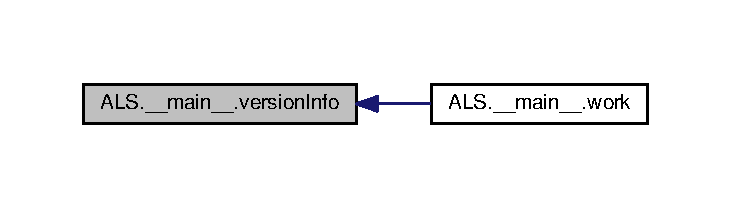
\includegraphics[width=350pt]{namespace_a_l_s_1_1____main_____af889c89bbfb175ee2f1ae173a2619946_icgraph}
\end{center}
\end{figure}


\hypertarget{namespace_a_l_s_1_1____main_____a4d3258d1ab0bf9938dc59b082a6d4ace}{\index{A\+L\+S\+::\+\_\+\+\_\+main\+\_\+\+\_\+@{A\+L\+S\+::\+\_\+\+\_\+main\+\_\+\+\_\+}!work@{work}}
\index{work@{work}!A\+L\+S\+::\+\_\+\+\_\+main\+\_\+\+\_\+@{A\+L\+S\+::\+\_\+\+\_\+main\+\_\+\+\_\+}}
\subsubsection[{work}]{\setlength{\rightskip}{0pt plus 5cm}def A\+L\+S.\+\_\+\+\_\+main\+\_\+\+\_\+.\+work (
\begin{DoxyParamCaption}
\item[{}]{inputfile}
\end{DoxyParamCaption}
)}}\label{namespace_a_l_s_1_1____main_____a4d3258d1ab0bf9938dc59b082a6d4ace}


Definition at line 51 of file \+\_\+\+\_\+main\+\_\+\+\_\+.\+py.



Here is the call graph for this function\+:
\nopagebreak
\begin{figure}[H]
\begin{center}
\leavevmode
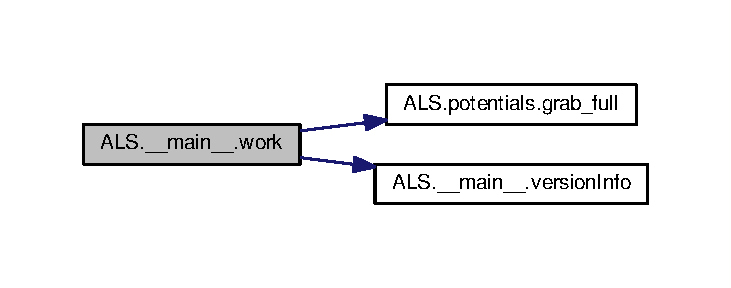
\includegraphics[width=350pt]{namespace_a_l_s_1_1____main_____a4d3258d1ab0bf9938dc59b082a6d4ace_cgraph}
\end{center}
\end{figure}




\subsection{Variable Documentation}
\hypertarget{namespace_a_l_s_1_1____main_____a261654567d538abacdaa62275d0839f9}{\index{A\+L\+S\+::\+\_\+\+\_\+main\+\_\+\+\_\+@{A\+L\+S\+::\+\_\+\+\_\+main\+\_\+\+\_\+}!\+\_\+\+\_\+author\+\_\+\+\_\+@{\+\_\+\+\_\+author\+\_\+\+\_\+}}
\index{\+\_\+\+\_\+author\+\_\+\+\_\+@{\+\_\+\+\_\+author\+\_\+\+\_\+}!A\+L\+S\+::\+\_\+\+\_\+main\+\_\+\+\_\+@{A\+L\+S\+::\+\_\+\+\_\+main\+\_\+\+\_\+}}
\subsubsection[{\+\_\+\+\_\+author\+\_\+\+\_\+}]{\setlength{\rightskip}{0pt plus 5cm}string A\+L\+S.\+\_\+\+\_\+main\+\_\+\+\_\+.\+\_\+\+\_\+author\+\_\+\+\_\+ = \char`\"{}Christian Delavier\char`\"{}}}\label{namespace_a_l_s_1_1____main_____a261654567d538abacdaa62275d0839f9}


Definition at line 11 of file \+\_\+\+\_\+main\+\_\+\+\_\+.\+py.

\hypertarget{namespace_a_l_s_1_1____main_____aa789b32fba45101c1352cea971ff935e}{\index{A\+L\+S\+::\+\_\+\+\_\+main\+\_\+\+\_\+@{A\+L\+S\+::\+\_\+\+\_\+main\+\_\+\+\_\+}!\+\_\+\+\_\+copyright\+\_\+\+\_\+@{\+\_\+\+\_\+copyright\+\_\+\+\_\+}}
\index{\+\_\+\+\_\+copyright\+\_\+\+\_\+@{\+\_\+\+\_\+copyright\+\_\+\+\_\+}!A\+L\+S\+::\+\_\+\+\_\+main\+\_\+\+\_\+@{A\+L\+S\+::\+\_\+\+\_\+main\+\_\+\+\_\+}}
\subsubsection[{\+\_\+\+\_\+copyright\+\_\+\+\_\+}]{\setlength{\rightskip}{0pt plus 5cm}string A\+L\+S.\+\_\+\+\_\+main\+\_\+\+\_\+.\+\_\+\+\_\+copyright\+\_\+\+\_\+ = \char`\"{}Theoretical Chemistry, University of Heidelberg\char`\"{}}}\label{namespace_a_l_s_1_1____main_____aa789b32fba45101c1352cea971ff935e}


Definition at line 12 of file \+\_\+\+\_\+main\+\_\+\+\_\+.\+py.

\hypertarget{namespace_a_l_s_1_1____main_____a0251675f23b74ea7707de3d1e69ce70f}{\index{A\+L\+S\+::\+\_\+\+\_\+main\+\_\+\+\_\+@{A\+L\+S\+::\+\_\+\+\_\+main\+\_\+\+\_\+}!\+\_\+\+\_\+email\+\_\+\+\_\+@{\+\_\+\+\_\+email\+\_\+\+\_\+}}
\index{\+\_\+\+\_\+email\+\_\+\+\_\+@{\+\_\+\+\_\+email\+\_\+\+\_\+}!A\+L\+S\+::\+\_\+\+\_\+main\+\_\+\+\_\+@{A\+L\+S\+::\+\_\+\+\_\+main\+\_\+\+\_\+}}
\subsubsection[{\+\_\+\+\_\+email\+\_\+\+\_\+}]{\setlength{\rightskip}{0pt plus 5cm}string A\+L\+S.\+\_\+\+\_\+main\+\_\+\+\_\+.\+\_\+\+\_\+email\+\_\+\+\_\+ = \char`\"{}delavier@stud.\+uni-\/heidelberg.\+de\char`\"{}}}\label{namespace_a_l_s_1_1____main_____a0251675f23b74ea7707de3d1e69ce70f}


Definition at line 15 of file \+\_\+\+\_\+main\+\_\+\+\_\+.\+py.

\hypertarget{namespace_a_l_s_1_1____main_____a5d02f90371afbc284e67f8b7627522bb}{\index{A\+L\+S\+::\+\_\+\+\_\+main\+\_\+\+\_\+@{A\+L\+S\+::\+\_\+\+\_\+main\+\_\+\+\_\+}!\+\_\+\+\_\+maintainer\+\_\+\+\_\+@{\+\_\+\+\_\+maintainer\+\_\+\+\_\+}}
\index{\+\_\+\+\_\+maintainer\+\_\+\+\_\+@{\+\_\+\+\_\+maintainer\+\_\+\+\_\+}!A\+L\+S\+::\+\_\+\+\_\+main\+\_\+\+\_\+@{A\+L\+S\+::\+\_\+\+\_\+main\+\_\+\+\_\+}}
\subsubsection[{\+\_\+\+\_\+maintainer\+\_\+\+\_\+}]{\setlength{\rightskip}{0pt plus 5cm}string A\+L\+S.\+\_\+\+\_\+main\+\_\+\+\_\+.\+\_\+\+\_\+maintainer\+\_\+\+\_\+ = \char`\"{}Christian Delavier\char`\"{}}}\label{namespace_a_l_s_1_1____main_____a5d02f90371afbc284e67f8b7627522bb}


Definition at line 14 of file \+\_\+\+\_\+main\+\_\+\+\_\+.\+py.

\hypertarget{namespace_a_l_s_1_1____main_____a6247bb85beb0771399c7ab617b11d74e}{\index{A\+L\+S\+::\+\_\+\+\_\+main\+\_\+\+\_\+@{A\+L\+S\+::\+\_\+\+\_\+main\+\_\+\+\_\+}!\+\_\+\+\_\+status\+\_\+\+\_\+@{\+\_\+\+\_\+status\+\_\+\+\_\+}}
\index{\+\_\+\+\_\+status\+\_\+\+\_\+@{\+\_\+\+\_\+status\+\_\+\+\_\+}!A\+L\+S\+::\+\_\+\+\_\+main\+\_\+\+\_\+@{A\+L\+S\+::\+\_\+\+\_\+main\+\_\+\+\_\+}}
\subsubsection[{\+\_\+\+\_\+status\+\_\+\+\_\+}]{\setlength{\rightskip}{0pt plus 5cm}string A\+L\+S.\+\_\+\+\_\+main\+\_\+\+\_\+.\+\_\+\+\_\+status\+\_\+\+\_\+ = \char`\"{}Development\char`\"{}}}\label{namespace_a_l_s_1_1____main_____a6247bb85beb0771399c7ab617b11d74e}


Definition at line 16 of file \+\_\+\+\_\+main\+\_\+\+\_\+.\+py.

\hypertarget{namespace_a_l_s_1_1____main_____aff934e6ec8e8870ccc1356e92dd9f909}{\index{A\+L\+S\+::\+\_\+\+\_\+main\+\_\+\+\_\+@{A\+L\+S\+::\+\_\+\+\_\+main\+\_\+\+\_\+}!\+\_\+\+\_\+version\+\_\+\+\_\+@{\+\_\+\+\_\+version\+\_\+\+\_\+}}
\index{\+\_\+\+\_\+version\+\_\+\+\_\+@{\+\_\+\+\_\+version\+\_\+\+\_\+}!A\+L\+S\+::\+\_\+\+\_\+main\+\_\+\+\_\+@{A\+L\+S\+::\+\_\+\+\_\+main\+\_\+\+\_\+}}
\subsubsection[{\+\_\+\+\_\+version\+\_\+\+\_\+}]{\setlength{\rightskip}{0pt plus 5cm}string A\+L\+S.\+\_\+\+\_\+main\+\_\+\+\_\+.\+\_\+\+\_\+version\+\_\+\+\_\+ = \char`\"{}0.\+1\char`\"{}}}\label{namespace_a_l_s_1_1____main_____aff934e6ec8e8870ccc1356e92dd9f909}


Definition at line 13 of file \+\_\+\+\_\+main\+\_\+\+\_\+.\+py.

\hypertarget{namespace_a_l_s_1_1____main_____a3865f3dc40606d46564c911de0639778}{\index{A\+L\+S\+::\+\_\+\+\_\+main\+\_\+\+\_\+@{A\+L\+S\+::\+\_\+\+\_\+main\+\_\+\+\_\+}!copyright@{copyright}}
\index{copyright@{copyright}!A\+L\+S\+::\+\_\+\+\_\+main\+\_\+\+\_\+@{A\+L\+S\+::\+\_\+\+\_\+main\+\_\+\+\_\+}}
\subsubsection[{copyright}]{\setlength{\rightskip}{0pt plus 5cm}A\+L\+S.\+\_\+\+\_\+main\+\_\+\+\_\+.\+copyright = {\bf \+\_\+\+\_\+email\+\_\+\+\_\+})}}\label{namespace_a_l_s_1_1____main_____a3865f3dc40606d46564c911de0639778}


Definition at line 142 of file \+\_\+\+\_\+main\+\_\+\+\_\+.\+py.

\hypertarget{namespace_a_l_s_1_1____main_____aa5b527ae9e22a81c1b94a9de1950f075}{\index{A\+L\+S\+::\+\_\+\+\_\+main\+\_\+\+\_\+@{A\+L\+S\+::\+\_\+\+\_\+main\+\_\+\+\_\+}!file@{file}}
\index{file@{file}!A\+L\+S\+::\+\_\+\+\_\+main\+\_\+\+\_\+@{A\+L\+S\+::\+\_\+\+\_\+main\+\_\+\+\_\+}}
\subsubsection[{file}]{\setlength{\rightskip}{0pt plus 5cm}list A\+L\+S.\+\_\+\+\_\+main\+\_\+\+\_\+.\+file = \mbox{[}f for f in {\bf files} if '.inp' in f\mbox{]}}}\label{namespace_a_l_s_1_1____main_____aa5b527ae9e22a81c1b94a9de1950f075}


Definition at line 149 of file \+\_\+\+\_\+main\+\_\+\+\_\+.\+py.

\hypertarget{namespace_a_l_s_1_1____main_____a0d16fe12e38a76b5e5c925f6f685b55b}{\index{A\+L\+S\+::\+\_\+\+\_\+main\+\_\+\+\_\+@{A\+L\+S\+::\+\_\+\+\_\+main\+\_\+\+\_\+}!files@{files}}
\index{files@{files}!A\+L\+S\+::\+\_\+\+\_\+main\+\_\+\+\_\+@{A\+L\+S\+::\+\_\+\+\_\+main\+\_\+\+\_\+}}
\subsubsection[{files}]{\setlength{\rightskip}{0pt plus 5cm}tuple A\+L\+S.\+\_\+\+\_\+main\+\_\+\+\_\+.\+files = os.\+listdir('.')}}\label{namespace_a_l_s_1_1____main_____a0d16fe12e38a76b5e5c925f6f685b55b}


Definition at line 148 of file \+\_\+\+\_\+main\+\_\+\+\_\+.\+py.

\hypertarget{namespace_a_l_s_1_1____main_____a5aa0409d9d67fa40ab9ea2c561dacb51}{\index{A\+L\+S\+::\+\_\+\+\_\+main\+\_\+\+\_\+@{A\+L\+S\+::\+\_\+\+\_\+main\+\_\+\+\_\+}!idx@{idx}}
\index{idx@{idx}!A\+L\+S\+::\+\_\+\+\_\+main\+\_\+\+\_\+@{A\+L\+S\+::\+\_\+\+\_\+main\+\_\+\+\_\+}}
\subsubsection[{idx}]{\setlength{\rightskip}{0pt plus 5cm}tuple A\+L\+S.\+\_\+\+\_\+main\+\_\+\+\_\+.\+idx = input('Choose input by index or abort with n\+:')}}\label{namespace_a_l_s_1_1____main_____a5aa0409d9d67fa40ab9ea2c561dacb51}


Definition at line 162 of file \+\_\+\+\_\+main\+\_\+\+\_\+.\+py.

\hypertarget{namespace_a_l_s_1_1____main_____aa9daddee8a81563388242dfedc17c588}{\index{A\+L\+S\+::\+\_\+\+\_\+main\+\_\+\+\_\+@{A\+L\+S\+::\+\_\+\+\_\+main\+\_\+\+\_\+}!initialized@{initialized}}
\index{initialized@{initialized}!A\+L\+S\+::\+\_\+\+\_\+main\+\_\+\+\_\+@{A\+L\+S\+::\+\_\+\+\_\+main\+\_\+\+\_\+}}
\subsubsection[{initialized}]{\setlength{\rightskip}{0pt plus 5cm}A\+L\+S.\+\_\+\+\_\+main\+\_\+\+\_\+.\+initialized = False}}\label{namespace_a_l_s_1_1____main_____aa9daddee8a81563388242dfedc17c588}


Definition at line 144 of file \+\_\+\+\_\+main\+\_\+\+\_\+.\+py.

\hypertarget{namespace_a_l_s_1_1____main_____ab3aa61ab51823df019a351f6bb82b138}{\index{A\+L\+S\+::\+\_\+\+\_\+main\+\_\+\+\_\+@{A\+L\+S\+::\+\_\+\+\_\+main\+\_\+\+\_\+}!Obj@{Obj}}
\index{Obj@{Obj}!A\+L\+S\+::\+\_\+\+\_\+main\+\_\+\+\_\+@{A\+L\+S\+::\+\_\+\+\_\+main\+\_\+\+\_\+}}
\subsubsection[{Obj}]{\setlength{\rightskip}{0pt plus 5cm}A\+L\+S.\+\_\+\+\_\+main\+\_\+\+\_\+.\+Obj = False}}\label{namespace_a_l_s_1_1____main_____ab3aa61ab51823df019a351f6bb82b138}


Definition at line 145 of file \+\_\+\+\_\+main\+\_\+\+\_\+.\+py.

\hypertarget{namespace_a_l_s_1_1____main_____a610b87b76246245771ea935477540795}{\index{A\+L\+S\+::\+\_\+\+\_\+main\+\_\+\+\_\+@{A\+L\+S\+::\+\_\+\+\_\+main\+\_\+\+\_\+}!Object@{Object}}
\index{Object@{Object}!A\+L\+S\+::\+\_\+\+\_\+main\+\_\+\+\_\+@{A\+L\+S\+::\+\_\+\+\_\+main\+\_\+\+\_\+}}
\subsubsection[{Object}]{\setlength{\rightskip}{0pt plus 5cm}tuple A\+L\+S.\+\_\+\+\_\+main\+\_\+\+\_\+.\+Object}}\label{namespace_a_l_s_1_1____main_____a610b87b76246245771ea935477540795}
{\bfseries Initial value\+:}
\begin{DoxyCode}
1 = \hyperlink{class_a_l_s_1_1_a_l_sclass_1_1_a_l_s_c_p_d}{ALSCPD}(filename, pot, rank, func1D=h2o1D, func2D=h2o2D,\(\backslash\)
2                                     grids=grids, nsmpl=nsmpl, presmpl=sampl)
\end{DoxyCode}


Definition at line 196 of file \+\_\+\+\_\+main\+\_\+\+\_\+.\+py.

\hypertarget{namespace_a_l_s_1_1____main_____ac0e196b18c2c5ce3593885fa2cd7174c}{\index{A\+L\+S\+::\+\_\+\+\_\+main\+\_\+\+\_\+@{A\+L\+S\+::\+\_\+\+\_\+main\+\_\+\+\_\+}!pot@{pot}}
\index{pot@{pot}!A\+L\+S\+::\+\_\+\+\_\+main\+\_\+\+\_\+@{A\+L\+S\+::\+\_\+\+\_\+main\+\_\+\+\_\+}}
\subsubsection[{pot}]{\setlength{\rightskip}{0pt plus 5cm}tuple A\+L\+S.\+\_\+\+\_\+main\+\_\+\+\_\+.\+pot = geth2o($\ast$grids)}}\label{namespace_a_l_s_1_1____main_____ac0e196b18c2c5ce3593885fa2cd7174c}


Definition at line 182 of file \+\_\+\+\_\+main\+\_\+\+\_\+.\+py.


\hypertarget{namespace_a_l_s_1_1_a_l_s1_d}{\section{A\+L\+S.\+A\+L\+S1\+D Namespace Reference}
\label{namespace_a_l_s_1_1_a_l_s1_d}\index{A\+L\+S.\+A\+L\+S1\+D@{A\+L\+S.\+A\+L\+S1\+D}}
}
\subsection*{Functions}
\begin{DoxyCompactItemize}
\item 
def \hyperlink{namespace_a_l_s_1_1_a_l_s1_d_a32c360de0d2968c3420aba6db27aab03}{init\+A\+L\+S}
\item 
def \hyperlink{namespace_a_l_s_1_1_a_l_s1_d_a2fd6554e1ae1c9cb742260746fd46bcb}{get\+\_\+norm}
\item 
def \hyperlink{namespace_a_l_s_1_1_a_l_s1_d_ac420366e2c70d0554cf7a8fde0b93e3e}{get\+\_\+sigmas}
\item 
def \hyperlink{namespace_a_l_s_1_1_a_l_s1_d_a994f6e3fde98eeeeb090fd856c2e4844}{update\+\_\+sigma}
\item 
def \hyperlink{namespace_a_l_s_1_1_a_l_s1_d_a36b5c4ceb1ab2bd22d085716e5cf18f4}{assemble\+\_\+\+S}
\item 
def \hyperlink{namespace_a_l_s_1_1_a_l_s1_d_ac09997ab1bf46477a1a0c4e5cb8411b8}{get\+\_\+b\+\_\+ein}
\item 
def \hyperlink{namespace_a_l_s_1_1_a_l_s1_d_a964d2ee3d2fa472027342adbb4fa7c2e}{solve\+\_\+linear}
\item 
def \hyperlink{namespace_a_l_s_1_1_a_l_s1_d_a0e620f84229f80936a74dadc3ab16675}{geterrorleft}
\item 
def \hyperlink{namespace_a_l_s_1_1_a_l_s1_d_af57f376f29c970d07bcb4ae6d4b287fe}{geterrorright}
\item 
def \hyperlink{namespace_a_l_s_1_1_a_l_s1_d_a49e8fa6e552e24a4ce1b92168d08933a}{get\+\_\+rmse}
\item 
def \hyperlink{namespace_a_l_s_1_1_a_l_s1_d_a9eaea1906f96507bb770b52ebbe77c82}{get\+\_\+update}
\end{DoxyCompactItemize}
\subsection*{Variables}
\begin{DoxyCompactItemize}
\item 
float \hyperlink{namespace_a_l_s_1_1_a_l_s1_d_a6225364b4130ce75f06fc87c2741007f}{au2ic} = 219474.\+63137
\end{DoxyCompactItemize}


\subsection{Function Documentation}
\hypertarget{namespace_a_l_s_1_1_a_l_s1_d_a36b5c4ceb1ab2bd22d085716e5cf18f4}{\index{A\+L\+S\+::\+A\+L\+S1\+D@{A\+L\+S\+::\+A\+L\+S1\+D}!assemble\+\_\+\+S@{assemble\+\_\+\+S}}
\index{assemble\+\_\+\+S@{assemble\+\_\+\+S}!A\+L\+S\+::\+A\+L\+S1\+D@{A\+L\+S\+::\+A\+L\+S1\+D}}
\subsubsection[{assemble\+\_\+\+S}]{\setlength{\rightskip}{0pt plus 5cm}def A\+L\+S.\+A\+L\+S1\+D.\+assemble\+\_\+\+S (
\begin{DoxyParamCaption}
\item[{}]{sigma\+\_\+list, }
\item[{}]{hole\+\_\+index = {\ttfamily None}}
\end{DoxyParamCaption}
)}}\label{namespace_a_l_s_1_1_a_l_s1_d_a36b5c4ceb1ab2bd22d085716e5cf18f4}
\begin{DoxyVerb}Assemble the overlap matrix from a given list of sigmas. One can choose to neglect one sigma.

[Args]:
        sigma_list[list]: List containing the individual terms for all the SPP.
        hole_index[int]: Index of the sigma to be neglected. Default=None returns full overlap matrix.
        
[Returns]:
        [Array]: Array containing the overlap matrix for a given set of SPP.\end{DoxyVerb}
 

Definition at line 94 of file A\+L\+S1\+D.\+py.



Here is the caller graph for this function\+:
\nopagebreak
\begin{figure}[H]
\begin{center}
\leavevmode
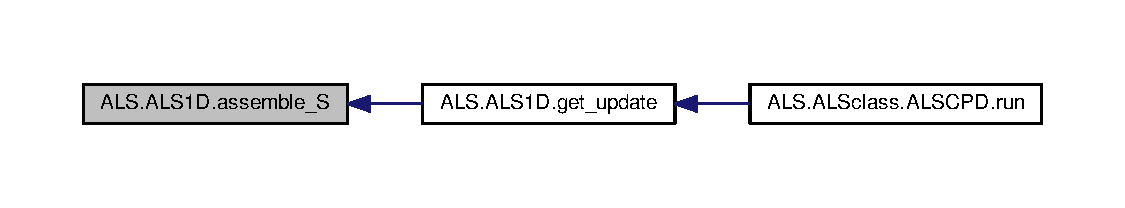
\includegraphics[width=350pt]{namespace_a_l_s_1_1_a_l_s1_d_a36b5c4ceb1ab2bd22d085716e5cf18f4_icgraph}
\end{center}
\end{figure}


\hypertarget{namespace_a_l_s_1_1_a_l_s1_d_ac09997ab1bf46477a1a0c4e5cb8411b8}{\index{A\+L\+S\+::\+A\+L\+S1\+D@{A\+L\+S\+::\+A\+L\+S1\+D}!get\+\_\+b\+\_\+ein@{get\+\_\+b\+\_\+ein}}
\index{get\+\_\+b\+\_\+ein@{get\+\_\+b\+\_\+ein}!A\+L\+S\+::\+A\+L\+S1\+D@{A\+L\+S\+::\+A\+L\+S1\+D}}
\subsubsection[{get\+\_\+b\+\_\+ein}]{\setlength{\rightskip}{0pt plus 5cm}def A\+L\+S.\+A\+L\+S1\+D.\+get\+\_\+b\+\_\+ein (
\begin{DoxyParamCaption}
\item[{}]{V, }
\item[{}]{nu\+\_\+store, }
\item[{}]{hole\+\_\+index}
\end{DoxyParamCaption}
)}}\label{namespace_a_l_s_1_1_a_l_s1_d_ac09997ab1bf46477a1a0c4e5cb8411b8}
\begin{DoxyVerb}Function to iteratively create input for the np.einsum routine to contract a given tensor with given
set of SPP for all DOF except one indicated.

[Args]:
        V[array]: The exact tensor to be contracted with shape (N0, N1, N2,... Nf).
        nu_store[list]: List of the SPP with index running over the DOF in shape (r,N).
        hole_index[int]: Index of the DOF to be neglected with SPP of shape (r,Nk).
        
[Returns]:
        [Array]: Contracted tensor with shape (r,Nk).
        
-tested for up to 6D potential.\end{DoxyVerb}
 

Definition at line 127 of file A\+L\+S1\+D.\+py.



Here is the caller graph for this function\+:
\nopagebreak
\begin{figure}[H]
\begin{center}
\leavevmode
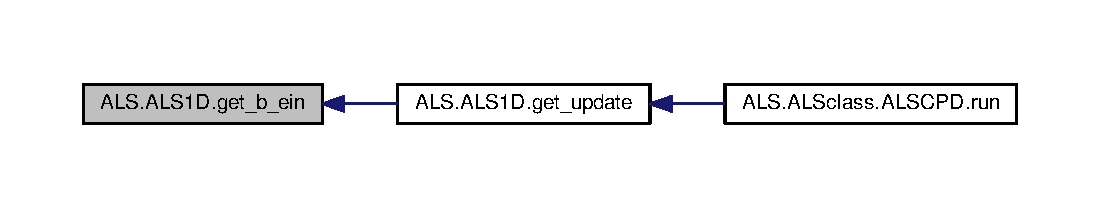
\includegraphics[width=350pt]{namespace_a_l_s_1_1_a_l_s1_d_ac09997ab1bf46477a1a0c4e5cb8411b8_icgraph}
\end{center}
\end{figure}


\hypertarget{namespace_a_l_s_1_1_a_l_s1_d_a2fd6554e1ae1c9cb742260746fd46bcb}{\index{A\+L\+S\+::\+A\+L\+S1\+D@{A\+L\+S\+::\+A\+L\+S1\+D}!get\+\_\+norm@{get\+\_\+norm}}
\index{get\+\_\+norm@{get\+\_\+norm}!A\+L\+S\+::\+A\+L\+S1\+D@{A\+L\+S\+::\+A\+L\+S1\+D}}
\subsubsection[{get\+\_\+norm}]{\setlength{\rightskip}{0pt plus 5cm}def A\+L\+S.\+A\+L\+S1\+D.\+get\+\_\+norm (
\begin{DoxyParamCaption}
\item[{}]{nu\+\_\+k}
\end{DoxyParamCaption}
)}}\label{namespace_a_l_s_1_1_a_l_s1_d_a2fd6554e1ae1c9cb742260746fd46bcb}
\begin{DoxyVerb}Function to get the new weights by normalizing rows of the solution to the
linear equation of ALS.

[Args]:
        x_k[array]: (r,Nk) shaped array containing the new SPP resulting from solving
                    the linear equation.
                    
[Returns]:
        [array]: array of the new weights in shape (r).
        [array]: array of the new normalized SPP in shape (r,N).\end{DoxyVerb}
 

Definition at line 35 of file A\+L\+S1\+D.\+py.



Here is the caller graph for this function\+:
\nopagebreak
\begin{figure}[H]
\begin{center}
\leavevmode
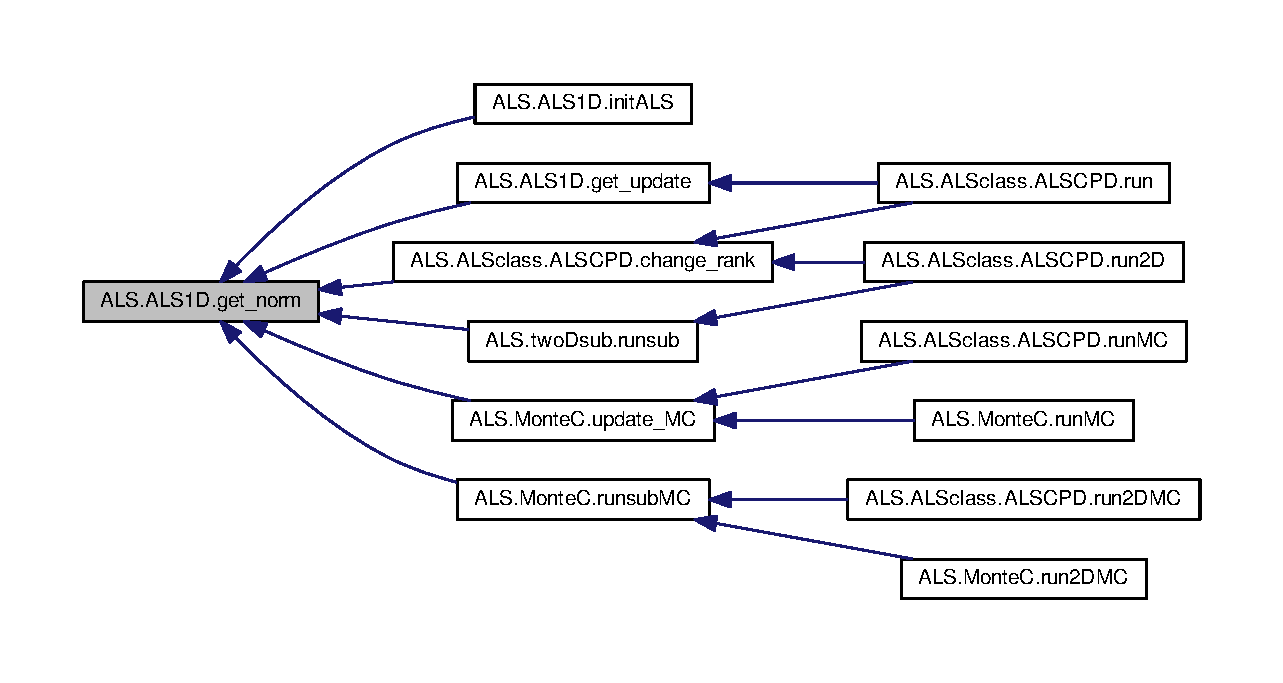
\includegraphics[width=350pt]{namespace_a_l_s_1_1_a_l_s1_d_a2fd6554e1ae1c9cb742260746fd46bcb_icgraph}
\end{center}
\end{figure}


\hypertarget{namespace_a_l_s_1_1_a_l_s1_d_a49e8fa6e552e24a4ce1b92168d08933a}{\index{A\+L\+S\+::\+A\+L\+S1\+D@{A\+L\+S\+::\+A\+L\+S1\+D}!get\+\_\+rmse@{get\+\_\+rmse}}
\index{get\+\_\+rmse@{get\+\_\+rmse}!A\+L\+S\+::\+A\+L\+S1\+D@{A\+L\+S\+::\+A\+L\+S1\+D}}
\subsubsection[{get\+\_\+rmse}]{\setlength{\rightskip}{0pt plus 5cm}def A\+L\+S.\+A\+L\+S1\+D.\+get\+\_\+rmse (
\begin{DoxyParamCaption}
\item[{}]{er1, }
\item[{}]{er2}
\end{DoxyParamCaption}
)}}\label{namespace_a_l_s_1_1_a_l_s1_d_a49e8fa6e552e24a4ce1b92168d08933a}
\begin{DoxyVerb}Get the RMSE of the complete 1D ALS functional in cm-1.

[Args]:
    er1[float]: MSE of the left hand side of the ALS functional.
    er2[float]: MSE of the right hand side of the ALS functional.
    
[Returns]:
    [float]: RMSE of the complete ALS functional in cm-1.\end{DoxyVerb}
 

Definition at line 256 of file A\+L\+S1\+D.\+py.



Here is the caller graph for this function\+:
\nopagebreak
\begin{figure}[H]
\begin{center}
\leavevmode
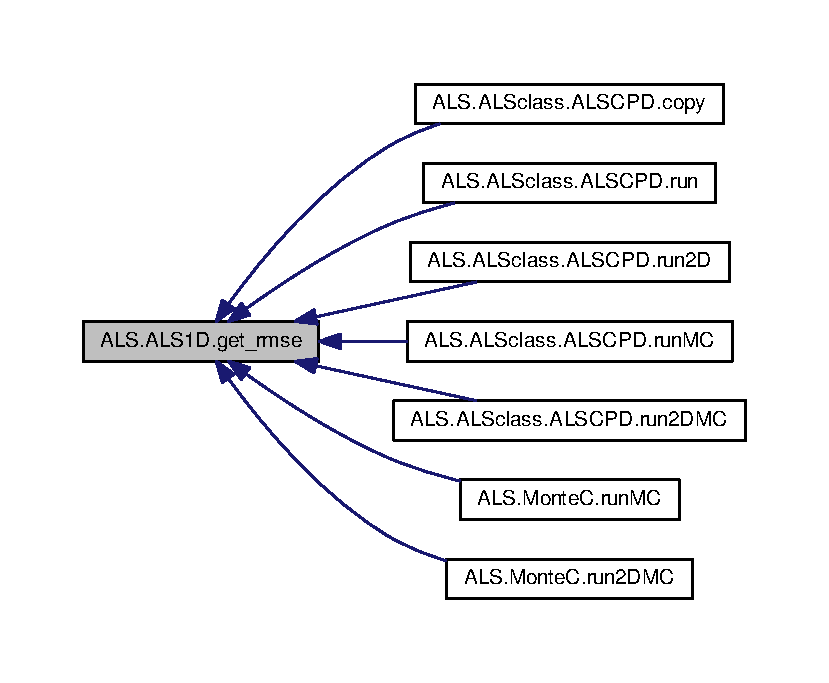
\includegraphics[width=350pt]{namespace_a_l_s_1_1_a_l_s1_d_a49e8fa6e552e24a4ce1b92168d08933a_icgraph}
\end{center}
\end{figure}


\hypertarget{namespace_a_l_s_1_1_a_l_s1_d_ac420366e2c70d0554cf7a8fde0b93e3e}{\index{A\+L\+S\+::\+A\+L\+S1\+D@{A\+L\+S\+::\+A\+L\+S1\+D}!get\+\_\+sigmas@{get\+\_\+sigmas}}
\index{get\+\_\+sigmas@{get\+\_\+sigmas}!A\+L\+S\+::\+A\+L\+S1\+D@{A\+L\+S\+::\+A\+L\+S1\+D}}
\subsubsection[{get\+\_\+sigmas}]{\setlength{\rightskip}{0pt plus 5cm}def A\+L\+S.\+A\+L\+S1\+D.\+get\+\_\+sigmas (
\begin{DoxyParamCaption}
\item[{}]{nu\+\_\+store}
\end{DoxyParamCaption}
)}}\label{namespace_a_l_s_1_1_a_l_s1_d_ac420366e2c70d0554cf7a8fde0b93e3e}
\begin{DoxyVerb}Get the matrices which will be multiplied to result in the overlap matrix.

[Args]:
        nu_store[array]: Data structure containing the SPP for each DOF in shape (r,Nk), index running over
                        the DOF.
[Returns]:
        [List]: List containing all the sigmas (SPP @ {SPP}transposed) in shape (r,r).\end{DoxyVerb}
 

Definition at line 62 of file A\+L\+S1\+D.\+py.



Here is the caller graph for this function\+:
\nopagebreak
\begin{figure}[H]
\begin{center}
\leavevmode
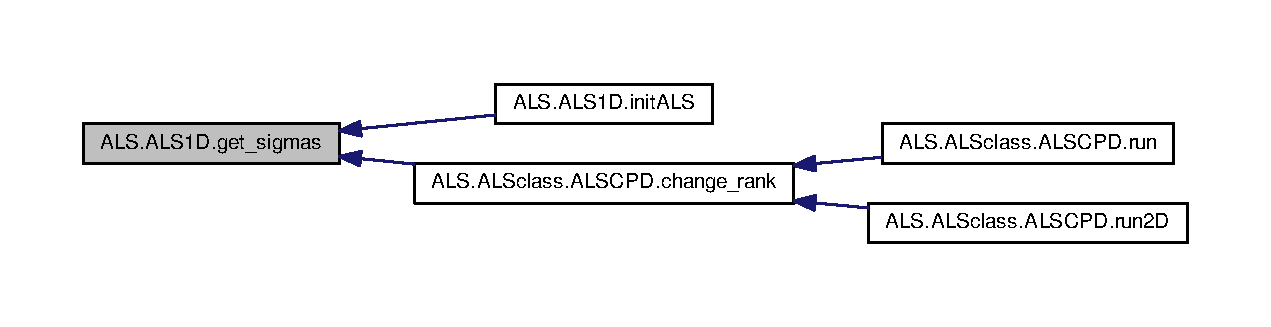
\includegraphics[width=350pt]{namespace_a_l_s_1_1_a_l_s1_d_ac420366e2c70d0554cf7a8fde0b93e3e_icgraph}
\end{center}
\end{figure}


\hypertarget{namespace_a_l_s_1_1_a_l_s1_d_a9eaea1906f96507bb770b52ebbe77c82}{\index{A\+L\+S\+::\+A\+L\+S1\+D@{A\+L\+S\+::\+A\+L\+S1\+D}!get\+\_\+update@{get\+\_\+update}}
\index{get\+\_\+update@{get\+\_\+update}!A\+L\+S\+::\+A\+L\+S1\+D@{A\+L\+S\+::\+A\+L\+S1\+D}}
\subsubsection[{get\+\_\+update}]{\setlength{\rightskip}{0pt plus 5cm}def A\+L\+S.\+A\+L\+S1\+D.\+get\+\_\+update (
\begin{DoxyParamCaption}
\item[{}]{v\+\_\+ex, }
\item[{}]{nu\+\_\+r, }
\item[{}]{sigmas, }
\item[{}]{k, }
\item[{}]{prec = {\ttfamily None}}
\end{DoxyParamCaption}
)}}\label{namespace_a_l_s_1_1_a_l_s1_d_a9eaea1906f96507bb770b52ebbe77c82}
\begin{DoxyVerb}Function to get the updated weights and the normalized new nu for one DOF.

[Args]:
        v_ex[array]: Array of shape (N1, N2,..., Nf) containing the exact potential.
        nu_r[list]: List of the SPP for all DOF given in shape (r,N).
        sigmas[list]: List of the sigmas to build the S-matrix. (Sigma_k = nu_r[k]@nu_r[k].T).
        k[int]: Index of the current DOF to update.
        
[Returns]:
        [Array]: (r) shaped array containing the new weights.
        [array]: (r,Nk) shaped array containing the new normalized SPP.\end{DoxyVerb}
 

Definition at line 268 of file A\+L\+S1\+D.\+py.



Here is the call graph for this function\+:
\nopagebreak
\begin{figure}[H]
\begin{center}
\leavevmode
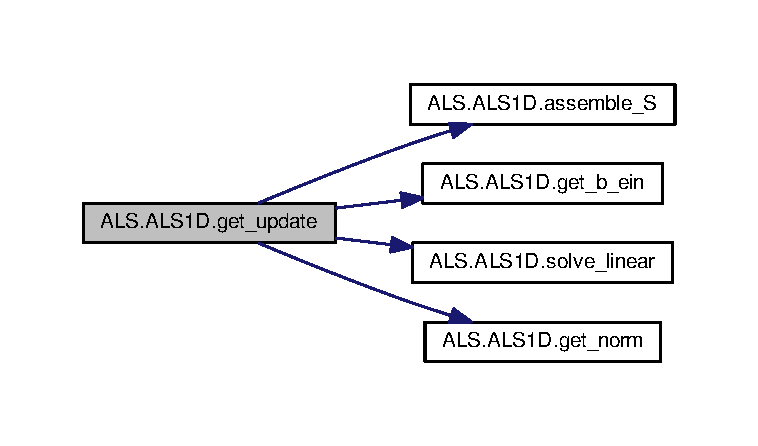
\includegraphics[width=350pt]{namespace_a_l_s_1_1_a_l_s1_d_a9eaea1906f96507bb770b52ebbe77c82_cgraph}
\end{center}
\end{figure}




Here is the caller graph for this function\+:
\nopagebreak
\begin{figure}[H]
\begin{center}
\leavevmode
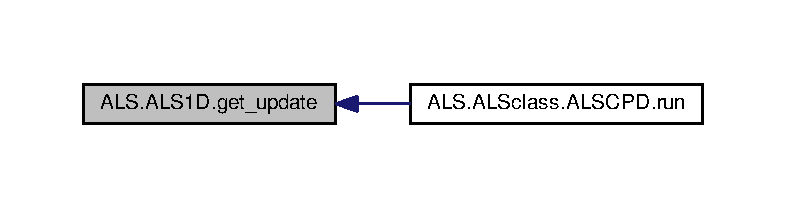
\includegraphics[width=350pt]{namespace_a_l_s_1_1_a_l_s1_d_a9eaea1906f96507bb770b52ebbe77c82_icgraph}
\end{center}
\end{figure}


\hypertarget{namespace_a_l_s_1_1_a_l_s1_d_a0e620f84229f80936a74dadc3ab16675}{\index{A\+L\+S\+::\+A\+L\+S1\+D@{A\+L\+S\+::\+A\+L\+S1\+D}!geterrorleft@{geterrorleft}}
\index{geterrorleft@{geterrorleft}!A\+L\+S\+::\+A\+L\+S1\+D@{A\+L\+S\+::\+A\+L\+S1\+D}}
\subsubsection[{geterrorleft}]{\setlength{\rightskip}{0pt plus 5cm}def A\+L\+S.\+A\+L\+S1\+D.\+geterrorleft (
\begin{DoxyParamCaption}
\item[{}]{V\+\_\+ex, }
\item[{}]{weights, }
\item[{}]{nu\+\_\+list}
\end{DoxyParamCaption}
)}}\label{namespace_a_l_s_1_1_a_l_s1_d_a0e620f84229f80936a74dadc3ab16675}
\begin{DoxyVerb}Get the mean square error between the initial tensor and the current tensor which will
be rebuild from factor matrices given as shape (r,N).

[Args]:
        V_ex[array]: Exact tensor of shape (N1, N2,..., Nf).
        weights[array]: shape (r) array with the weights for the reconstruction of the current
                    tensor.
        nu_list[list]: List of the factor matrices of shape (r,N) to rebuild the current tensor.
        
[Returns]:
        [float]: Mean square error [cm-1] between initial tensor and rebuild tensor.\end{DoxyVerb}
 

Definition at line 214 of file A\+L\+S1\+D.\+py.



Here is the caller graph for this function\+:
\nopagebreak
\begin{figure}[H]
\begin{center}
\leavevmode
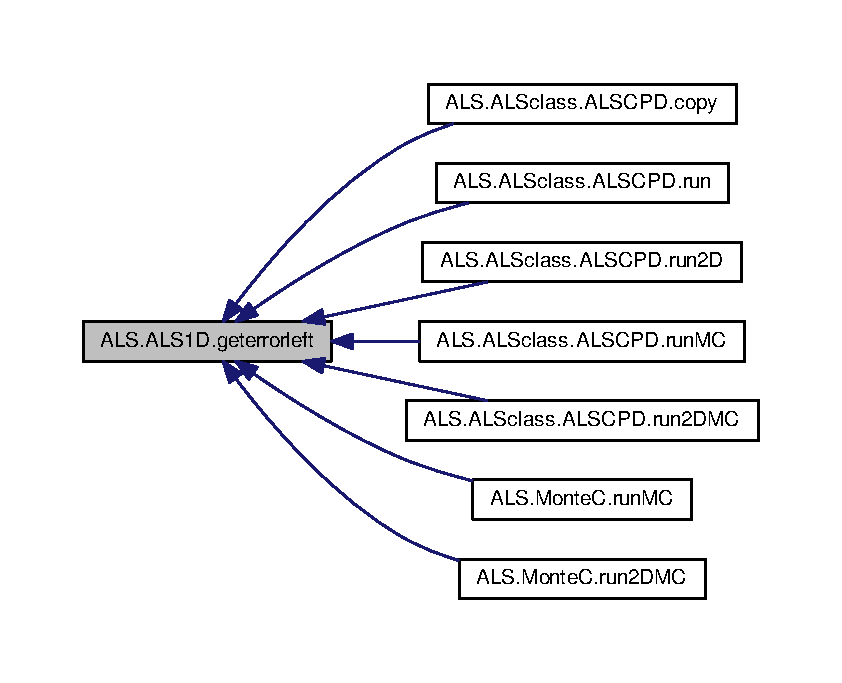
\includegraphics[width=350pt]{namespace_a_l_s_1_1_a_l_s1_d_a0e620f84229f80936a74dadc3ab16675_icgraph}
\end{center}
\end{figure}


\hypertarget{namespace_a_l_s_1_1_a_l_s1_d_af57f376f29c970d07bcb4ae6d4b287fe}{\index{A\+L\+S\+::\+A\+L\+S1\+D@{A\+L\+S\+::\+A\+L\+S1\+D}!geterrorright@{geterrorright}}
\index{geterrorright@{geterrorright}!A\+L\+S\+::\+A\+L\+S1\+D@{A\+L\+S\+::\+A\+L\+S1\+D}}
\subsubsection[{geterrorright}]{\setlength{\rightskip}{0pt plus 5cm}def A\+L\+S.\+A\+L\+S1\+D.\+geterrorright (
\begin{DoxyParamCaption}
\item[{}]{v\+\_\+ex, }
\item[{}]{c\+\_\+r, }
\item[{}]{prec = {\ttfamily None}}
\end{DoxyParamCaption}
)}}\label{namespace_a_l_s_1_1_a_l_s1_d_af57f376f29c970d07bcb4ae6d4b287fe}
\begin{DoxyVerb}Get the mean squared error for the right hand side of the ALS functional given as the 
root of the sum over the squared weights multiplied by the regularization devided by the number of weights.

[Args]:
        c_r[array]: (r) shaped array containing the current weights.
        prec[float]: Gives the epsilon for the regularization, standard is root of machine precision for
                float (~1E-8).
                
[Returns]:
        [float]: The mean squared error [cm-1] for the right hand side ALS functional.\end{DoxyVerb}
 

Definition at line 238 of file A\+L\+S1\+D.\+py.



Here is the caller graph for this function\+:
\nopagebreak
\begin{figure}[H]
\begin{center}
\leavevmode
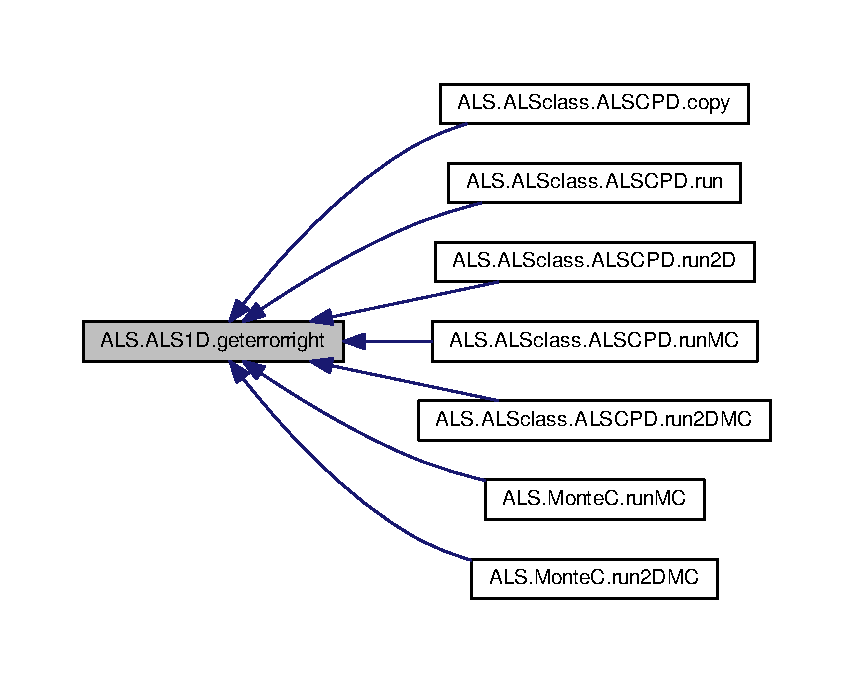
\includegraphics[width=350pt]{namespace_a_l_s_1_1_a_l_s1_d_af57f376f29c970d07bcb4ae6d4b287fe_icgraph}
\end{center}
\end{figure}


\hypertarget{namespace_a_l_s_1_1_a_l_s1_d_a32c360de0d2968c3420aba6db27aab03}{\index{A\+L\+S\+::\+A\+L\+S1\+D@{A\+L\+S\+::\+A\+L\+S1\+D}!init\+A\+L\+S@{init\+A\+L\+S}}
\index{init\+A\+L\+S@{init\+A\+L\+S}!A\+L\+S\+::\+A\+L\+S1\+D@{A\+L\+S\+::\+A\+L\+S1\+D}}
\subsubsection[{init\+A\+L\+S}]{\setlength{\rightskip}{0pt plus 5cm}def A\+L\+S.\+A\+L\+S1\+D.\+init\+A\+L\+S (
\begin{DoxyParamCaption}
\item[{}]{r, }
\item[{}]{point\+\_\+list}
\end{DoxyParamCaption}
)}}\label{namespace_a_l_s_1_1_a_l_s1_d_a32c360de0d2968c3420aba6db27aab03}
\begin{DoxyVerb}Function to initialize the ALS.

[Args]:
        r[int]: Current expansion rank in CPD.
        point_list[list]: List containing the number of grid points along each
                axis of the full tensor.
                
[Returns]:
        c_r_init[array]: Array of shape (r) containing zeros, the initial weights.
        nu_r_list_init[list]: List containing the random normalized SPP of shape (r,Nk) for
                all DOF.\end{DoxyVerb}
 

Definition at line 11 of file A\+L\+S1\+D.\+py.



Here is the call graph for this function\+:
\nopagebreak
\begin{figure}[H]
\begin{center}
\leavevmode
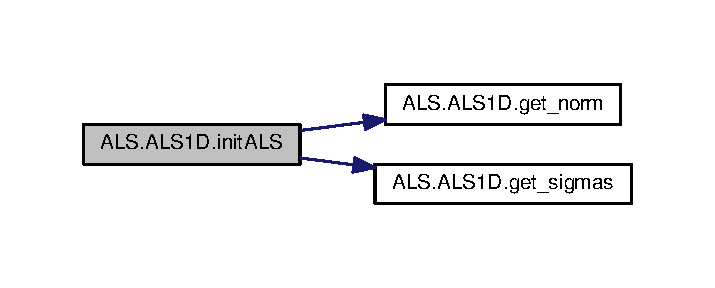
\includegraphics[width=343pt]{namespace_a_l_s_1_1_a_l_s1_d_a32c360de0d2968c3420aba6db27aab03_cgraph}
\end{center}
\end{figure}


\hypertarget{namespace_a_l_s_1_1_a_l_s1_d_a964d2ee3d2fa472027342adbb4fa7c2e}{\index{A\+L\+S\+::\+A\+L\+S1\+D@{A\+L\+S\+::\+A\+L\+S1\+D}!solve\+\_\+linear@{solve\+\_\+linear}}
\index{solve\+\_\+linear@{solve\+\_\+linear}!A\+L\+S\+::\+A\+L\+S1\+D@{A\+L\+S\+::\+A\+L\+S1\+D}}
\subsubsection[{solve\+\_\+linear}]{\setlength{\rightskip}{0pt plus 5cm}def A\+L\+S.\+A\+L\+S1\+D.\+solve\+\_\+linear (
\begin{DoxyParamCaption}
\item[{}]{S, }
\item[{}]{b, }
\item[{}]{prec = {\ttfamily None}}
\end{DoxyParamCaption}
)}}\label{namespace_a_l_s_1_1_a_l_s1_d_a964d2ee3d2fa472027342adbb4fa7c2e}
\begin{DoxyVerb}A function to solve the linear equation in 1D ALS.

[Args]:
        S[array]: (r,r) array containing the S_k k-hole overlap matrix.
        b[array]: (r,Nk) array containing the b_k k-hole overlap with the
                    exact tensor.
        prec[float]: Gives the epsilon for the regularization, standard is root of machine precision for
                float (~1E-8).
                
[Returns]:
        [array]: (r,Nk) array containing the new nu_k non-normalized.\end{DoxyVerb}
 

Definition at line 191 of file A\+L\+S1\+D.\+py.



Here is the caller graph for this function\+:
\nopagebreak
\begin{figure}[H]
\begin{center}
\leavevmode
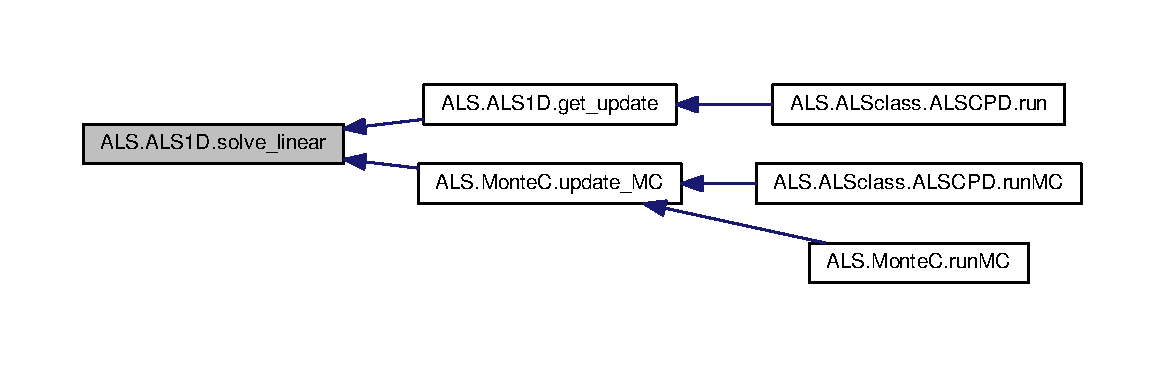
\includegraphics[width=350pt]{namespace_a_l_s_1_1_a_l_s1_d_a964d2ee3d2fa472027342adbb4fa7c2e_icgraph}
\end{center}
\end{figure}


\hypertarget{namespace_a_l_s_1_1_a_l_s1_d_a994f6e3fde98eeeeb090fd856c2e4844}{\index{A\+L\+S\+::\+A\+L\+S1\+D@{A\+L\+S\+::\+A\+L\+S1\+D}!update\+\_\+sigma@{update\+\_\+sigma}}
\index{update\+\_\+sigma@{update\+\_\+sigma}!A\+L\+S\+::\+A\+L\+S1\+D@{A\+L\+S\+::\+A\+L\+S1\+D}}
\subsubsection[{update\+\_\+sigma}]{\setlength{\rightskip}{0pt plus 5cm}def A\+L\+S.\+A\+L\+S1\+D.\+update\+\_\+sigma (
\begin{DoxyParamCaption}
\item[{}]{nu\+\_\+store, }
\item[{}]{sigma\+\_\+list, }
\item[{}]{k}
\end{DoxyParamCaption}
)}}\label{namespace_a_l_s_1_1_a_l_s1_d_a994f6e3fde98eeeeb090fd856c2e4844}
\begin{DoxyVerb}Update the list of sigmas with the one new one for every time you update the SPP.

[Args]:
        nu_store[array]: Data structure containing the SPP for each DOF in shape (r,Nk), index running over
                        the DOF.
        sigma_list[list]: List containing all the current sigmas (SPP @ {SPP}transposed).
        k[int]: Index of the updated DOF.
        
[Returns]:
        [list]: Updated list of sigmas.\end{DoxyVerb}
 

Definition at line 78 of file A\+L\+S1\+D.\+py.



Here is the caller graph for this function\+:
\nopagebreak
\begin{figure}[H]
\begin{center}
\leavevmode
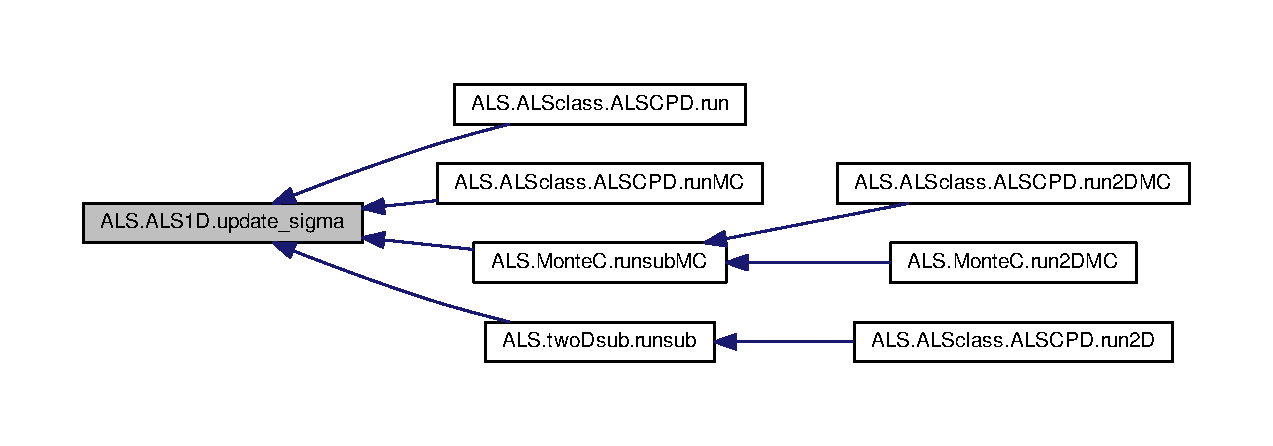
\includegraphics[width=350pt]{namespace_a_l_s_1_1_a_l_s1_d_a994f6e3fde98eeeeb090fd856c2e4844_icgraph}
\end{center}
\end{figure}




\subsection{Variable Documentation}
\hypertarget{namespace_a_l_s_1_1_a_l_s1_d_a6225364b4130ce75f06fc87c2741007f}{\index{A\+L\+S\+::\+A\+L\+S1\+D@{A\+L\+S\+::\+A\+L\+S1\+D}!au2ic@{au2ic}}
\index{au2ic@{au2ic}!A\+L\+S\+::\+A\+L\+S1\+D@{A\+L\+S\+::\+A\+L\+S1\+D}}
\subsubsection[{au2ic}]{\setlength{\rightskip}{0pt plus 5cm}float A\+L\+S.\+A\+L\+S1\+D.\+au2ic = 219474.\+63137}}\label{namespace_a_l_s_1_1_a_l_s1_d_a6225364b4130ce75f06fc87c2741007f}


Definition at line 211 of file A\+L\+S1\+D.\+py.


\hypertarget{namespace_a_l_s_1_1_a_l_s2_d}{\section{A\+L\+S.\+A\+L\+S2\+D Namespace Reference}
\label{namespace_a_l_s_1_1_a_l_s2_d}\index{A\+L\+S.\+A\+L\+S2\+D@{A\+L\+S.\+A\+L\+S2\+D}}
}
\subsection*{Functions}
\begin{DoxyCompactItemize}
\item 
def \hyperlink{namespace_a_l_s_1_1_a_l_s2_d_ae355a657a6cb266847cd420f7adbf562}{assemble\+\_\+\+S2\+D}
\item 
def \hyperlink{namespace_a_l_s_1_1_a_l_s2_d_ad0c2350a690a22c070ed5617dc89b030}{add\+\_\+sigma}
\item 
def \hyperlink{namespace_a_l_s_1_1_a_l_s2_d_a8126baa6025baa3401912c95c6ed49e6}{get\+\_\+b\+\_\+ein2\+D}
\item 
def \hyperlink{namespace_a_l_s_1_1_a_l_s2_d_a634505fa1874ea994674f8d23cd4bdc8}{solve\+\_\+linear2\+D}
\item 
def \hyperlink{namespace_a_l_s_1_1_a_l_s2_d_a3e0c42eb2e5647bdd028eceb6713ca2f}{reconstruct}
\item 
def \hyperlink{namespace_a_l_s_1_1_a_l_s2_d_adab695c6121f997fa80f3ee31c83a0a5}{update2\+D}
\end{DoxyCompactItemize}


\subsection{Function Documentation}
\hypertarget{namespace_a_l_s_1_1_a_l_s2_d_ad0c2350a690a22c070ed5617dc89b030}{\index{A\+L\+S\+::\+A\+L\+S2\+D@{A\+L\+S\+::\+A\+L\+S2\+D}!add\+\_\+sigma@{add\+\_\+sigma}}
\index{add\+\_\+sigma@{add\+\_\+sigma}!A\+L\+S\+::\+A\+L\+S2\+D@{A\+L\+S\+::\+A\+L\+S2\+D}}
\subsubsection[{add\+\_\+sigma}]{\setlength{\rightskip}{0pt plus 5cm}def A\+L\+S.\+A\+L\+S2\+D.\+add\+\_\+sigma (
\begin{DoxyParamCaption}
\item[{}]{S\+\_\+ij, }
\item[{}]{sigma\+\_\+list, }
\item[{}]{j}
\end{DoxyParamCaption}
)}}\label{namespace_a_l_s_1_1_a_l_s2_d_ad0c2350a690a22c070ed5617dc89b030}
\begin{DoxyVerb}Function to implicitly add a sigma of certain index from the complete list to a given two-hole overlap
matrix effectively yielding a one-hole overlap matrix.

[Args]:
        S[array]: Two-hole overlap matrix of shape (r,r).
        sigma_list[list]: List containing the individual terms for the SPP of all DOF.
        j[int]: Index of sigma to be multiplied into the two-hole overlap matrix.
        
[Returns]:
        [array]: One-hole overlap matrix of shape (r,r).\end{DoxyVerb}
 

Definition at line 27 of file A\+L\+S2\+D.\+py.



Here is the caller graph for this function\+:
\nopagebreak
\begin{figure}[H]
\begin{center}
\leavevmode
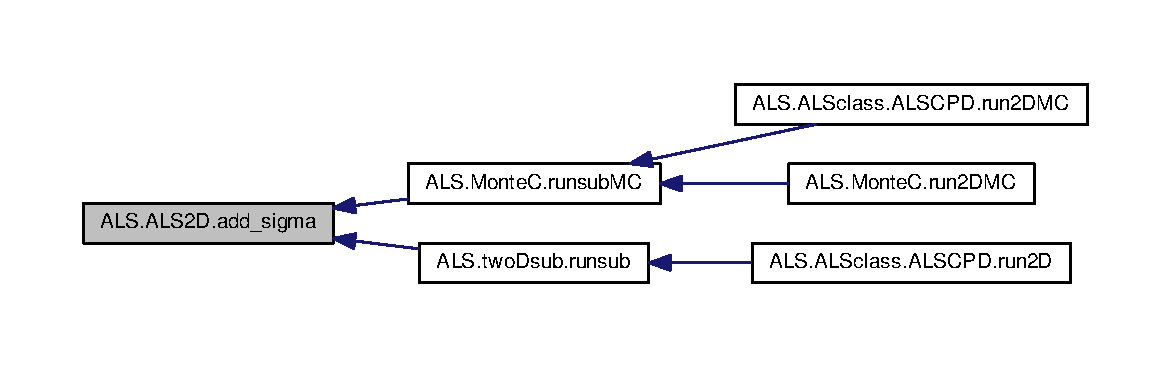
\includegraphics[width=350pt]{namespace_a_l_s_1_1_a_l_s2_d_ad0c2350a690a22c070ed5617dc89b030_icgraph}
\end{center}
\end{figure}


\hypertarget{namespace_a_l_s_1_1_a_l_s2_d_ae355a657a6cb266847cd420f7adbf562}{\index{A\+L\+S\+::\+A\+L\+S2\+D@{A\+L\+S\+::\+A\+L\+S2\+D}!assemble\+\_\+\+S2\+D@{assemble\+\_\+\+S2\+D}}
\index{assemble\+\_\+\+S2\+D@{assemble\+\_\+\+S2\+D}!A\+L\+S\+::\+A\+L\+S2\+D@{A\+L\+S\+::\+A\+L\+S2\+D}}
\subsubsection[{assemble\+\_\+\+S2\+D}]{\setlength{\rightskip}{0pt plus 5cm}def A\+L\+S.\+A\+L\+S2\+D.\+assemble\+\_\+\+S2\+D (
\begin{DoxyParamCaption}
\item[{}]{sigma\+\_\+list, }
\item[{}]{hole1, }
\item[{}]{hole2}
\end{DoxyParamCaption}
)}}\label{namespace_a_l_s_1_1_a_l_s2_d_ae355a657a6cb266847cd420f7adbf562}
\begin{DoxyVerb}Function to assemble the overlap matrix from a given set of sigmas neglecting two sigmas.

[Args]:
        sigma_list[list]: List containing the individual terms for the SPP of all DOF.
        hole1[Int]: Index of the first term to be neglected.
        hole2[Int]: Index of the second term to be neglected.
        
[Returns]:
        [array]: Array containing the two-hole overlap matrix for a given set of SPP.\end{DoxyVerb}
 

Definition at line 8 of file A\+L\+S2\+D.\+py.



Here is the caller graph for this function\+:
\nopagebreak
\begin{figure}[H]
\begin{center}
\leavevmode
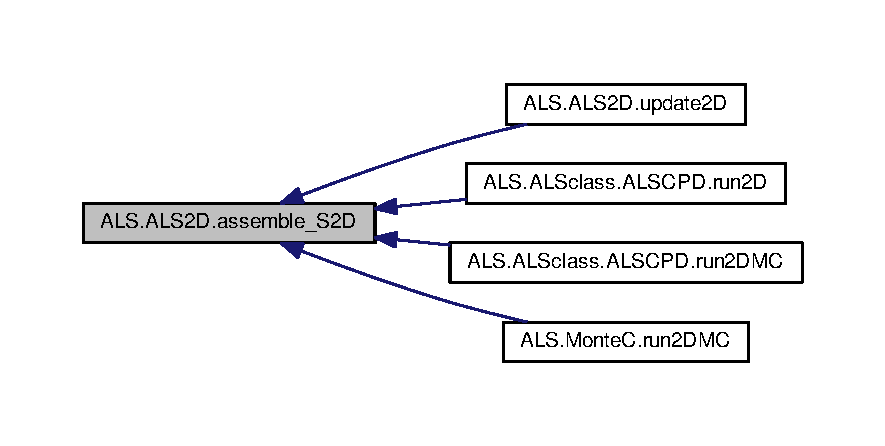
\includegraphics[width=350pt]{namespace_a_l_s_1_1_a_l_s2_d_ae355a657a6cb266847cd420f7adbf562_icgraph}
\end{center}
\end{figure}


\hypertarget{namespace_a_l_s_1_1_a_l_s2_d_a8126baa6025baa3401912c95c6ed49e6}{\index{A\+L\+S\+::\+A\+L\+S2\+D@{A\+L\+S\+::\+A\+L\+S2\+D}!get\+\_\+b\+\_\+ein2\+D@{get\+\_\+b\+\_\+ein2\+D}}
\index{get\+\_\+b\+\_\+ein2\+D@{get\+\_\+b\+\_\+ein2\+D}!A\+L\+S\+::\+A\+L\+S2\+D@{A\+L\+S\+::\+A\+L\+S2\+D}}
\subsubsection[{get\+\_\+b\+\_\+ein2\+D}]{\setlength{\rightskip}{0pt plus 5cm}def A\+L\+S.\+A\+L\+S2\+D.\+get\+\_\+b\+\_\+ein2\+D (
\begin{DoxyParamCaption}
\item[{}]{V, }
\item[{}]{nu\+\_\+r, }
\item[{}]{hole1, }
\item[{}]{hole2}
\end{DoxyParamCaption}
)}}\label{namespace_a_l_s_1_1_a_l_s2_d_a8126baa6025baa3401912c95c6ed49e6}
\begin{DoxyVerb}Function to iteratively create input for the np.einsum routine to contract a given tensor
with given set of SPP for all DOF except two indicated.

[Args]:
        V[array]: The exact tensor to be contracted with shape (N0,N1,N2,...,Nf).
        nu_r[list]: List containing the SPP of all DOF in shape (r,Nk).
        hole1[int]: Index of the first SPP to be neglected.
        hole2[int]: Index of the second SPP to be neglected.
        
[Returns]:
        [Array]: Contracted tensor in shape (r,N[hole1],N[hole2]).
        
-conceptualized and tested assuming hole1 < hole2\end{DoxyVerb}
 

Definition at line 42 of file A\+L\+S2\+D.\+py.



Here is the caller graph for this function\+:
\nopagebreak
\begin{figure}[H]
\begin{center}
\leavevmode
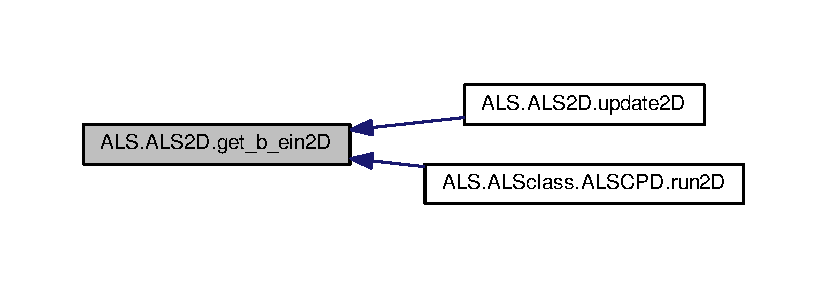
\includegraphics[width=350pt]{namespace_a_l_s_1_1_a_l_s2_d_a8126baa6025baa3401912c95c6ed49e6_icgraph}
\end{center}
\end{figure}


\hypertarget{namespace_a_l_s_1_1_a_l_s2_d_a3e0c42eb2e5647bdd028eceb6713ca2f}{\index{A\+L\+S\+::\+A\+L\+S2\+D@{A\+L\+S\+::\+A\+L\+S2\+D}!reconstruct@{reconstruct}}
\index{reconstruct@{reconstruct}!A\+L\+S\+::\+A\+L\+S2\+D@{A\+L\+S\+::\+A\+L\+S2\+D}}
\subsubsection[{reconstruct}]{\setlength{\rightskip}{0pt plus 5cm}def A\+L\+S.\+A\+L\+S2\+D.\+reconstruct (
\begin{DoxyParamCaption}
\item[{}]{x\+\_\+ij, }
\item[{}]{S\+V\+\_\+error = {\ttfamily None}}
\end{DoxyParamCaption}
)}}\label{namespace_a_l_s_1_1_a_l_s2_d_a3e0c42eb2e5647bdd028eceb6713ca2f}
\begin{DoxyVerb}Function to recover the two SPP and the weights from the solution to the 2D AlS LSE.
It is assumed that only the first singular value and vectors are important for now.

[Args]:
        x_ij[array]: Array of shape (r, Ni, Nj) containing the formal solution to the 2D ALS LSE.
        SV_error[float]: Not used at the moment.
        
[Returns]:
        [array]: (r) shaped array containing the new weights (the first singular value along each r coordinate).
        [array]: (r,Ni) shaped array containing the new normalized SPP for the ith DOF.
        [array]: (r,Nj) shaped array containing the new normalized SPP for the jth DOF.\end{DoxyVerb}
 

Definition at line 173 of file A\+L\+S2\+D.\+py.



Here is the caller graph for this function\+:
\nopagebreak
\begin{figure}[H]
\begin{center}
\leavevmode
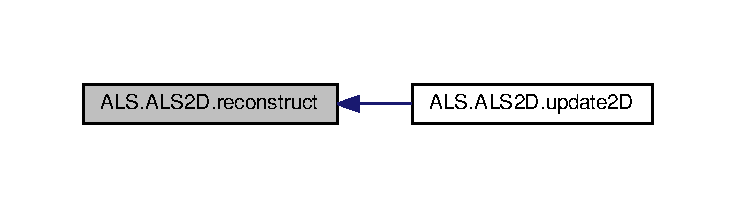
\includegraphics[width=350pt]{namespace_a_l_s_1_1_a_l_s2_d_a3e0c42eb2e5647bdd028eceb6713ca2f_icgraph}
\end{center}
\end{figure}


\hypertarget{namespace_a_l_s_1_1_a_l_s2_d_a634505fa1874ea994674f8d23cd4bdc8}{\index{A\+L\+S\+::\+A\+L\+S2\+D@{A\+L\+S\+::\+A\+L\+S2\+D}!solve\+\_\+linear2\+D@{solve\+\_\+linear2\+D}}
\index{solve\+\_\+linear2\+D@{solve\+\_\+linear2\+D}!A\+L\+S\+::\+A\+L\+S2\+D@{A\+L\+S\+::\+A\+L\+S2\+D}}
\subsubsection[{solve\+\_\+linear2\+D}]{\setlength{\rightskip}{0pt plus 5cm}def A\+L\+S.\+A\+L\+S2\+D.\+solve\+\_\+linear2\+D (
\begin{DoxyParamCaption}
\item[{}]{S\+\_\+ij, }
\item[{}]{b\+\_\+ij, }
\item[{}]{prec = {\ttfamily None}}
\end{DoxyParamCaption}
)}}\label{namespace_a_l_s_1_1_a_l_s2_d_a634505fa1874ea994674f8d23cd4bdc8}
\begin{DoxyVerb}Function to formally solve the linear equation in 2D ALS. The two-hole overlap with the exact tensor
in shape (r, Ni, Nj) is flattened to shape (r, Ni*Nj), the equation is solved and the result
reshaped to(r, Ni, Nj).

[Args]:
        S_ij[array]: Array containing the two-hole overlap matrix of shape (r,r).
        b_ij[array]: Array containing the two-hole overlap with the exact tensor of shape (r, Ni, Nj).
        prec[float]: Gives the epsilon for the regularization, standard is root of machine precision for
                float (~1E-8).
                
[Returns]:
        [array]: Solution of shape (r, Ni, Nj)\end{DoxyVerb}
 

Definition at line 141 of file A\+L\+S2\+D.\+py.



Here is the caller graph for this function\+:
\nopagebreak
\begin{figure}[H]
\begin{center}
\leavevmode
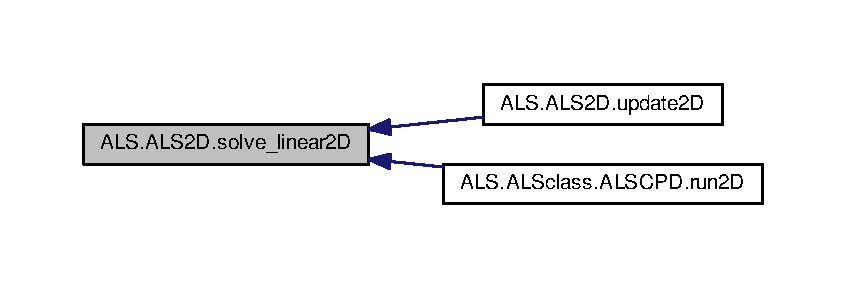
\includegraphics[width=350pt]{namespace_a_l_s_1_1_a_l_s2_d_a634505fa1874ea994674f8d23cd4bdc8_icgraph}
\end{center}
\end{figure}


\hypertarget{namespace_a_l_s_1_1_a_l_s2_d_adab695c6121f997fa80f3ee31c83a0a5}{\index{A\+L\+S\+::\+A\+L\+S2\+D@{A\+L\+S\+::\+A\+L\+S2\+D}!update2\+D@{update2\+D}}
\index{update2\+D@{update2\+D}!A\+L\+S\+::\+A\+L\+S2\+D@{A\+L\+S\+::\+A\+L\+S2\+D}}
\subsubsection[{update2\+D}]{\setlength{\rightskip}{0pt plus 5cm}def A\+L\+S.\+A\+L\+S2\+D.\+update2\+D (
\begin{DoxyParamCaption}
\item[{}]{v\+\_\+ex, }
\item[{}]{nu\+\_\+r, }
\item[{}]{sigmas, }
\item[{}]{i, }
\item[{}]{j, }
\item[{}]{S\+V\+\_\+error = {\ttfamily None}}
\end{DoxyParamCaption}
)}}\label{namespace_a_l_s_1_1_a_l_s2_d_adab695c6121f997fa80f3ee31c83a0a5}
\begin{DoxyVerb}Function to update the weights, the SPP of the ith and the jth DOF.

[Args]:
        v_ex[array]: (N0, N1,...,Nf) shaped array containing the exact tensor.
        nu_r[list]: List containing the SPP for all DOF in shape (r,N).
        sigmas[list]: List containing the sigmas for all DOF in shape (r,r).
        i[int]: First hole index.
        j[int]: Second hole index.
        SV_error[float]: Not used at the moment.
        
[Returns]:
        [array]: (r) shaped array containing the new weights (the first singular value along each r coordinate).
        [array]: (r,Ni) shaped array containing the new normalized SPP for the ith DOF.
        [array]: (r,Nj) shaped array containing the new normalized SPP for the jth DOF.\end{DoxyVerb}
 

Definition at line 211 of file A\+L\+S2\+D.\+py.



Here is the call graph for this function\+:
\nopagebreak
\begin{figure}[H]
\begin{center}
\leavevmode
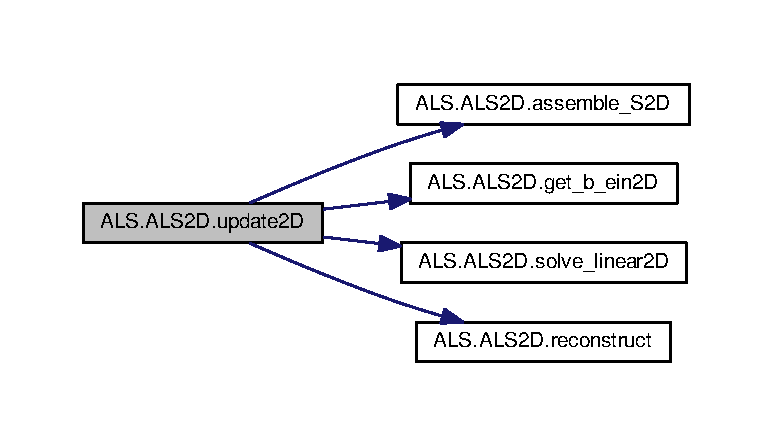
\includegraphics[width=350pt]{namespace_a_l_s_1_1_a_l_s2_d_adab695c6121f997fa80f3ee31c83a0a5_cgraph}
\end{center}
\end{figure}



\hypertarget{namespace_a_l_s_1_1_a_l_sclass}{\section{A\+L\+S.\+A\+L\+Sclass Namespace Reference}
\label{namespace_a_l_s_1_1_a_l_sclass}\index{A\+L\+S.\+A\+L\+Sclass@{A\+L\+S.\+A\+L\+Sclass}}
}
\subsection*{Classes}
\begin{DoxyCompactItemize}
\item 
class \hyperlink{class_a_l_s_1_1_a_l_sclass_1_1_a_l_s_c_p_d}{A\+L\+S\+C\+P\+D}
\end{DoxyCompactItemize}
\subsection*{Variables}
\begin{DoxyCompactItemize}
\item 
float \hyperlink{namespace_a_l_s_1_1_a_l_sclass_a2843ad8c3b497572c7cc5bba0cb32193}{au2ic} = 219474.\+63137
\end{DoxyCompactItemize}


\subsection{Variable Documentation}
\hypertarget{namespace_a_l_s_1_1_a_l_sclass_a2843ad8c3b497572c7cc5bba0cb32193}{\index{A\+L\+S\+::\+A\+L\+Sclass@{A\+L\+S\+::\+A\+L\+Sclass}!au2ic@{au2ic}}
\index{au2ic@{au2ic}!A\+L\+S\+::\+A\+L\+Sclass@{A\+L\+S\+::\+A\+L\+Sclass}}
\subsubsection[{au2ic}]{\setlength{\rightskip}{0pt plus 5cm}float A\+L\+S.\+A\+L\+Sclass.\+au2ic = 219474.\+63137}}\label{namespace_a_l_s_1_1_a_l_sclass_a2843ad8c3b497572c7cc5bba0cb32193}


Definition at line 13 of file A\+L\+Sclass.\+py.


\hypertarget{namespace_a_l_s_1_1dvr}{\section{A\+L\+S.\+dvr Namespace Reference}
\label{namespace_a_l_s_1_1dvr}\index{A\+L\+S.\+dvr@{A\+L\+S.\+dvr}}
}
\subsection*{Classes}
\begin{DoxyCompactItemize}
\item 
class \hyperlink{class_a_l_s_1_1dvr_1_1_d_v_r}{D\+V\+R}
\item 
class \hyperlink{class_a_l_s_1_1dvr_1_1ho_d_v_r}{ho\+D\+V\+R}
\item 
class \hyperlink{class_a_l_s_1_1dvr_1_1sin_d_v_r}{sin\+D\+V\+R}
\end{DoxyCompactItemize}
\subsection*{Functions}
\begin{DoxyCompactItemize}
\item 
def \hyperlink{namespace_a_l_s_1_1dvr_a0710f37ed1119da949db91d6ecf2750c}{sqrt\+\_\+factorial}
\end{DoxyCompactItemize}


\subsection{Function Documentation}
\hypertarget{namespace_a_l_s_1_1dvr_a0710f37ed1119da949db91d6ecf2750c}{\index{A\+L\+S\+::dvr@{A\+L\+S\+::dvr}!sqrt\+\_\+factorial@{sqrt\+\_\+factorial}}
\index{sqrt\+\_\+factorial@{sqrt\+\_\+factorial}!A\+L\+S\+::dvr@{A\+L\+S\+::dvr}}
\subsubsection[{sqrt\+\_\+factorial}]{\setlength{\rightskip}{0pt plus 5cm}def A\+L\+S.\+dvr.\+sqrt\+\_\+factorial (
\begin{DoxyParamCaption}
\item[{}]{n}
\end{DoxyParamCaption}
)}}\label{namespace_a_l_s_1_1dvr_a0710f37ed1119da949db91d6ecf2750c}


Definition at line 21 of file dvr.\+py.


\hypertarget{namespace_a_l_s_1_1h2o}{\section{A\+L\+S.\+h2o Namespace Reference}
\label{namespace_a_l_s_1_1h2o}\index{A\+L\+S.\+h2o@{A\+L\+S.\+h2o}}
}
\subsection*{Functions}
\begin{DoxyCompactItemize}
\item 
def \hyperlink{namespace_a_l_s_1_1h2o_a1723d033fb9b43e41e45e67b84c64a69}{surfh2o}
\item 
def \hyperlink{namespace_a_l_s_1_1h2o_ad076ed0f28a407d6dc919fa686404bd1}{P\+J\+T2\+\_\+2\+D}
\item 
def \hyperlink{namespace_a_l_s_1_1h2o_a43f95d7ca687c002f293a29d43505643}{P\+J\+T2}
\item 
def \hyperlink{namespace_a_l_s_1_1h2o_a148e717fc826a915275d715d7a286472}{vho}
\end{DoxyCompactItemize}


\subsection{Function Documentation}
\hypertarget{namespace_a_l_s_1_1h2o_a43f95d7ca687c002f293a29d43505643}{\index{A\+L\+S\+::h2o@{A\+L\+S\+::h2o}!P\+J\+T2@{P\+J\+T2}}
\index{P\+J\+T2@{P\+J\+T2}!A\+L\+S\+::h2o@{A\+L\+S\+::h2o}}
\subsubsection[{P\+J\+T2}]{\setlength{\rightskip}{0pt plus 5cm}def A\+L\+S.\+h2o.\+P\+J\+T2 (
\begin{DoxyParamCaption}
\item[{}]{Q1, }
\item[{}]{Q2, }
\item[{}]{T\+H\+E\+T\+A}
\end{DoxyParamCaption}
)}}\label{namespace_a_l_s_1_1h2o_a43f95d7ca687c002f293a29d43505643}


Definition at line 46 of file h2o.\+py.



Here is the caller graph for this function\+:
\nopagebreak
\begin{figure}[H]
\begin{center}
\leavevmode
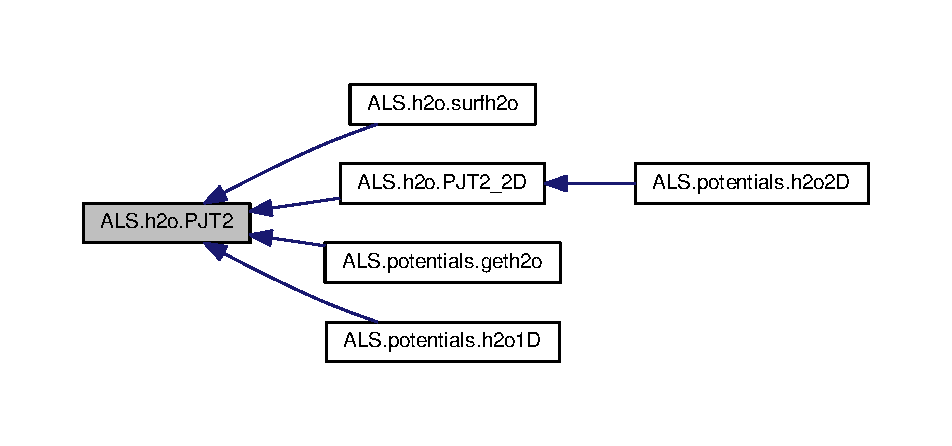
\includegraphics[width=350pt]{namespace_a_l_s_1_1h2o_a43f95d7ca687c002f293a29d43505643_icgraph}
\end{center}
\end{figure}


\hypertarget{namespace_a_l_s_1_1h2o_ad076ed0f28a407d6dc919fa686404bd1}{\index{A\+L\+S\+::h2o@{A\+L\+S\+::h2o}!P\+J\+T2\+\_\+2\+D@{P\+J\+T2\+\_\+2\+D}}
\index{P\+J\+T2\+\_\+2\+D@{P\+J\+T2\+\_\+2\+D}!A\+L\+S\+::h2o@{A\+L\+S\+::h2o}}
\subsubsection[{P\+J\+T2\+\_\+2\+D}]{\setlength{\rightskip}{0pt plus 5cm}def A\+L\+S.\+h2o.\+P\+J\+T2\+\_\+2\+D (
\begin{DoxyParamCaption}
\item[{}]{grd1, }
\item[{}]{grd2, }
\item[{}]{grd3}
\end{DoxyParamCaption}
)}}\label{namespace_a_l_s_1_1h2o_ad076ed0f28a407d6dc919fa686404bd1}


Definition at line 25 of file h2o.\+py.



Here is the call graph for this function\+:
\nopagebreak
\begin{figure}[H]
\begin{center}
\leavevmode
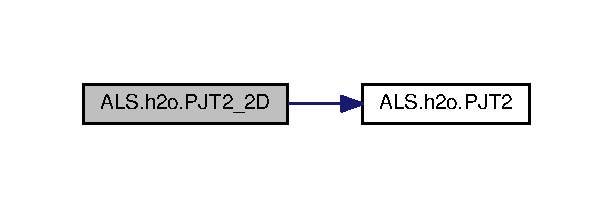
\includegraphics[width=294pt]{namespace_a_l_s_1_1h2o_ad076ed0f28a407d6dc919fa686404bd1_cgraph}
\end{center}
\end{figure}




Here is the caller graph for this function\+:
\nopagebreak
\begin{figure}[H]
\begin{center}
\leavevmode
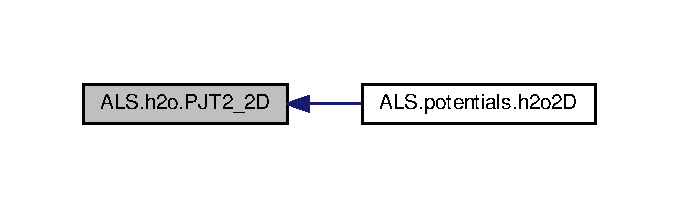
\includegraphics[width=326pt]{namespace_a_l_s_1_1h2o_ad076ed0f28a407d6dc919fa686404bd1_icgraph}
\end{center}
\end{figure}


\hypertarget{namespace_a_l_s_1_1h2o_a1723d033fb9b43e41e45e67b84c64a69}{\index{A\+L\+S\+::h2o@{A\+L\+S\+::h2o}!surfh2o@{surfh2o}}
\index{surfh2o@{surfh2o}!A\+L\+S\+::h2o@{A\+L\+S\+::h2o}}
\subsubsection[{surfh2o}]{\setlength{\rightskip}{0pt plus 5cm}def A\+L\+S.\+h2o.\+surfh2o (
\begin{DoxyParamCaption}
\item[{}]{r1, }
\item[{}]{r4, }
\item[{}]{r2}
\end{DoxyParamCaption}
)}}\label{namespace_a_l_s_1_1h2o_a1723d033fb9b43e41e45e67b84c64a69}


Definition at line 10 of file h2o.\+py.



Here is the call graph for this function\+:
\nopagebreak
\begin{figure}[H]
\begin{center}
\leavevmode
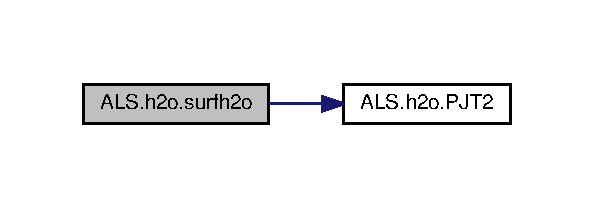
\includegraphics[width=285pt]{namespace_a_l_s_1_1h2o_a1723d033fb9b43e41e45e67b84c64a69_cgraph}
\end{center}
\end{figure}


\hypertarget{namespace_a_l_s_1_1h2o_a148e717fc826a915275d715d7a286472}{\index{A\+L\+S\+::h2o@{A\+L\+S\+::h2o}!vho@{vho}}
\index{vho@{vho}!A\+L\+S\+::h2o@{A\+L\+S\+::h2o}}
\subsubsection[{vho}]{\setlength{\rightskip}{0pt plus 5cm}def A\+L\+S.\+h2o.\+vho (
\begin{DoxyParamCaption}
\item[{}]{r}
\end{DoxyParamCaption}
)}}\label{namespace_a_l_s_1_1h2o_a148e717fc826a915275d715d7a286472}


Definition at line 216 of file h2o.\+py.


\hypertarget{namespace_a_l_s_1_1_monte_c}{\section{A\+L\+S.\+Monte\+C Namespace Reference}
\label{namespace_a_l_s_1_1_monte_c}\index{A\+L\+S.\+Monte\+C@{A\+L\+S.\+Monte\+C}}
}
\subsection*{Functions}
\begin{DoxyCompactItemize}
\item 
def \hyperlink{namespace_a_l_s_1_1_monte_c_af38508f703c31065cca06c8f411e2647}{rndm}
\item 
def \hyperlink{namespace_a_l_s_1_1_monte_c_ad5418939c96212a21f9e3b63306773a3}{get\+\_\+points}
\item 
def \hyperlink{namespace_a_l_s_1_1_monte_c_a3ffcade9d333b987a2a6a5c2aff021fa}{get\+\_\+true\+\_\+points}
\item 
def \hyperlink{namespace_a_l_s_1_1_monte_c_ac7c63eac0a651edb80bc40cf1ac69f5c}{get\+\_\+cut}
\item 
def \hyperlink{namespace_a_l_s_1_1_monte_c_aed6c2eed1b2a9517fc43f90108d43fd6}{get\+\_\+cut2\+D}
\item 
def \hyperlink{namespace_a_l_s_1_1_monte_c_aab81122b0c44d1d6b59570c4b32a0704}{get\+\_\+cuts\+\_\+ind}
\item 
def \hyperlink{namespace_a_l_s_1_1_monte_c_acfabb96f526bf87f1df769e7c32d932d}{get\+\_\+cuts\+\_\+ind2\+D}
\item 
def \hyperlink{namespace_a_l_s_1_1_monte_c_a764b15183b5b4cdfe0e63339822cd37c}{get\+\_\+all\+\_\+cuts}
\item 
def \hyperlink{namespace_a_l_s_1_1_monte_c_a4b3541bda919ddfe1a3f842e7864b0f8}{get\+\_\+all\+\_\+cuts\+\_\+par}
\item 
def \hyperlink{namespace_a_l_s_1_1_monte_c_ac9403f74afc2ad9e4518ab207a185dc3}{get\+\_\+cuts\+\_\+comb\+\_\+par}
\item 
def \hyperlink{namespace_a_l_s_1_1_monte_c_aaee151598865ef3d3847479893261782}{get\+\_\+cuts\+\_\+comb}
\item 
def \hyperlink{namespace_a_l_s_1_1_monte_c_af3153d7f58b8ce542fa113f78bec9495}{get\+\_\+nu\+\_\+smpl}
\item 
def \hyperlink{namespace_a_l_s_1_1_monte_c_a38097cbd2d99540a27cb869d78d8a6ee}{get\+\_\+all\+\_\+nu\+\_\+smpl}
\item 
def \hyperlink{namespace_a_l_s_1_1_monte_c_a91365e6b1de8336973a83bdbcee41cdb}{get\+\_\+omega\+\_\+smpl}
\item 
def \hyperlink{namespace_a_l_s_1_1_monte_c_a68c78d574844f7c4a65605c07a8fd09f}{get\+\_\+omega\+\_\+hole\+\_\+smpl}
\item 
def \hyperlink{namespace_a_l_s_1_1_monte_c_ab12b6535dc175ff87ee5a327d44318b6}{get\+\_\+omega\+\_\+2hole\+\_\+smpl}
\item 
def \hyperlink{namespace_a_l_s_1_1_monte_c_aab6d53ba5a4c94719ab818ad25b7a740}{build\+\_\+d}
\item 
def \hyperlink{namespace_a_l_s_1_1_monte_c_ad12819d80b2961a20bbd0a366aedad70}{build\+\_\+d2d}
\item 
def \hyperlink{namespace_a_l_s_1_1_monte_c_a4358bdd8ce84de8601ec1baa5e079a32}{build\+\_\+\+Z}
\item 
def \hyperlink{namespace_a_l_s_1_1_monte_c_a2be308c6d111eec7697d2d77a5ea516a}{solve\+\_\+linear2\+D\+M\+C}
\item 
def \hyperlink{namespace_a_l_s_1_1_monte_c_afed4abf0b95b57b2c76360c0b8c9f6d5}{update\+\_\+\+M\+C}
\item 
def \hyperlink{namespace_a_l_s_1_1_monte_c_a4b19d241a76bbcad841ce2dca1493a42}{run\+M\+C}
\item 
def \hyperlink{namespace_a_l_s_1_1_monte_c_a3da3c7ee66b0aa86760cd5490341d96d}{runsub\+M\+C}
\item 
def \hyperlink{namespace_a_l_s_1_1_monte_c_a9317dc4284f11d9f8f276424ae6b1a6f}{run2\+D\+M\+C}
\item 
def \hyperlink{namespace_a_l_s_1_1_monte_c_ab73b80288b22e5939d5f107b586a7a44}{setup\+\_\+\+M\+C}
\item 
def \hyperlink{namespace_a_l_s_1_1_monte_c_aec5be61bfee29797502d1274f9a9af2b}{setup\+\_\+\+M\+C2\+D}
\item 
def \hyperlink{namespace_a_l_s_1_1_monte_c_ad7043af53c717e02670f7a93efc0982f}{grab\+\_\+smpl}
\item 
def \hyperlink{namespace_a_l_s_1_1_monte_c_a048b6fcb4b4031bd826f3a4ce2b7e19e}{create\+\_\+comblist}
\end{DoxyCompactItemize}


\subsection{Function Documentation}
\hypertarget{namespace_a_l_s_1_1_monte_c_aab6d53ba5a4c94719ab818ad25b7a740}{\index{A\+L\+S\+::\+Monte\+C@{A\+L\+S\+::\+Monte\+C}!build\+\_\+d@{build\+\_\+d}}
\index{build\+\_\+d@{build\+\_\+d}!A\+L\+S\+::\+Monte\+C@{A\+L\+S\+::\+Monte\+C}}
\subsubsection[{build\+\_\+d}]{\setlength{\rightskip}{0pt plus 5cm}def A\+L\+S.\+Monte\+C.\+build\+\_\+d (
\begin{DoxyParamCaption}
\item[{}]{cut, }
\item[{}]{omega}
\end{DoxyParamCaption}
)}}\label{namespace_a_l_s_1_1_monte_c_aab6d53ba5a4c94719ab818ad25b7a740}
\begin{DoxyVerb}Build the d from the one-hole omega and the corresponding cuts.

[Args]:
        cut[array]: 1D cuts through the potential along one specific coordinate, shape (Ni,s).
        omega[array]: One-hole omega of shape (r,s).
        
[Retuns]:
        [array]: d for the LES of shape (r,Ni).\end{DoxyVerb}
 

Definition at line 356 of file Monte\+C.\+py.



Here is the caller graph for this function\+:
\nopagebreak
\begin{figure}[H]
\begin{center}
\leavevmode
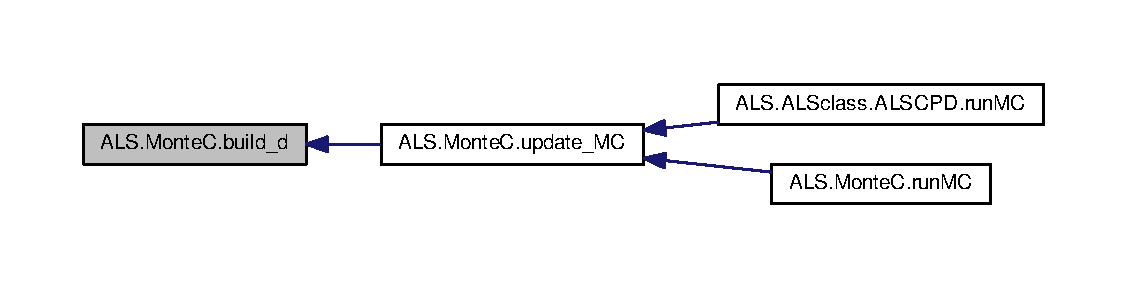
\includegraphics[width=350pt]{namespace_a_l_s_1_1_monte_c_aab6d53ba5a4c94719ab818ad25b7a740_icgraph}
\end{center}
\end{figure}


\hypertarget{namespace_a_l_s_1_1_monte_c_ad12819d80b2961a20bbd0a366aedad70}{\index{A\+L\+S\+::\+Monte\+C@{A\+L\+S\+::\+Monte\+C}!build\+\_\+d2d@{build\+\_\+d2d}}
\index{build\+\_\+d2d@{build\+\_\+d2d}!A\+L\+S\+::\+Monte\+C@{A\+L\+S\+::\+Monte\+C}}
\subsubsection[{build\+\_\+d2d}]{\setlength{\rightskip}{0pt plus 5cm}def A\+L\+S.\+Monte\+C.\+build\+\_\+d2d (
\begin{DoxyParamCaption}
\item[{}]{cuts, }
\item[{}]{omega\+\_\+ij}
\end{DoxyParamCaption}
)}}\label{namespace_a_l_s_1_1_monte_c_ad12819d80b2961a20bbd0a366aedad70}
\begin{DoxyVerb}Build the 2D-d from the two-hole omega and the corresponding cuts.

[Args]:
        cuts[array]: 2D cuts through the potential of shape (Ni,Nk,s).
        omega_ij[array]: Two-hole omega of shape (r,s).
        
[Returns]: 2D-d for the LES of shape (r,Ni,Nk).\end{DoxyVerb}
 

Definition at line 369 of file Monte\+C.\+py.



Here is the caller graph for this function\+:
\nopagebreak
\begin{figure}[H]
\begin{center}
\leavevmode
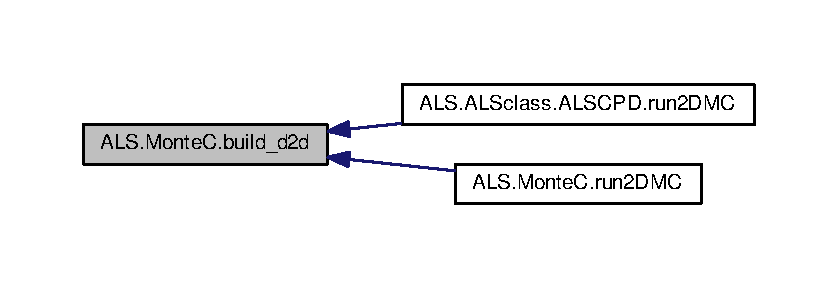
\includegraphics[width=350pt]{namespace_a_l_s_1_1_monte_c_ad12819d80b2961a20bbd0a366aedad70_icgraph}
\end{center}
\end{figure}


\hypertarget{namespace_a_l_s_1_1_monte_c_a4358bdd8ce84de8601ec1baa5e079a32}{\index{A\+L\+S\+::\+Monte\+C@{A\+L\+S\+::\+Monte\+C}!build\+\_\+\+Z@{build\+\_\+\+Z}}
\index{build\+\_\+\+Z@{build\+\_\+\+Z}!A\+L\+S\+::\+Monte\+C@{A\+L\+S\+::\+Monte\+C}}
\subsubsection[{build\+\_\+\+Z}]{\setlength{\rightskip}{0pt plus 5cm}def A\+L\+S.\+Monte\+C.\+build\+\_\+\+Z (
\begin{DoxyParamCaption}
\item[{}]{omega}
\end{DoxyParamCaption}
)}}\label{namespace_a_l_s_1_1_monte_c_a4358bdd8ce84de8601ec1baa5e079a32}
\begin{DoxyVerb}Build the Z from the one-hole omega.

[Args]:
        omega[array]: One-hole omega of shape (r,s).
        
[Returns]:
        [array]: Z for the LES of shape (r,r').\end{DoxyVerb}
 

Definition at line 381 of file Monte\+C.\+py.



Here is the caller graph for this function\+:
\nopagebreak
\begin{figure}[H]
\begin{center}
\leavevmode
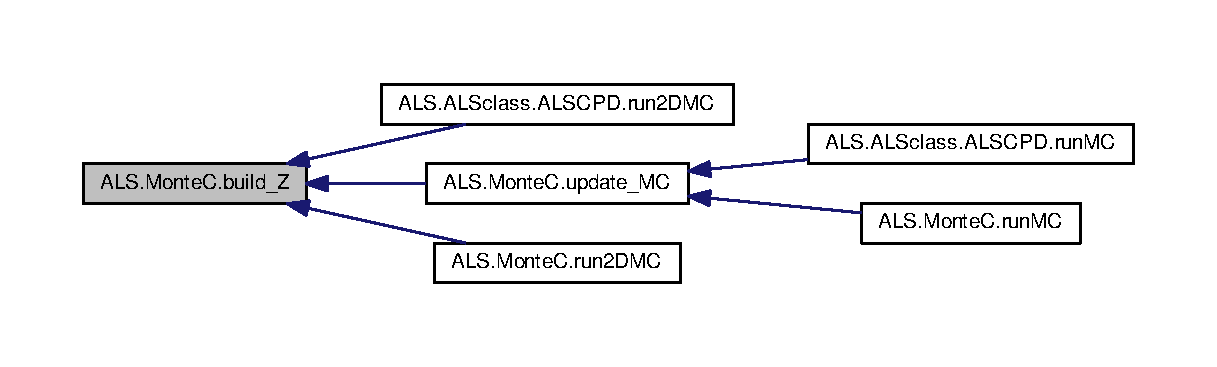
\includegraphics[width=350pt]{namespace_a_l_s_1_1_monte_c_a4358bdd8ce84de8601ec1baa5e079a32_icgraph}
\end{center}
\end{figure}


\hypertarget{namespace_a_l_s_1_1_monte_c_a048b6fcb4b4031bd826f3a4ce2b7e19e}{\index{A\+L\+S\+::\+Monte\+C@{A\+L\+S\+::\+Monte\+C}!create\+\_\+comblist@{create\+\_\+comblist}}
\index{create\+\_\+comblist@{create\+\_\+comblist}!A\+L\+S\+::\+Monte\+C@{A\+L\+S\+::\+Monte\+C}}
\subsubsection[{create\+\_\+comblist}]{\setlength{\rightskip}{0pt plus 5cm}def A\+L\+S.\+Monte\+C.\+create\+\_\+comblist (
\begin{DoxyParamCaption}
\item[{}]{vdim}
\end{DoxyParamCaption}
)}}\label{namespace_a_l_s_1_1_monte_c_a048b6fcb4b4031bd826f3a4ce2b7e19e}
\begin{DoxyVerb}Create the list of all possible and sensible mode combinations.

[Args]:
        vdim[int]: Amount of modes in system.
        
[Returns]:
        [list]: List of lists containing the combinations in index representation.\end{DoxyVerb}
 

Definition at line 689 of file Monte\+C.\+py.



Here is the caller graph for this function\+:
\nopagebreak
\begin{figure}[H]
\begin{center}
\leavevmode
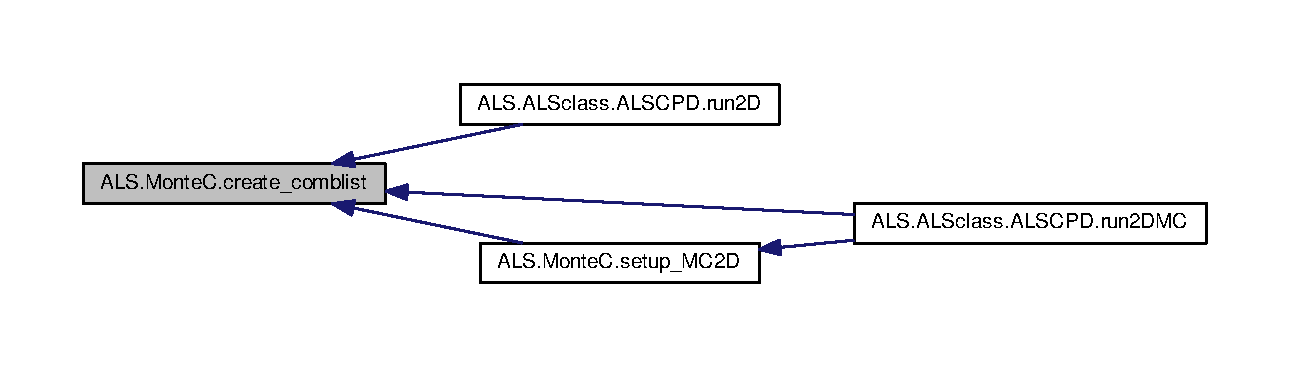
\includegraphics[width=350pt]{namespace_a_l_s_1_1_monte_c_a048b6fcb4b4031bd826f3a4ce2b7e19e_icgraph}
\end{center}
\end{figure}


\hypertarget{namespace_a_l_s_1_1_monte_c_a764b15183b5b4cdfe0e63339822cd37c}{\index{A\+L\+S\+::\+Monte\+C@{A\+L\+S\+::\+Monte\+C}!get\+\_\+all\+\_\+cuts@{get\+\_\+all\+\_\+cuts}}
\index{get\+\_\+all\+\_\+cuts@{get\+\_\+all\+\_\+cuts}!A\+L\+S\+::\+Monte\+C@{A\+L\+S\+::\+Monte\+C}}
\subsubsection[{get\+\_\+all\+\_\+cuts}]{\setlength{\rightskip}{0pt plus 5cm}def A\+L\+S.\+Monte\+C.\+get\+\_\+all\+\_\+cuts (
\begin{DoxyParamCaption}
\item[{}]{constructor, }
\item[{}]{Grid\+\_\+\+List, }
\item[{}]{sample\+\_\+points}
\end{DoxyParamCaption}
)}}\label{namespace_a_l_s_1_1_monte_c_a764b15183b5b4cdfe0e63339822cd37c}
\begin{DoxyVerb}Function to get all cuts along all coordinates for all given sampling points.

[Args]:
        constructor[function]: Function to create the cut from, must be callable with the individual
                    grids along each coordinate.
        Grid_List[list]: List containing the grids for each coordinate used to create the original tensor.
        sample_points[array]: Array of the sampling points of shape (s, np.ndim(V)).
        
[Returns]:
        [list]: List containing the 1D Scans along all of the coordinates for the sampling points
                in shape (Ni,s).\end{DoxyVerb}
 

Definition at line 149 of file Monte\+C.\+py.



Here is the call graph for this function\+:
\nopagebreak
\begin{figure}[H]
\begin{center}
\leavevmode
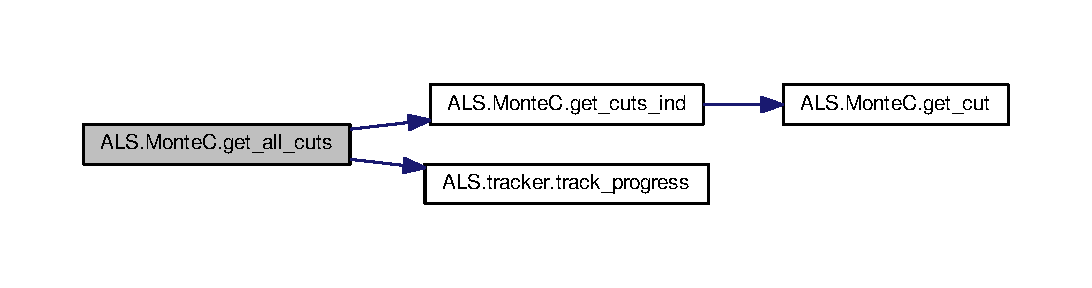
\includegraphics[width=350pt]{namespace_a_l_s_1_1_monte_c_a764b15183b5b4cdfe0e63339822cd37c_cgraph}
\end{center}
\end{figure}


\hypertarget{namespace_a_l_s_1_1_monte_c_a4b3541bda919ddfe1a3f842e7864b0f8}{\index{A\+L\+S\+::\+Monte\+C@{A\+L\+S\+::\+Monte\+C}!get\+\_\+all\+\_\+cuts\+\_\+par@{get\+\_\+all\+\_\+cuts\+\_\+par}}
\index{get\+\_\+all\+\_\+cuts\+\_\+par@{get\+\_\+all\+\_\+cuts\+\_\+par}!A\+L\+S\+::\+Monte\+C@{A\+L\+S\+::\+Monte\+C}}
\subsubsection[{get\+\_\+all\+\_\+cuts\+\_\+par}]{\setlength{\rightskip}{0pt plus 5cm}def A\+L\+S.\+Monte\+C.\+get\+\_\+all\+\_\+cuts\+\_\+par (
\begin{DoxyParamCaption}
\item[{}]{constructor, }
\item[{}]{Grid\+\_\+\+List, }
\item[{}]{sample\+\_\+points}
\end{DoxyParamCaption}
)}}\label{namespace_a_l_s_1_1_monte_c_a4b3541bda919ddfe1a3f842e7864b0f8}


Definition at line 170 of file Monte\+C.\+py.



Here is the call graph for this function\+:
\nopagebreak
\begin{figure}[H]
\begin{center}
\leavevmode
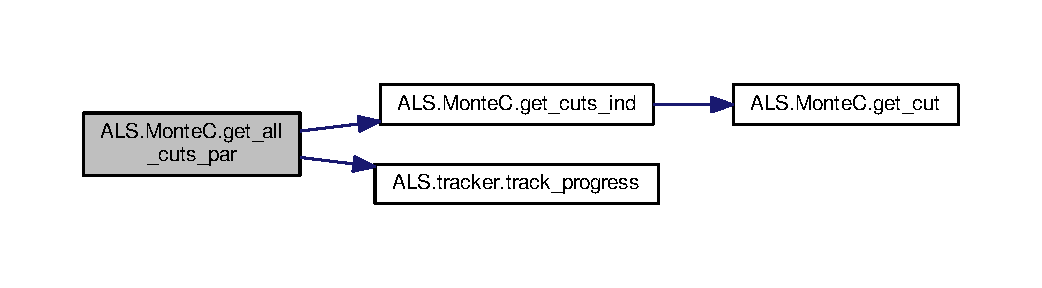
\includegraphics[width=350pt]{namespace_a_l_s_1_1_monte_c_a4b3541bda919ddfe1a3f842e7864b0f8_cgraph}
\end{center}
\end{figure}




Here is the caller graph for this function\+:
\nopagebreak
\begin{figure}[H]
\begin{center}
\leavevmode
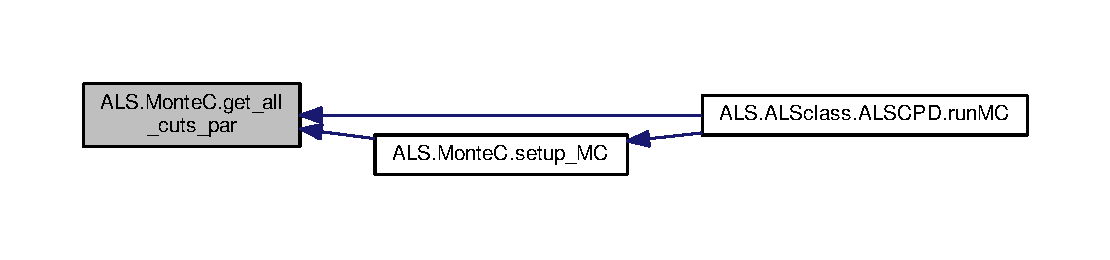
\includegraphics[width=350pt]{namespace_a_l_s_1_1_monte_c_a4b3541bda919ddfe1a3f842e7864b0f8_icgraph}
\end{center}
\end{figure}


\hypertarget{namespace_a_l_s_1_1_monte_c_a38097cbd2d99540a27cb869d78d8a6ee}{\index{A\+L\+S\+::\+Monte\+C@{A\+L\+S\+::\+Monte\+C}!get\+\_\+all\+\_\+nu\+\_\+smpl@{get\+\_\+all\+\_\+nu\+\_\+smpl}}
\index{get\+\_\+all\+\_\+nu\+\_\+smpl@{get\+\_\+all\+\_\+nu\+\_\+smpl}!A\+L\+S\+::\+Monte\+C@{A\+L\+S\+::\+Monte\+C}}
\subsubsection[{get\+\_\+all\+\_\+nu\+\_\+smpl}]{\setlength{\rightskip}{0pt plus 5cm}def A\+L\+S.\+Monte\+C.\+get\+\_\+all\+\_\+nu\+\_\+smpl (
\begin{DoxyParamCaption}
\item[{}]{nu\+\_\+list, }
\item[{}]{smpl\+\_\+idx}
\end{DoxyParamCaption}
)}}\label{namespace_a_l_s_1_1_monte_c_a38097cbd2d99540a27cb869d78d8a6ee}
\begin{DoxyVerb}Function to get the mapped SPP for all DOF.

[Args]:
        nu_list[list]: List containing the SPP in shape (r,N).
        smpl_idx[array]: Array of shape (s,len(nu_list)) containing the sampling points in
                    index representation.
                    
[Returns]:
        [array]: Array containing the new mapped SPP in shape (r,s) along the first axis.\end{DoxyVerb}
 

Definition at line 286 of file Monte\+C.\+py.



Here is the call graph for this function\+:
\nopagebreak
\begin{figure}[H]
\begin{center}
\leavevmode
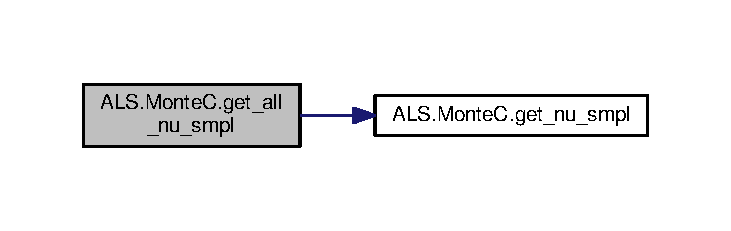
\includegraphics[width=350pt]{namespace_a_l_s_1_1_monte_c_a38097cbd2d99540a27cb869d78d8a6ee_cgraph}
\end{center}
\end{figure}




Here is the caller graph for this function\+:
\nopagebreak
\begin{figure}[H]
\begin{center}
\leavevmode
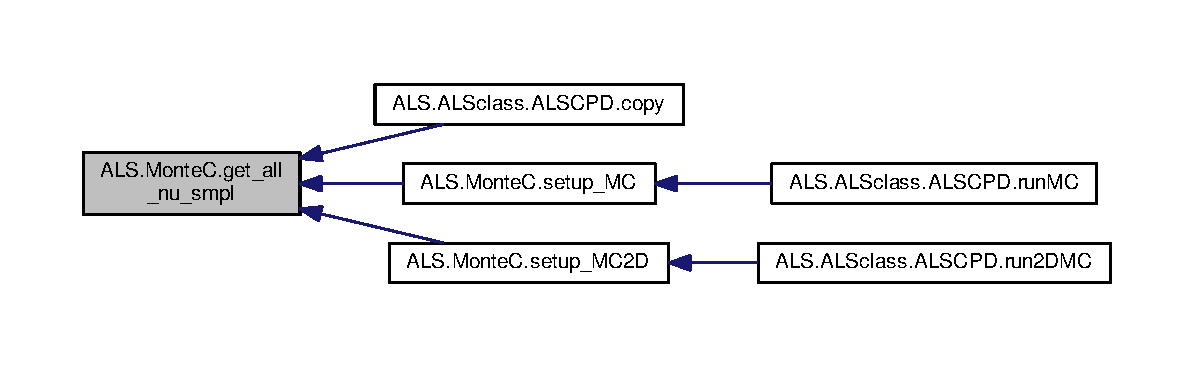
\includegraphics[width=350pt]{namespace_a_l_s_1_1_monte_c_a38097cbd2d99540a27cb869d78d8a6ee_icgraph}
\end{center}
\end{figure}


\hypertarget{namespace_a_l_s_1_1_monte_c_ac7c63eac0a651edb80bc40cf1ac69f5c}{\index{A\+L\+S\+::\+Monte\+C@{A\+L\+S\+::\+Monte\+C}!get\+\_\+cut@{get\+\_\+cut}}
\index{get\+\_\+cut@{get\+\_\+cut}!A\+L\+S\+::\+Monte\+C@{A\+L\+S\+::\+Monte\+C}}
\subsubsection[{get\+\_\+cut}]{\setlength{\rightskip}{0pt plus 5cm}def A\+L\+S.\+Monte\+C.\+get\+\_\+cut (
\begin{DoxyParamCaption}
\item[{}]{constructor, }
\item[{}]{grid, }
\item[{}]{gridindex, }
\item[{}]{sample\+\_\+point}
\end{DoxyParamCaption}
)}}\label{namespace_a_l_s_1_1_monte_c_ac7c63eac0a651edb80bc40cf1ac69f5c}
\begin{DoxyVerb}Function to get a cut through a given function object along one individual grid for a 
given sample point.

[Args]:
        constructor[function]: Function to create the cut from, must be callable by the individual
                    grids along each coordinate.
        grid[array]: Grid along which the cut should be represented. Shape (Ni,)
        gridindex[int]: Index of the grid to cut along.
        sample_point[list]: List of len np.ndim(V) containing the value for each coordinate in this sample point.
        
[Returns]:
        [array]: Cut through the potential of shape (Ni,).\end{DoxyVerb}
 

Definition at line 63 of file Monte\+C.\+py.



Here is the caller graph for this function\+:
\nopagebreak
\begin{figure}[H]
\begin{center}
\leavevmode
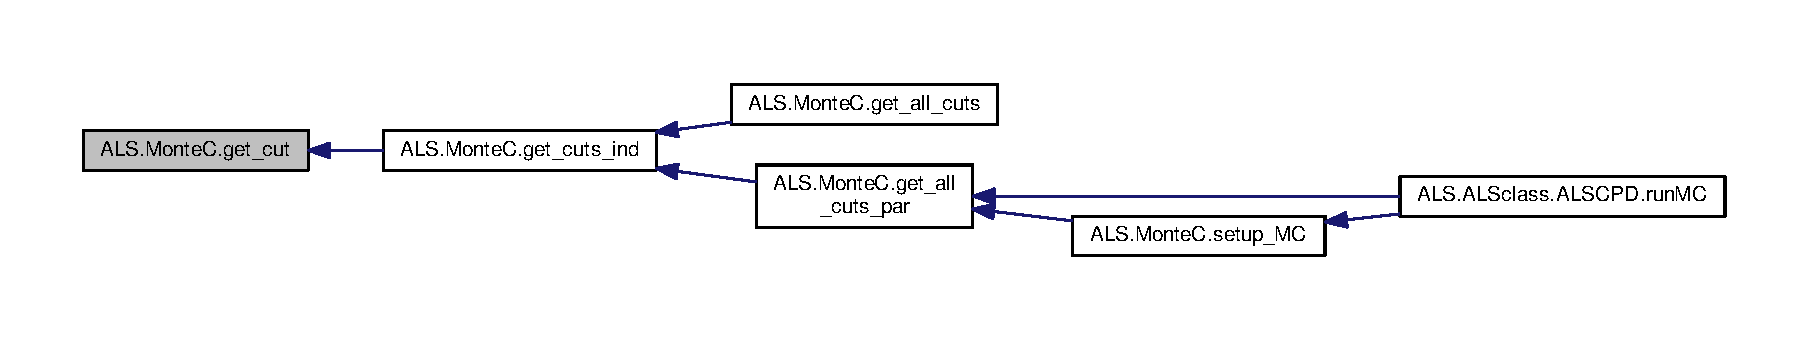
\includegraphics[width=350pt]{namespace_a_l_s_1_1_monte_c_ac7c63eac0a651edb80bc40cf1ac69f5c_icgraph}
\end{center}
\end{figure}


\hypertarget{namespace_a_l_s_1_1_monte_c_aed6c2eed1b2a9517fc43f90108d43fd6}{\index{A\+L\+S\+::\+Monte\+C@{A\+L\+S\+::\+Monte\+C}!get\+\_\+cut2\+D@{get\+\_\+cut2\+D}}
\index{get\+\_\+cut2\+D@{get\+\_\+cut2\+D}!A\+L\+S\+::\+Monte\+C@{A\+L\+S\+::\+Monte\+C}}
\subsubsection[{get\+\_\+cut2\+D}]{\setlength{\rightskip}{0pt plus 5cm}def A\+L\+S.\+Monte\+C.\+get\+\_\+cut2\+D (
\begin{DoxyParamCaption}
\item[{}]{constructor, }
\item[{}]{grd1, }
\item[{}]{grdidx1, }
\item[{}]{grd2, }
\item[{}]{grdidx2, }
\item[{}]{sample\+\_\+point}
\end{DoxyParamCaption}
)}}\label{namespace_a_l_s_1_1_monte_c_aed6c2eed1b2a9517fc43f90108d43fd6}
\begin{DoxyVerb}Function to get a 2D cut through a given function object along two grids for a given sample point.

[Args]:
        constructor[function]: Function to create the cut from, must be callable by the individual
                    grids along each coordinate.
        grd1[array]: Grid for the first coordinate of shape (Ni,).
        grdidx1[int]: Index for the first coordinate.
        grd2[array]: Grid for the second coordinate of shape (Nk,).
        grdidx2[int]: Index for the second coordinate.
        sample_point[array]: Array containing one sample point of shape (np.ndim(V),).

[Returns]:
        [array]: 2D cut along designated coordinates of shape (Ni,Nk)\end{DoxyVerb}
 

Definition at line 86 of file Monte\+C.\+py.



Here is the caller graph for this function\+:
\nopagebreak
\begin{figure}[H]
\begin{center}
\leavevmode
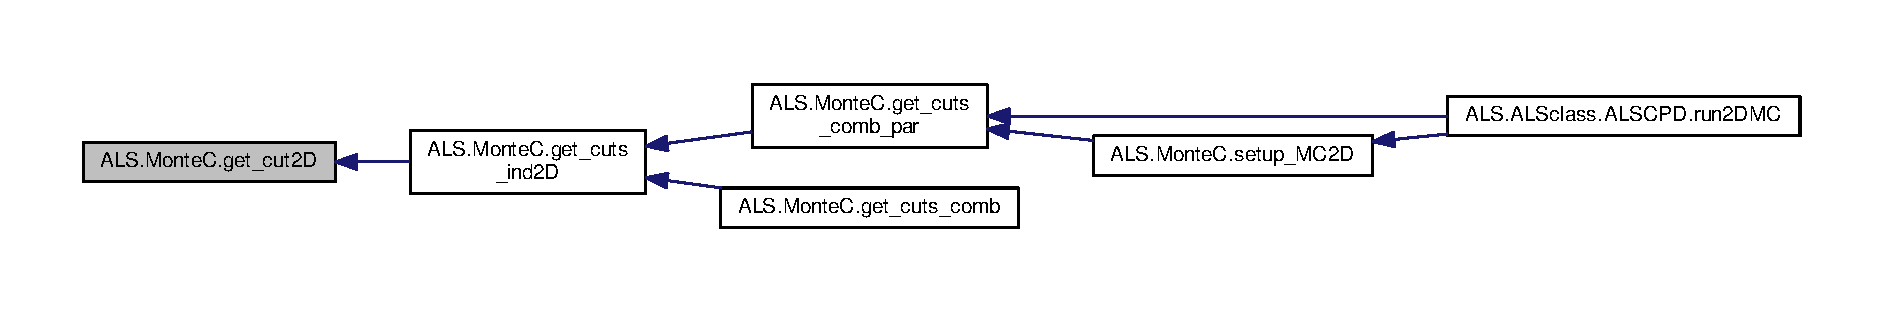
\includegraphics[width=350pt]{namespace_a_l_s_1_1_monte_c_aed6c2eed1b2a9517fc43f90108d43fd6_icgraph}
\end{center}
\end{figure}


\hypertarget{namespace_a_l_s_1_1_monte_c_aaee151598865ef3d3847479893261782}{\index{A\+L\+S\+::\+Monte\+C@{A\+L\+S\+::\+Monte\+C}!get\+\_\+cuts\+\_\+comb@{get\+\_\+cuts\+\_\+comb}}
\index{get\+\_\+cuts\+\_\+comb@{get\+\_\+cuts\+\_\+comb}!A\+L\+S\+::\+Monte\+C@{A\+L\+S\+::\+Monte\+C}}
\subsubsection[{get\+\_\+cuts\+\_\+comb}]{\setlength{\rightskip}{0pt plus 5cm}def A\+L\+S.\+Monte\+C.\+get\+\_\+cuts\+\_\+comb (
\begin{DoxyParamCaption}
\item[{}]{comblist, }
\item[{}]{constructor, }
\item[{}]{Grid\+\_\+\+List, }
\item[{}]{sample\+\_\+points}
\end{DoxyParamCaption}
)}}\label{namespace_a_l_s_1_1_monte_c_aaee151598865ef3d3847479893261782}
\begin{DoxyVerb}Get 2D scans from the potential along the coordinate combinations indicated by the combinations list.

[Args]:
        comblist[list]: List of lists containing the indices for the 2D scans e.g. [[i,j],[i,k]...].
        constructor[function]: Function to create the cut from, must be callable with the individual
                    grids along each coordinate.
        Grid_List[list]: List containing the grids for each coordinate used to create the original tensor.
        sample_points[array]: Array of the sampling points of shape (s, np.ndim(V)).
        
[Returns]:
        [list]: List containing the 2D scans along the indicated coordinate combinations for the sampling
                points in shape (Ni,Nk,s).\end{DoxyVerb}
 

Definition at line 246 of file Monte\+C.\+py.



Here is the call graph for this function\+:
\nopagebreak
\begin{figure}[H]
\begin{center}
\leavevmode
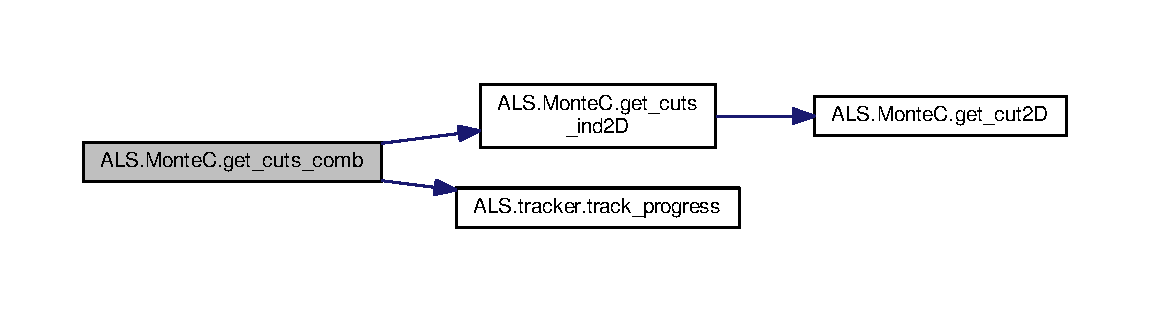
\includegraphics[width=350pt]{namespace_a_l_s_1_1_monte_c_aaee151598865ef3d3847479893261782_cgraph}
\end{center}
\end{figure}


\hypertarget{namespace_a_l_s_1_1_monte_c_ac9403f74afc2ad9e4518ab207a185dc3}{\index{A\+L\+S\+::\+Monte\+C@{A\+L\+S\+::\+Monte\+C}!get\+\_\+cuts\+\_\+comb\+\_\+par@{get\+\_\+cuts\+\_\+comb\+\_\+par}}
\index{get\+\_\+cuts\+\_\+comb\+\_\+par@{get\+\_\+cuts\+\_\+comb\+\_\+par}!A\+L\+S\+::\+Monte\+C@{A\+L\+S\+::\+Monte\+C}}
\subsubsection[{get\+\_\+cuts\+\_\+comb\+\_\+par}]{\setlength{\rightskip}{0pt plus 5cm}def A\+L\+S.\+Monte\+C.\+get\+\_\+cuts\+\_\+comb\+\_\+par (
\begin{DoxyParamCaption}
\item[{}]{comblist, }
\item[{}]{constructor, }
\item[{}]{Grid\+\_\+\+List, }
\item[{}]{sample\+\_\+points}
\end{DoxyParamCaption}
)}}\label{namespace_a_l_s_1_1_monte_c_ac9403f74afc2ad9e4518ab207a185dc3}
\begin{DoxyVerb}Function to parallelize the task of building the 2D cuts. Will try to use as many CPU cores as
it has access to.

[Args]:
        comblist[list]: List containing list with the combinations, e.g. [[i,j],[i,k],...].
        constructor[function]: Function to compute the cuts, should take the grids individually.
        Grid_List[list]: List containing the grids.
        sample_points[array]: Array of the sampling points of shape (s, np.ndim(V)).

[Returns]:
        [list]: List containing the 2D scans along the indicated coordinate combinations for the sampling
                points in shape (Ni,Nk,s).\end{DoxyVerb}
 

Definition at line 197 of file Monte\+C.\+py.



Here is the call graph for this function\+:
\nopagebreak
\begin{figure}[H]
\begin{center}
\leavevmode
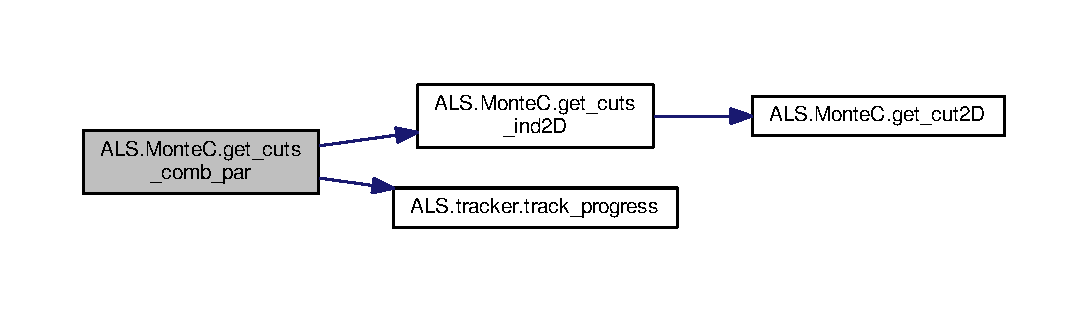
\includegraphics[width=350pt]{namespace_a_l_s_1_1_monte_c_ac9403f74afc2ad9e4518ab207a185dc3_cgraph}
\end{center}
\end{figure}




Here is the caller graph for this function\+:
\nopagebreak
\begin{figure}[H]
\begin{center}
\leavevmode
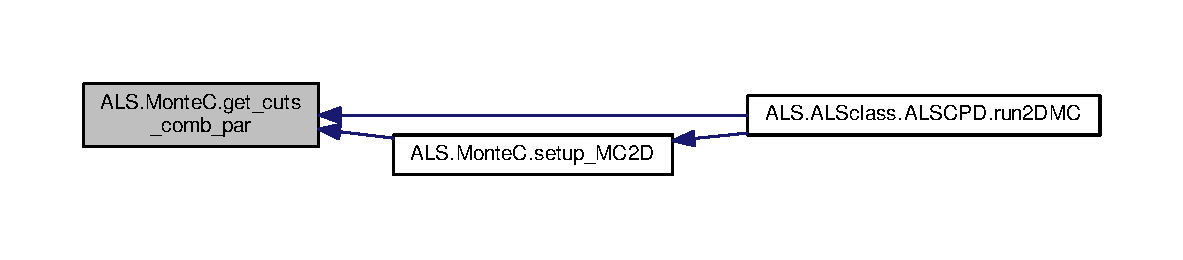
\includegraphics[width=350pt]{namespace_a_l_s_1_1_monte_c_ac9403f74afc2ad9e4518ab207a185dc3_icgraph}
\end{center}
\end{figure}


\hypertarget{namespace_a_l_s_1_1_monte_c_aab81122b0c44d1d6b59570c4b32a0704}{\index{A\+L\+S\+::\+Monte\+C@{A\+L\+S\+::\+Monte\+C}!get\+\_\+cuts\+\_\+ind@{get\+\_\+cuts\+\_\+ind}}
\index{get\+\_\+cuts\+\_\+ind@{get\+\_\+cuts\+\_\+ind}!A\+L\+S\+::\+Monte\+C@{A\+L\+S\+::\+Monte\+C}}
\subsubsection[{get\+\_\+cuts\+\_\+ind}]{\setlength{\rightskip}{0pt plus 5cm}def A\+L\+S.\+Monte\+C.\+get\+\_\+cuts\+\_\+ind (
\begin{DoxyParamCaption}
\item[{}]{constructor, }
\item[{}]{grid, }
\item[{}]{gridindex, }
\item[{}]{sample\+\_\+points}
\end{DoxyParamCaption}
)}}\label{namespace_a_l_s_1_1_monte_c_aab81122b0c44d1d6b59570c4b32a0704}
\begin{DoxyVerb}Function to get all cuts for all sample points for a given coordinate.

[Args]:
        constructor[function]: Function to create the cut from, must be callable with the individual
                    grids along each coordinate.
        grid[array]: Grid along which the cut should be represented. Shape (Ni,)
        gridindex[int]: Index of the grid to cut along.
        sample_points[array]: Array of the sampling points of shape (s, np.ndim(V)).

[Returns]:
        [array]: 1D Scan along coordinate for all sample points, shape (Ni,s).\end{DoxyVerb}
 

Definition at line 108 of file Monte\+C.\+py.



Here is the call graph for this function\+:
\nopagebreak
\begin{figure}[H]
\begin{center}
\leavevmode
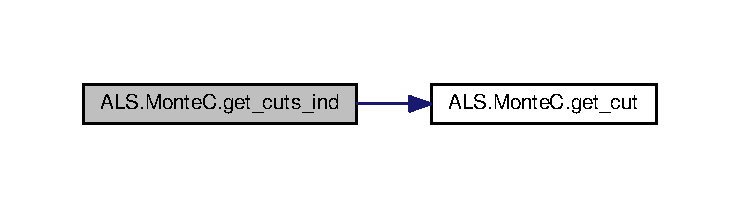
\includegraphics[width=350pt]{namespace_a_l_s_1_1_monte_c_aab81122b0c44d1d6b59570c4b32a0704_cgraph}
\end{center}
\end{figure}




Here is the caller graph for this function\+:
\nopagebreak
\begin{figure}[H]
\begin{center}
\leavevmode
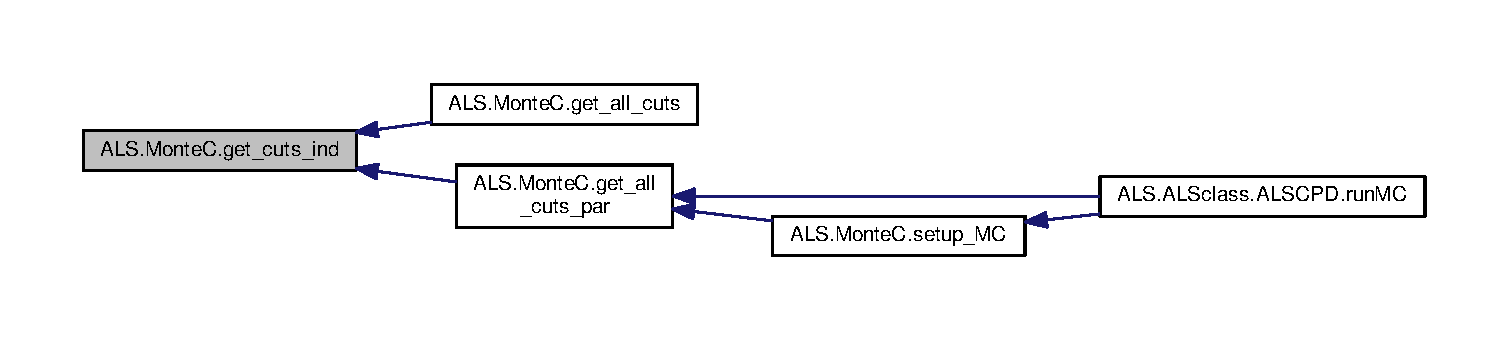
\includegraphics[width=350pt]{namespace_a_l_s_1_1_monte_c_aab81122b0c44d1d6b59570c4b32a0704_icgraph}
\end{center}
\end{figure}


\hypertarget{namespace_a_l_s_1_1_monte_c_acfabb96f526bf87f1df769e7c32d932d}{\index{A\+L\+S\+::\+Monte\+C@{A\+L\+S\+::\+Monte\+C}!get\+\_\+cuts\+\_\+ind2\+D@{get\+\_\+cuts\+\_\+ind2\+D}}
\index{get\+\_\+cuts\+\_\+ind2\+D@{get\+\_\+cuts\+\_\+ind2\+D}!A\+L\+S\+::\+Monte\+C@{A\+L\+S\+::\+Monte\+C}}
\subsubsection[{get\+\_\+cuts\+\_\+ind2\+D}]{\setlength{\rightskip}{0pt plus 5cm}def A\+L\+S.\+Monte\+C.\+get\+\_\+cuts\+\_\+ind2\+D (
\begin{DoxyParamCaption}
\item[{}]{constructor, }
\item[{}]{grd1, }
\item[{}]{grdidx1, }
\item[{}]{grd2, }
\item[{}]{grdidx2, }
\item[{}]{sample\+\_\+points}
\end{DoxyParamCaption}
)}}\label{namespace_a_l_s_1_1_monte_c_acfabb96f526bf87f1df769e7c32d932d}
\begin{DoxyVerb}Function to get all cuts for all sample points for a given combination of coordinates.

[Args]:
        constructor[function]: Function to create the cut from, must be callable with the individual
                    grids along each coordinate.
        grd1[array]: Grid for the first coordinate of shape (Ni,).
        grdidx1[int]: Index for the first coordinate.
        grd2[array]: Grid for the second coordinate of shape (Nk,).
        grdidx2[int]: Index for the second coordinate.
        sample_points[array]: Array containing all sample points in shape (s,np.ndim(V)).
        
[Returns]:
        [array]: 2D scan along coordinates for all sample points, shape (Ni,Nk,s).\end{DoxyVerb}
 

Definition at line 128 of file Monte\+C.\+py.



Here is the call graph for this function\+:
\nopagebreak
\begin{figure}[H]
\begin{center}
\leavevmode
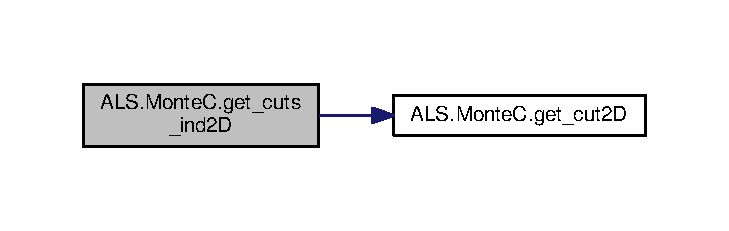
\includegraphics[width=350pt]{namespace_a_l_s_1_1_monte_c_acfabb96f526bf87f1df769e7c32d932d_cgraph}
\end{center}
\end{figure}




Here is the caller graph for this function\+:
\nopagebreak
\begin{figure}[H]
\begin{center}
\leavevmode
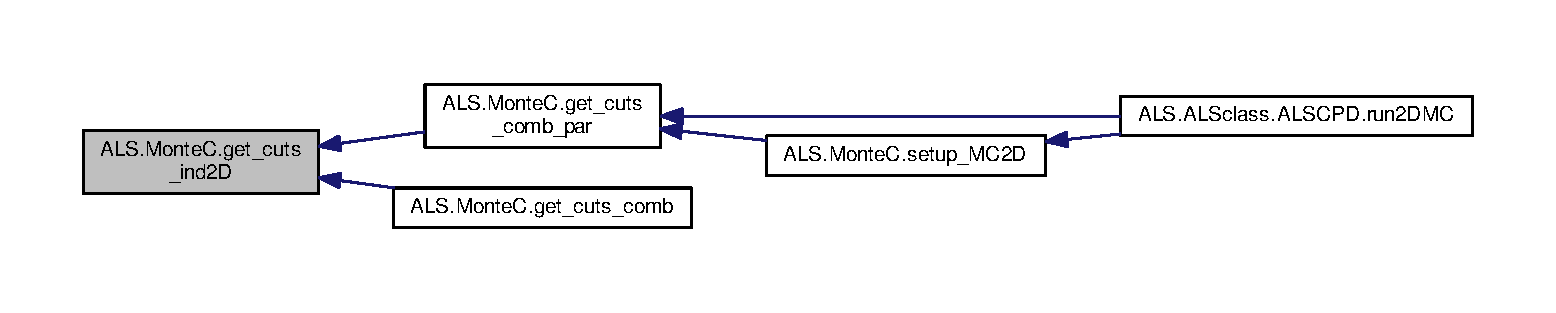
\includegraphics[width=350pt]{namespace_a_l_s_1_1_monte_c_acfabb96f526bf87f1df769e7c32d932d_icgraph}
\end{center}
\end{figure}


\hypertarget{namespace_a_l_s_1_1_monte_c_af3153d7f58b8ce542fa113f78bec9495}{\index{A\+L\+S\+::\+Monte\+C@{A\+L\+S\+::\+Monte\+C}!get\+\_\+nu\+\_\+smpl@{get\+\_\+nu\+\_\+smpl}}
\index{get\+\_\+nu\+\_\+smpl@{get\+\_\+nu\+\_\+smpl}!A\+L\+S\+::\+Monte\+C@{A\+L\+S\+::\+Monte\+C}}
\subsubsection[{get\+\_\+nu\+\_\+smpl}]{\setlength{\rightskip}{0pt plus 5cm}def A\+L\+S.\+Monte\+C.\+get\+\_\+nu\+\_\+smpl (
\begin{DoxyParamCaption}
\item[{}]{nu\+\_\+k, }
\item[{}]{smpl\+\_\+idx\+\_\+k}
\end{DoxyParamCaption}
)}}\label{namespace_a_l_s_1_1_monte_c_af3153d7f58b8ce542fa113f78bec9495}
\begin{DoxyVerb}Function to get one specific sampling SPP by mapping the corresponding sampling
index onto the grid axis of the original SPP.

[Args]:
        nu_k[array]: Original SPP of shape (r, N).
        smpl_idx_k[array]: Array containing the grid indices for the sampling along coordinate.

[Returns]:
        [array]: The mapped SPP from the SPP corresponding to the passed 
                sampling index in shape (r,s).\end{DoxyVerb}
 

Definition at line 268 of file Monte\+C.\+py.



Here is the caller graph for this function\+:
\nopagebreak
\begin{figure}[H]
\begin{center}
\leavevmode
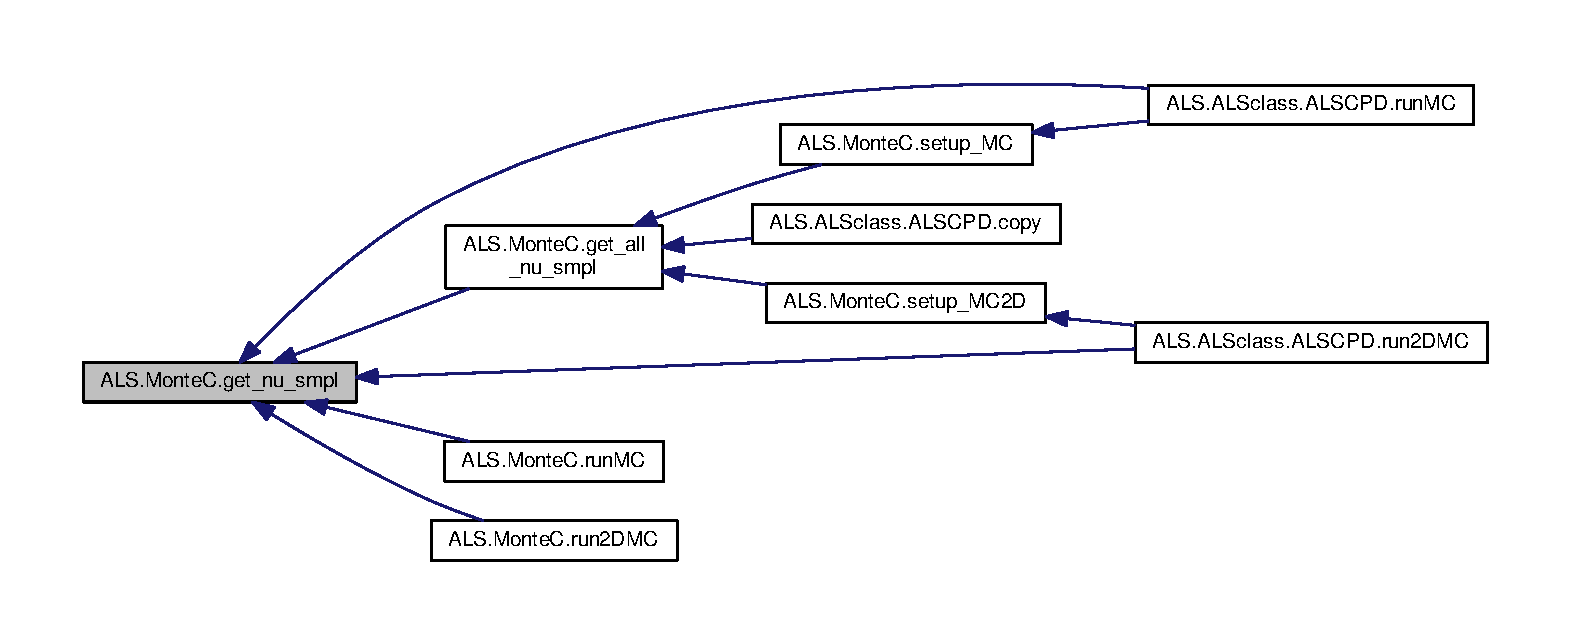
\includegraphics[width=350pt]{namespace_a_l_s_1_1_monte_c_af3153d7f58b8ce542fa113f78bec9495_icgraph}
\end{center}
\end{figure}


\hypertarget{namespace_a_l_s_1_1_monte_c_ab12b6535dc175ff87ee5a327d44318b6}{\index{A\+L\+S\+::\+Monte\+C@{A\+L\+S\+::\+Monte\+C}!get\+\_\+omega\+\_\+2hole\+\_\+smpl@{get\+\_\+omega\+\_\+2hole\+\_\+smpl}}
\index{get\+\_\+omega\+\_\+2hole\+\_\+smpl@{get\+\_\+omega\+\_\+2hole\+\_\+smpl}!A\+L\+S\+::\+Monte\+C@{A\+L\+S\+::\+Monte\+C}}
\subsubsection[{get\+\_\+omega\+\_\+2hole\+\_\+smpl}]{\setlength{\rightskip}{0pt plus 5cm}def A\+L\+S.\+Monte\+C.\+get\+\_\+omega\+\_\+2hole\+\_\+smpl (
\begin{DoxyParamCaption}
\item[{}]{nu\+\_\+smpl, }
\item[{}]{idx1, }
\item[{}]{idx2}
\end{DoxyParamCaption}
)}}\label{namespace_a_l_s_1_1_monte_c_ab12b6535dc175ff87ee5a327d44318b6}
\begin{DoxyVerb}Function to build the two-hole sampled omega by elementwise multiplying the sampled SP
neglecting two indicated.

[Args]:
        nu_smpl[array]: Array containing the sampled SPP in shape (r,s) along the first axis.
        idx1[int]: Index of the first SPP to be neglected.
        idx2[int]: Index of the second SPP to be neglected.
        
[Returns]:
        [array]: Array of shape (r,s) containing the two-hole sampled omega.\end{DoxyVerb}
 

Definition at line 337 of file Monte\+C.\+py.



Here is the caller graph for this function\+:
\nopagebreak
\begin{figure}[H]
\begin{center}
\leavevmode
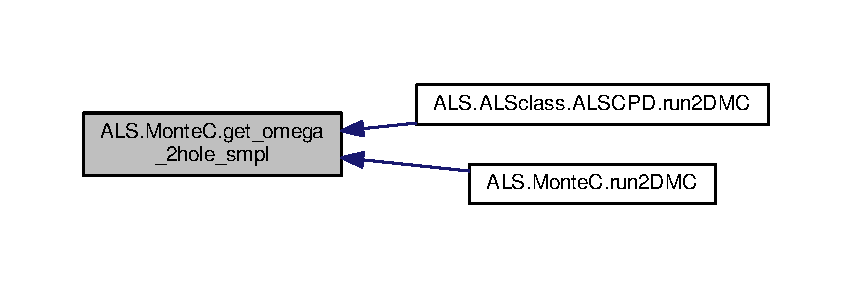
\includegraphics[width=350pt]{namespace_a_l_s_1_1_monte_c_ab12b6535dc175ff87ee5a327d44318b6_icgraph}
\end{center}
\end{figure}


\hypertarget{namespace_a_l_s_1_1_monte_c_a68c78d574844f7c4a65605c07a8fd09f}{\index{A\+L\+S\+::\+Monte\+C@{A\+L\+S\+::\+Monte\+C}!get\+\_\+omega\+\_\+hole\+\_\+smpl@{get\+\_\+omega\+\_\+hole\+\_\+smpl}}
\index{get\+\_\+omega\+\_\+hole\+\_\+smpl@{get\+\_\+omega\+\_\+hole\+\_\+smpl}!A\+L\+S\+::\+Monte\+C@{A\+L\+S\+::\+Monte\+C}}
\subsubsection[{get\+\_\+omega\+\_\+hole\+\_\+smpl}]{\setlength{\rightskip}{0pt plus 5cm}def A\+L\+S.\+Monte\+C.\+get\+\_\+omega\+\_\+hole\+\_\+smpl (
\begin{DoxyParamCaption}
\item[{}]{nu\+\_\+smpl, }
\item[{}]{idx}
\end{DoxyParamCaption}
)}}\label{namespace_a_l_s_1_1_monte_c_a68c78d574844f7c4a65605c07a8fd09f}
\begin{DoxyVerb}Function to build the one-hole sampled omega by elementwise multiplying the sampled SPP
neglecting one indicated.

[Args]:
        nu_smpl[array]: Array containing the sampled SPP in shape (r,s) along the first axis.
        idx[int]: Index of the sampled SPP to be neglected.
       
[Returns]:
        [array]: Array of shape (r,s) containing the one-hole sampled omega.\end{DoxyVerb}
 

Definition at line 318 of file Monte\+C.\+py.



Here is the caller graph for this function\+:
\nopagebreak
\begin{figure}[H]
\begin{center}
\leavevmode
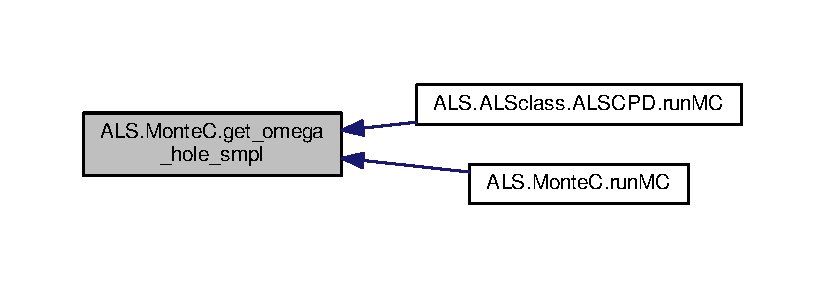
\includegraphics[width=350pt]{namespace_a_l_s_1_1_monte_c_a68c78d574844f7c4a65605c07a8fd09f_icgraph}
\end{center}
\end{figure}


\hypertarget{namespace_a_l_s_1_1_monte_c_a91365e6b1de8336973a83bdbcee41cdb}{\index{A\+L\+S\+::\+Monte\+C@{A\+L\+S\+::\+Monte\+C}!get\+\_\+omega\+\_\+smpl@{get\+\_\+omega\+\_\+smpl}}
\index{get\+\_\+omega\+\_\+smpl@{get\+\_\+omega\+\_\+smpl}!A\+L\+S\+::\+Monte\+C@{A\+L\+S\+::\+Monte\+C}}
\subsubsection[{get\+\_\+omega\+\_\+smpl}]{\setlength{\rightskip}{0pt plus 5cm}def A\+L\+S.\+Monte\+C.\+get\+\_\+omega\+\_\+smpl (
\begin{DoxyParamCaption}
\item[{}]{nu\+\_\+smpl}
\end{DoxyParamCaption}
)}}\label{namespace_a_l_s_1_1_monte_c_a91365e6b1de8336973a83bdbcee41cdb}
\begin{DoxyVerb}Function to build the full sampled omega by elementwise multiplying the sampled SPP.

[Args]:
        nu_smpl[array]: Array containing the sampled SPP in shape (r,s) along the first axis.
       
[Returns]:
        [array]: Array of shape (r,s) containing the full sampled omega.\end{DoxyVerb}
 

Definition at line 302 of file Monte\+C.\+py.

\hypertarget{namespace_a_l_s_1_1_monte_c_ad5418939c96212a21f9e3b63306773a3}{\index{A\+L\+S\+::\+Monte\+C@{A\+L\+S\+::\+Monte\+C}!get\+\_\+points@{get\+\_\+points}}
\index{get\+\_\+points@{get\+\_\+points}!A\+L\+S\+::\+Monte\+C@{A\+L\+S\+::\+Monte\+C}}
\subsubsection[{get\+\_\+points}]{\setlength{\rightskip}{0pt plus 5cm}def A\+L\+S.\+Monte\+C.\+get\+\_\+points (
\begin{DoxyParamCaption}
\item[{}]{Grid\+\_\+\+List, }
\item[{}]{nsmpl}
\end{DoxyParamCaption}
)}}\label{namespace_a_l_s_1_1_monte_c_ad5418939c96212a21f9e3b63306773a3}
\begin{DoxyVerb}Function to get a set amount of sampling points.

[Args]:
        V[array]: The complete tensor.
        nsmpl[int]: Amount of sampling points.
        
[Returns]:
        [array]: Array with the sampling points of shape (s, np.ndim(V)).\end{DoxyVerb}
 

Definition at line 22 of file Monte\+C.\+py.



Here is the call graph for this function\+:
\nopagebreak
\begin{figure}[H]
\begin{center}
\leavevmode
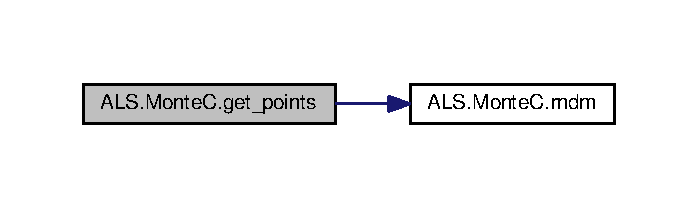
\includegraphics[width=335pt]{namespace_a_l_s_1_1_monte_c_ad5418939c96212a21f9e3b63306773a3_cgraph}
\end{center}
\end{figure}




Here is the caller graph for this function\+:
\nopagebreak
\begin{figure}[H]
\begin{center}
\leavevmode
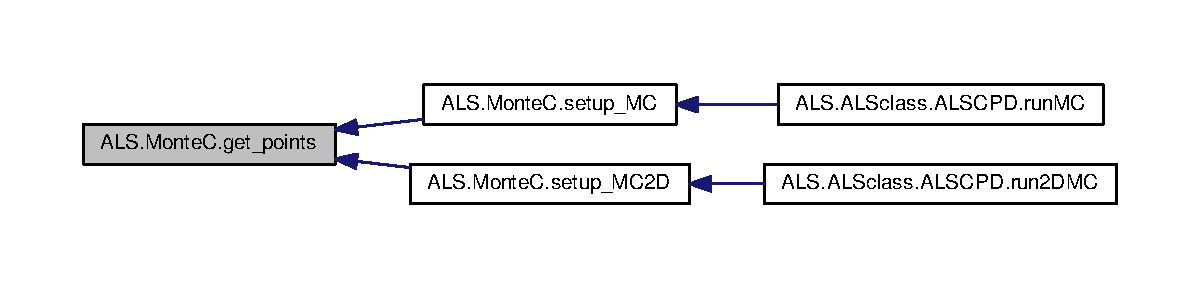
\includegraphics[width=350pt]{namespace_a_l_s_1_1_monte_c_ad5418939c96212a21f9e3b63306773a3_icgraph}
\end{center}
\end{figure}


\hypertarget{namespace_a_l_s_1_1_monte_c_a3ffcade9d333b987a2a6a5c2aff021fa}{\index{A\+L\+S\+::\+Monte\+C@{A\+L\+S\+::\+Monte\+C}!get\+\_\+true\+\_\+points@{get\+\_\+true\+\_\+points}}
\index{get\+\_\+true\+\_\+points@{get\+\_\+true\+\_\+points}!A\+L\+S\+::\+Monte\+C@{A\+L\+S\+::\+Monte\+C}}
\subsubsection[{get\+\_\+true\+\_\+points}]{\setlength{\rightskip}{0pt plus 5cm}def A\+L\+S.\+Monte\+C.\+get\+\_\+true\+\_\+points (
\begin{DoxyParamCaption}
\item[{}]{Grid\+\_\+list, }
\item[{}]{sample\+\_\+points}
\end{DoxyParamCaption}
)}}\label{namespace_a_l_s_1_1_monte_c_a3ffcade9d333b987a2a6a5c2aff021fa}
\begin{DoxyVerb}Function to map the index representation of the sampling points onto the 
corresponding grid points.

[Args]:
        Grid_List[list]: List containing the complete grids for the coordinates.
        sample_points[array]: Array containing the sampling points in index representation.
        
[Returns]:
        [array]: Array containing the sampling points with the corresponding grid coordinates. (s, np.ndim(V))\end{DoxyVerb}
 

Definition at line 40 of file Monte\+C.\+py.



Here is the caller graph for this function\+:
\nopagebreak
\begin{figure}[H]
\begin{center}
\leavevmode
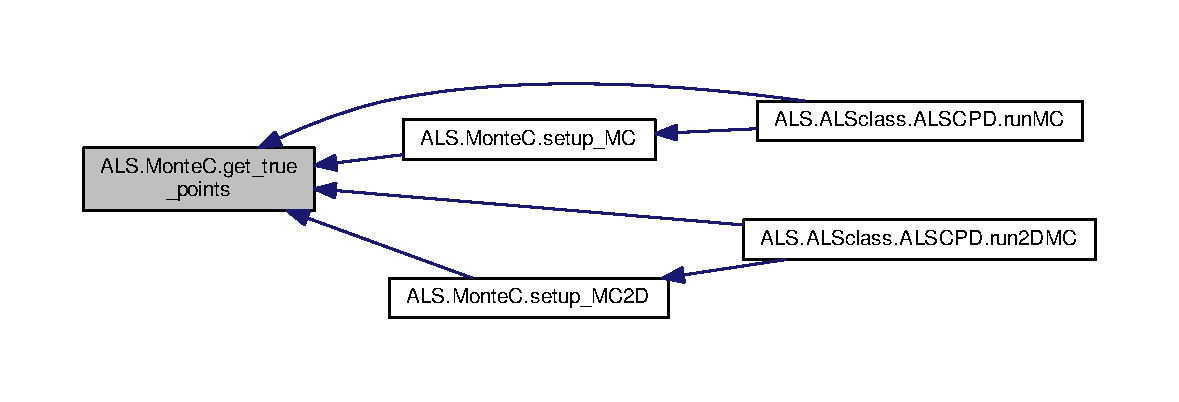
\includegraphics[width=350pt]{namespace_a_l_s_1_1_monte_c_a3ffcade9d333b987a2a6a5c2aff021fa_icgraph}
\end{center}
\end{figure}


\hypertarget{namespace_a_l_s_1_1_monte_c_ad7043af53c717e02670f7a93efc0982f}{\index{A\+L\+S\+::\+Monte\+C@{A\+L\+S\+::\+Monte\+C}!grab\+\_\+smpl@{grab\+\_\+smpl}}
\index{grab\+\_\+smpl@{grab\+\_\+smpl}!A\+L\+S\+::\+Monte\+C@{A\+L\+S\+::\+Monte\+C}}
\subsubsection[{grab\+\_\+smpl}]{\setlength{\rightskip}{0pt plus 5cm}def A\+L\+S.\+Monte\+C.\+grab\+\_\+smpl (
\begin{DoxyParamCaption}
\item[{}]{filename}
\end{DoxyParamCaption}
)}}\label{namespace_a_l_s_1_1_monte_c_ad7043af53c717e02670f7a93efc0982f}
\begin{DoxyVerb}Function to grab presampled points in index representation from a file.

[Args]:
        filename[str]: File to extract the sampling points from. It is assumed that the
                sampling information starts in the second line.
        
[Returns]:
        [array]: Array with the sampling points in shape (s,np.ndim(V)).\end{DoxyVerb}
 

Definition at line 669 of file Monte\+C.\+py.

\hypertarget{namespace_a_l_s_1_1_monte_c_af38508f703c31065cca06c8f411e2647}{\index{A\+L\+S\+::\+Monte\+C@{A\+L\+S\+::\+Monte\+C}!rndm@{rndm}}
\index{rndm@{rndm}!A\+L\+S\+::\+Monte\+C@{A\+L\+S\+::\+Monte\+C}}
\subsubsection[{rndm}]{\setlength{\rightskip}{0pt plus 5cm}def A\+L\+S.\+Monte\+C.\+rndm (
\begin{DoxyParamCaption}
\item[{}]{upper, }
\item[{}]{nsmpl}
\end{DoxyParamCaption}
)}}\label{namespace_a_l_s_1_1_monte_c_af38508f703c31065cca06c8f411e2647}
\begin{DoxyVerb}Function to create a given amount of random integer values in a given half-open interval
with lower border set to 0.

[Args]:
        upper[float]: Upper bound below which values are chosen.
        amount[int]: Number of integer values to return.
        
[Return]:
        [array]: Array containing the random integers.\end{DoxyVerb}
 

Definition at line 8 of file Monte\+C.\+py.



Here is the caller graph for this function\+:
\nopagebreak
\begin{figure}[H]
\begin{center}
\leavevmode
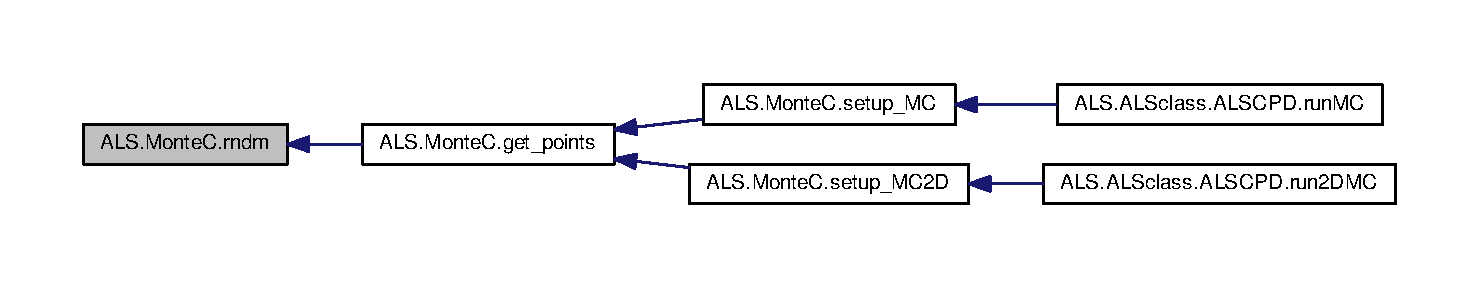
\includegraphics[width=350pt]{namespace_a_l_s_1_1_monte_c_af38508f703c31065cca06c8f411e2647_icgraph}
\end{center}
\end{figure}


\hypertarget{namespace_a_l_s_1_1_monte_c_a9317dc4284f11d9f8f276424ae6b1a6f}{\index{A\+L\+S\+::\+Monte\+C@{A\+L\+S\+::\+Monte\+C}!run2\+D\+M\+C@{run2\+D\+M\+C}}
\index{run2\+D\+M\+C@{run2\+D\+M\+C}!A\+L\+S\+::\+Monte\+C@{A\+L\+S\+::\+Monte\+C}}
\subsubsection[{run2\+D\+M\+C}]{\setlength{\rightskip}{0pt plus 5cm}def A\+L\+S.\+Monte\+C.\+run2\+D\+M\+C (
\begin{DoxyParamCaption}
\item[{}]{V\+\_\+ex, }
\item[{}]{weights, }
\item[{}]{S\+P\+P, }
\item[{}]{nu\+\_\+smpl, }
\item[{}]{comblist, }
\item[{}]{smpl\+\_\+idx, }
\item[{}]{cuts, }
\item[{}]{sigmas, }
\item[{}]{max\+\_\+iter, }
\item[{}]{thresh, }
\item[{}]{prec = {\ttfamily None}}
\end{DoxyParamCaption}
)}}\label{namespace_a_l_s_1_1_monte_c_a9317dc4284f11d9f8f276424ae6b1a6f}
\begin{DoxyVerb}Run the 2DMC-ALSCPD Algorithm.

[Args]:
        V_ex[array]: The exact tensor in shape (Ni,Nj,...,Nf).
        weights[array]: The weights in shape (r,).
        nu_smpl[array]: Array of the sampled SPP in shape (r,s) along first axis.
        comblist[list]: List of list containing the combinations . [[i,j],[i,k]...]
        smpl_idx[array]: Array of the sampling points.
        cuts[list]: List of the 2D cuts for all combinations.
        sigmas[list]: List of the sigmas for the full SPP.
        max_iter[int]: Maximum amount of iterations.
        thresh[float]: Threshhold to signal convergence.
        prec[float]: Value for the regularization, default is ~1E-8.
        
[Returns]:
        [list]: List containing the error for each iteration.\end{DoxyVerb}
 

Definition at line 540 of file Monte\+C.\+py.



Here is the call graph for this function\+:
\nopagebreak
\begin{figure}[H]
\begin{center}
\leavevmode
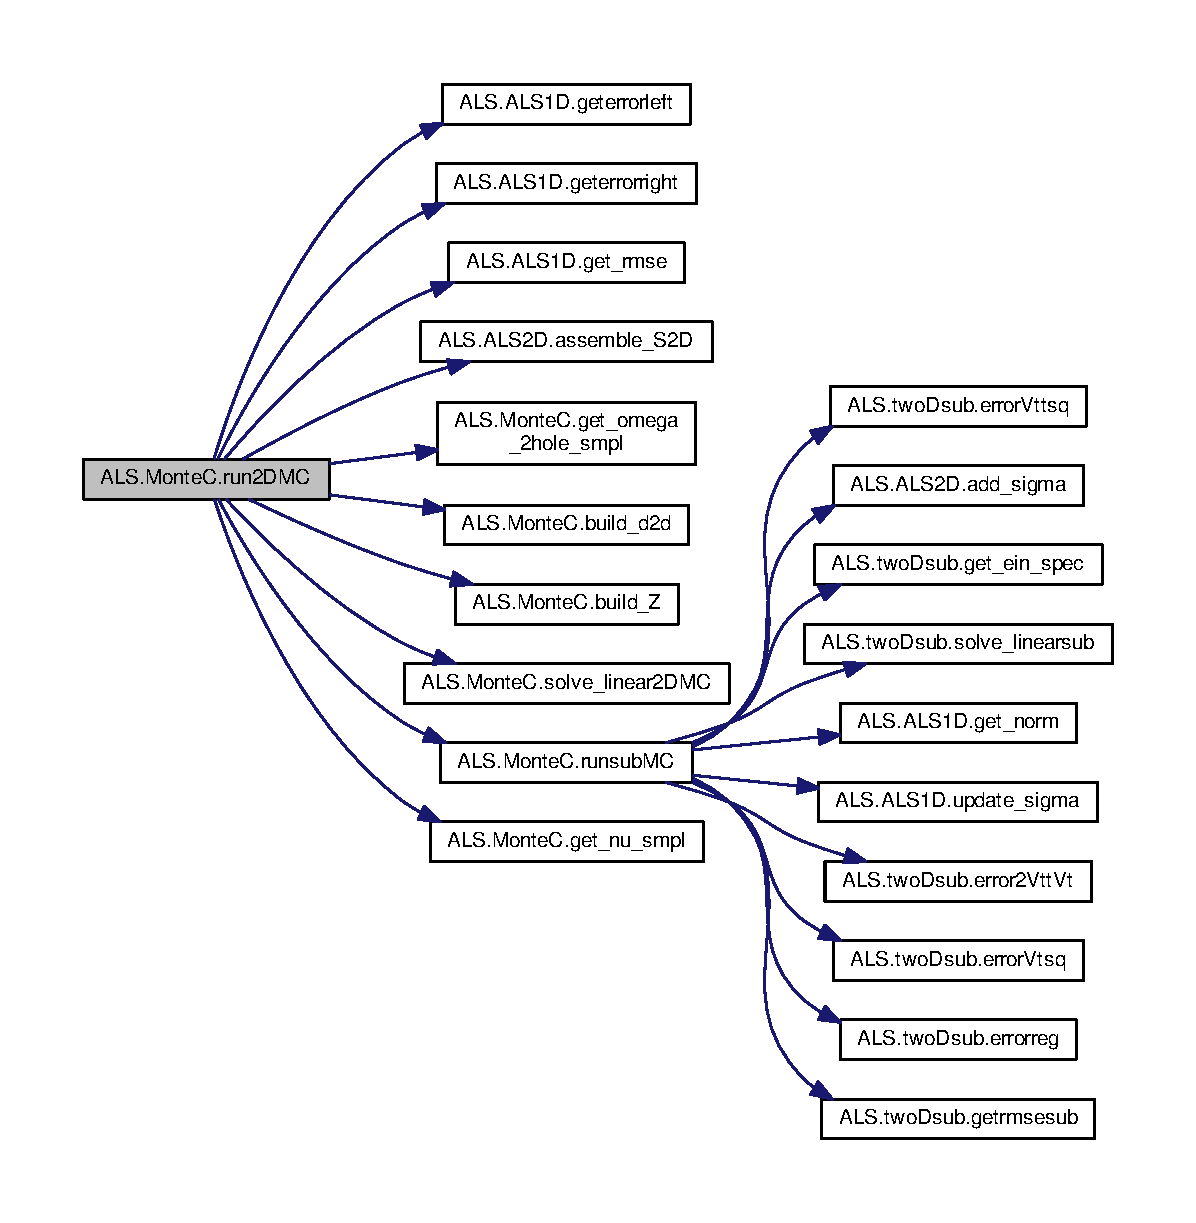
\includegraphics[width=350pt]{namespace_a_l_s_1_1_monte_c_a9317dc4284f11d9f8f276424ae6b1a6f_cgraph}
\end{center}
\end{figure}


\hypertarget{namespace_a_l_s_1_1_monte_c_a4b19d241a76bbcad841ce2dca1493a42}{\index{A\+L\+S\+::\+Monte\+C@{A\+L\+S\+::\+Monte\+C}!run\+M\+C@{run\+M\+C}}
\index{run\+M\+C@{run\+M\+C}!A\+L\+S\+::\+Monte\+C@{A\+L\+S\+::\+Monte\+C}}
\subsubsection[{run\+M\+C}]{\setlength{\rightskip}{0pt plus 5cm}def A\+L\+S.\+Monte\+C.\+run\+M\+C (
\begin{DoxyParamCaption}
\item[{}]{V\+\_\+ex, }
\item[{}]{weights, }
\item[{}]{S\+P\+P, }
\item[{}]{nu\+\_\+smpl, }
\item[{}]{cuts, }
\item[{}]{smpl\+\_\+idx, }
\item[{}]{max\+\_\+iter, }
\item[{}]{thresh}
\end{DoxyParamCaption}
)}}\label{namespace_a_l_s_1_1_monte_c_a4b19d241a76bbcad841ce2dca1493a42}
\begin{DoxyVerb}Function to run the 1D ALSCPD-MC Algorithm.

[Args]:
        V_ex[array]: Exact tensor to compute the error.
        weights[array]: Array of shape (r,) containing the weights.
        SPP[list]: List of the SPP in shape (r,Ni).
        nu_smpl[array]: Array of shape (np.ndim(V),r,s) containing the sampled SPP.
        cuts[list]: List containing the 1D Scans for all DOF.
        smpl_idx[array]: Index representation of the sampling points, shape (s, np.ndim(V)).
        max_iter[int]: Maximum amount of iterations to run.
        thresh[float]: Maximum error to signal convergence.
        
[Returns]:
        [list]: List containing the error for all iterations.\end{DoxyVerb}
 

Definition at line 444 of file Monte\+C.\+py.



Here is the call graph for this function\+:
\nopagebreak
\begin{figure}[H]
\begin{center}
\leavevmode
\includegraphics[width=350pt]{namespace_a_l_s_1_1_monte_c_a4b19d241a76bbcad841ce2dca1493a42_cgraph}
\end{center}
\end{figure}


\hypertarget{namespace_a_l_s_1_1_monte_c_a3da3c7ee66b0aa86760cd5490341d96d}{\index{A\+L\+S\+::\+Monte\+C@{A\+L\+S\+::\+Monte\+C}!runsub\+M\+C@{runsub\+M\+C}}
\index{runsub\+M\+C@{runsub\+M\+C}!A\+L\+S\+::\+Monte\+C@{A\+L\+S\+::\+Monte\+C}}
\subsubsection[{runsub\+M\+C}]{\setlength{\rightskip}{0pt plus 5cm}def A\+L\+S.\+Monte\+C.\+runsub\+M\+C (
\begin{DoxyParamCaption}
\item[{}]{x\+\_\+ij, }
\item[{}]{S\+\_\+ij, }
\item[{}]{weights, }
\item[{}]{S\+P\+P, }
\item[{}]{sigmas, }
\item[{}]{i, }
\item[{}]{j, }
\item[{}]{max\+\_\+it = {\ttfamily 20}, }
\item[{}]{prec = {\ttfamily None}}
\end{DoxyParamCaption}
)}}\label{namespace_a_l_s_1_1_monte_c_a3da3c7ee66b0aa86760cd5490341d96d}
\begin{DoxyVerb}Run the subiterations for the 2DMC-ALS on the full indices.

[Args]:
        x_ij[array]: Solution to the 2DMC LES of shape (r,Ni,Nk).
        S_ij[array]: Two-hole overlap for the full SPP. (r,r).
        weights[array]: Weights of shape (r,).
        SPP[list]: List of the full SPP in shape (r,N).
        sigmas[list]: List of the ovelapmatrices for the SPP of shape (r,r).
        i[int]: Index for the first DOF.
        j[int]: Index for the second DOF.
        max_it[int]: Maximum amount of subiterations, default set to 20.
        prec[float]: Value for the regularization, default is ~1E-8.
        
[Returns]:
        [array]: New weights, shape (r,).
        [list]: Updated list of all SPP in shape (r,N).
        [list]: Updated list of all sigmas in shape (r,r).\end{DoxyVerb}
 

Definition at line 489 of file Monte\+C.\+py.



Here is the call graph for this function\+:
\nopagebreak
\begin{figure}[H]
\begin{center}
\leavevmode
\includegraphics[width=350pt]{namespace_a_l_s_1_1_monte_c_a3da3c7ee66b0aa86760cd5490341d96d_cgraph}
\end{center}
\end{figure}




Here is the caller graph for this function\+:
\nopagebreak
\begin{figure}[H]
\begin{center}
\leavevmode
\includegraphics[width=350pt]{namespace_a_l_s_1_1_monte_c_a3da3c7ee66b0aa86760cd5490341d96d_icgraph}
\end{center}
\end{figure}


\hypertarget{namespace_a_l_s_1_1_monte_c_ab73b80288b22e5939d5f107b586a7a44}{\index{A\+L\+S\+::\+Monte\+C@{A\+L\+S\+::\+Monte\+C}!setup\+\_\+\+M\+C@{setup\+\_\+\+M\+C}}
\index{setup\+\_\+\+M\+C@{setup\+\_\+\+M\+C}!A\+L\+S\+::\+Monte\+C@{A\+L\+S\+::\+Monte\+C}}
\subsubsection[{setup\+\_\+\+M\+C}]{\setlength{\rightskip}{0pt plus 5cm}def A\+L\+S.\+Monte\+C.\+setup\+\_\+\+M\+C (
\begin{DoxyParamCaption}
\item[{}]{grid\+\_\+list, }
\item[{}]{nsmpl, }
\item[{}]{S\+P\+P, }
\item[{}]{constructor}
\end{DoxyParamCaption}
)}}\label{namespace_a_l_s_1_1_monte_c_ab73b80288b22e5939d5f107b586a7a44}
\begin{DoxyVerb}Function to set up the ALSCPD-MC Algorithm.

[Args]:
        grid_list[list]: List containing the original grids for the exact tensor.
        nsmpl[int]: Number of sampling points.
        SPP[list]: List containing the SPP in shape (r,Ni).
        constructor[function]: Function to calculate the potential cuts.
        
[Returns]:
        [array]: Sampling points in index representation of shape (s,np.nidm(V)).
        [list]: List containing the 1D cuts for all DOF in shape (Ni,s).
        [array]: Array of shape (np.ndim(V),r,s) containing the sampled SPP for all DOF.\end{DoxyVerb}
 

Definition at line 615 of file Monte\+C.\+py.



Here is the call graph for this function\+:
\nopagebreak
\begin{figure}[H]
\begin{center}
\leavevmode
\includegraphics[width=350pt]{namespace_a_l_s_1_1_monte_c_ab73b80288b22e5939d5f107b586a7a44_cgraph}
\end{center}
\end{figure}




Here is the caller graph for this function\+:
\nopagebreak
\begin{figure}[H]
\begin{center}
\leavevmode
\includegraphics[width=350pt]{namespace_a_l_s_1_1_monte_c_ab73b80288b22e5939d5f107b586a7a44_icgraph}
\end{center}
\end{figure}


\hypertarget{namespace_a_l_s_1_1_monte_c_aec5be61bfee29797502d1274f9a9af2b}{\index{A\+L\+S\+::\+Monte\+C@{A\+L\+S\+::\+Monte\+C}!setup\+\_\+\+M\+C2\+D@{setup\+\_\+\+M\+C2\+D}}
\index{setup\+\_\+\+M\+C2\+D@{setup\+\_\+\+M\+C2\+D}!A\+L\+S\+::\+Monte\+C@{A\+L\+S\+::\+Monte\+C}}
\subsubsection[{setup\+\_\+\+M\+C2\+D}]{\setlength{\rightskip}{0pt plus 5cm}def A\+L\+S.\+Monte\+C.\+setup\+\_\+\+M\+C2\+D (
\begin{DoxyParamCaption}
\item[{}]{grid\+\_\+list, }
\item[{}]{nsmpl, }
\item[{}]{S\+P\+P, }
\item[{}]{constructor}
\end{DoxyParamCaption}
)}}\label{namespace_a_l_s_1_1_monte_c_aec5be61bfee29797502d1274f9a9af2b}
\begin{DoxyVerb}Function to set up the 2D ALSCPD-MC Algorithm.

[Args]:
        grid_list[list]: List containing the original grids for the exact tensor.
        nsmpl[int]: Number of sampling points.
        SPP[list]: List containing the SPP in shape (r,Ni).
        constructor[function]: Function to calculate the potential cuts.
        
[Returns]:
        [array]: Sampling points in index representation of shape (s,np.nidm(V)).
        [list]: List of lists containing the mode combinations like [[i,j],[i,k],...].
        [list]: List containing the 2D cuts for all DOF in shape (Ni,Nj,s).
        [array]: Array of shape (np.ndim(V),r,s) containing the sampled SPP for all DOF.\end{DoxyVerb}
 

Definition at line 644 of file Monte\+C.\+py.



Here is the call graph for this function\+:
\nopagebreak
\begin{figure}[H]
\begin{center}
\leavevmode
\includegraphics[width=350pt]{namespace_a_l_s_1_1_monte_c_aec5be61bfee29797502d1274f9a9af2b_cgraph}
\end{center}
\end{figure}




Here is the caller graph for this function\+:
\nopagebreak
\begin{figure}[H]
\begin{center}
\leavevmode
\includegraphics[width=350pt]{namespace_a_l_s_1_1_monte_c_aec5be61bfee29797502d1274f9a9af2b_icgraph}
\end{center}
\end{figure}


\hypertarget{namespace_a_l_s_1_1_monte_c_a2be308c6d111eec7697d2d77a5ea516a}{\index{A\+L\+S\+::\+Monte\+C@{A\+L\+S\+::\+Monte\+C}!solve\+\_\+linear2\+D\+M\+C@{solve\+\_\+linear2\+D\+M\+C}}
\index{solve\+\_\+linear2\+D\+M\+C@{solve\+\_\+linear2\+D\+M\+C}!A\+L\+S\+::\+Monte\+C@{A\+L\+S\+::\+Monte\+C}}
\subsubsection[{solve\+\_\+linear2\+D\+M\+C}]{\setlength{\rightskip}{0pt plus 5cm}def A\+L\+S.\+Monte\+C.\+solve\+\_\+linear2\+D\+M\+C (
\begin{DoxyParamCaption}
\item[{}]{Z\+\_\+ij, }
\item[{}]{d\+\_\+ij, }
\item[{}]{prec = {\ttfamily None}}
\end{DoxyParamCaption}
)}}\label{namespace_a_l_s_1_1_monte_c_a2be308c6d111eec7697d2d77a5ea516a}
\begin{DoxyVerb}Solve the LES for the 2DMC Algorithm.

[Args]:
        Z_ij[array]: Two-hole Z of shape (r,r).
        d_ij[array]: Two-hole d of shape (Ni,Nk,s).
        prec[float]: Precision to be used for regularization. Default is sqrt machine prec (~1E-8).
        
[Returns]:
        [array]: Solution to LES of shape (r,Ni,Nk).\end{DoxyVerb}
 

Definition at line 393 of file Monte\+C.\+py.



Here is the caller graph for this function\+:
\nopagebreak
\begin{figure}[H]
\begin{center}
\leavevmode
\includegraphics[width=350pt]{namespace_a_l_s_1_1_monte_c_a2be308c6d111eec7697d2d77a5ea516a_icgraph}
\end{center}
\end{figure}


\hypertarget{namespace_a_l_s_1_1_monte_c_afed4abf0b95b57b2c76360c0b8c9f6d5}{\index{A\+L\+S\+::\+Monte\+C@{A\+L\+S\+::\+Monte\+C}!update\+\_\+\+M\+C@{update\+\_\+\+M\+C}}
\index{update\+\_\+\+M\+C@{update\+\_\+\+M\+C}!A\+L\+S\+::\+Monte\+C@{A\+L\+S\+::\+Monte\+C}}
\subsubsection[{update\+\_\+\+M\+C}]{\setlength{\rightskip}{0pt plus 5cm}def A\+L\+S.\+Monte\+C.\+update\+\_\+\+M\+C (
\begin{DoxyParamCaption}
\item[{}]{nu\+\_\+smpl, }
\item[{}]{omega\+\_\+idx, }
\item[{}]{cut, }
\item[{}]{prec = {\ttfamily None}}
\end{DoxyParamCaption}
)}}\label{namespace_a_l_s_1_1_monte_c_afed4abf0b95b57b2c76360c0b8c9f6d5}
\begin{DoxyVerb}Function to update the SPP for one DOF.

[Args]:
        nu_smpl[array]: Array of shape (np.ndim(V),r,s) containing all sampled SPP.
        omega_idx[array]: One-hole omega of shape (r,s).
        cut[array]: 1D  cuts through the potential along one specific coordinate, shape (Ni,s).
        
[Returns]:
        [array]: Array of shape (r,) containing the new weights.
        [array]: Array of shape (r,Ni) containing the new normalized nu.\end{DoxyVerb}
 

Definition at line 416 of file Monte\+C.\+py.



Here is the call graph for this function\+:
\nopagebreak
\begin{figure}[H]
\begin{center}
\leavevmode
\includegraphics[width=350pt]{namespace_a_l_s_1_1_monte_c_afed4abf0b95b57b2c76360c0b8c9f6d5_cgraph}
\end{center}
\end{figure}




Here is the caller graph for this function\+:
\nopagebreak
\begin{figure}[H]
\begin{center}
\leavevmode
\includegraphics[width=350pt]{namespace_a_l_s_1_1_monte_c_afed4abf0b95b57b2c76360c0b8c9f6d5_icgraph}
\end{center}
\end{figure}



\hypertarget{namespace_a_l_s_1_1potentials}{\section{A\+L\+S.\+potentials Namespace Reference}
\label{namespace_a_l_s_1_1potentials}\index{A\+L\+S.\+potentials@{A\+L\+S.\+potentials}}
}
\subsection*{Functions}
\begin{DoxyCompactItemize}
\item 
def \hyperlink{namespace_a_l_s_1_1potentials_a4a787a8ba107ed1b49a43c2dc5ad8d84}{grab\+\_\+full}
\item 
def \hyperlink{namespace_a_l_s_1_1potentials_a488135d0a6b75e326ef5218aa2d5f95b}{vectorize\+\_\+zundel}
\item 
def \hyperlink{namespace_a_l_s_1_1potentials_a89451020552f9c3a09b5e9f4bab77520}{wrapper\+\_\+zundel}
\item 
def \hyperlink{namespace_a_l_s_1_1potentials_a5f446e677ee72c2d687ec04515df53b4}{geth2o}
\item 
def \hyperlink{namespace_a_l_s_1_1potentials_a11c70ba1da9a8a2c0442d00185c0cd2b}{h2o1\+D}
\item 
def \hyperlink{namespace_a_l_s_1_1potentials_a59a5f031d9eff3ad5a2055055951c1ec}{h2o2\+D}
\item 
def \hyperlink{namespace_a_l_s_1_1potentials_ad7905b747965846c5872695113dd356d}{hfco}
\end{DoxyCompactItemize}


\subsection{Function Documentation}
\hypertarget{namespace_a_l_s_1_1potentials_a5f446e677ee72c2d687ec04515df53b4}{\index{A\+L\+S\+::potentials@{A\+L\+S\+::potentials}!geth2o@{geth2o}}
\index{geth2o@{geth2o}!A\+L\+S\+::potentials@{A\+L\+S\+::potentials}}
\subsubsection[{geth2o}]{\setlength{\rightskip}{0pt plus 5cm}def A\+L\+S.\+potentials.\+geth2o (
\begin{DoxyParamCaption}
\item[{}]{x, }
\item[{}]{y, }
\item[{}]{z}
\end{DoxyParamCaption}
)}}\label{namespace_a_l_s_1_1potentials_a5f446e677ee72c2d687ec04515df53b4}


Definition at line 45 of file potentials.\+py.



Here is the call graph for this function\+:
\nopagebreak
\begin{figure}[H]
\begin{center}
\leavevmode
\includegraphics[width=309pt]{namespace_a_l_s_1_1potentials_a5f446e677ee72c2d687ec04515df53b4_cgraph}
\end{center}
\end{figure}


\hypertarget{namespace_a_l_s_1_1potentials_a4a787a8ba107ed1b49a43c2dc5ad8d84}{\index{A\+L\+S\+::potentials@{A\+L\+S\+::potentials}!grab\+\_\+full@{grab\+\_\+full}}
\index{grab\+\_\+full@{grab\+\_\+full}!A\+L\+S\+::potentials@{A\+L\+S\+::potentials}}
\subsubsection[{grab\+\_\+full}]{\setlength{\rightskip}{0pt plus 5cm}def A\+L\+S.\+potentials.\+grab\+\_\+full (
\begin{DoxyParamCaption}
\item[{}]{filename}
\end{DoxyParamCaption}
)}}\label{namespace_a_l_s_1_1potentials_a4a787a8ba107ed1b49a43c2dc5ad8d84}
\begin{DoxyVerb}Function to load already computed potentials from directory\end{DoxyVerb}
 

Definition at line 6 of file potentials.\+py.



Here is the caller graph for this function\+:
\nopagebreak
\begin{figure}[H]
\begin{center}
\leavevmode
\includegraphics[width=340pt]{namespace_a_l_s_1_1potentials_a4a787a8ba107ed1b49a43c2dc5ad8d84_icgraph}
\end{center}
\end{figure}


\hypertarget{namespace_a_l_s_1_1potentials_a11c70ba1da9a8a2c0442d00185c0cd2b}{\index{A\+L\+S\+::potentials@{A\+L\+S\+::potentials}!h2o1\+D@{h2o1\+D}}
\index{h2o1\+D@{h2o1\+D}!A\+L\+S\+::potentials@{A\+L\+S\+::potentials}}
\subsubsection[{h2o1\+D}]{\setlength{\rightskip}{0pt plus 5cm}def A\+L\+S.\+potentials.\+h2o1\+D (
\begin{DoxyParamCaption}
\item[{}]{x, }
\item[{}]{y, }
\item[{}]{z}
\end{DoxyParamCaption}
)}}\label{namespace_a_l_s_1_1potentials_a11c70ba1da9a8a2c0442d00185c0cd2b}
\begin{DoxyVerb}Call from h2o for 1D.\end{DoxyVerb}
 

Definition at line 49 of file potentials.\+py.



Here is the call graph for this function\+:
\nopagebreak
\begin{figure}[H]
\begin{center}
\leavevmode
\includegraphics[width=308pt]{namespace_a_l_s_1_1potentials_a11c70ba1da9a8a2c0442d00185c0cd2b_cgraph}
\end{center}
\end{figure}


\hypertarget{namespace_a_l_s_1_1potentials_a59a5f031d9eff3ad5a2055055951c1ec}{\index{A\+L\+S\+::potentials@{A\+L\+S\+::potentials}!h2o2\+D@{h2o2\+D}}
\index{h2o2\+D@{h2o2\+D}!A\+L\+S\+::potentials@{A\+L\+S\+::potentials}}
\subsubsection[{h2o2\+D}]{\setlength{\rightskip}{0pt plus 5cm}def A\+L\+S.\+potentials.\+h2o2\+D (
\begin{DoxyParamCaption}
\item[{}]{x, }
\item[{}]{y, }
\item[{}]{z}
\end{DoxyParamCaption}
)}}\label{namespace_a_l_s_1_1potentials_a59a5f031d9eff3ad5a2055055951c1ec}
\begin{DoxyVerb}Call from h2o for 2D.\end{DoxyVerb}
 

Definition at line 53 of file potentials.\+py.



Here is the call graph for this function\+:
\nopagebreak
\begin{figure}[H]
\begin{center}
\leavevmode
\includegraphics[width=350pt]{namespace_a_l_s_1_1potentials_a59a5f031d9eff3ad5a2055055951c1ec_cgraph}
\end{center}
\end{figure}


\hypertarget{namespace_a_l_s_1_1potentials_ad7905b747965846c5872695113dd356d}{\index{A\+L\+S\+::potentials@{A\+L\+S\+::potentials}!hfco@{hfco}}
\index{hfco@{hfco}!A\+L\+S\+::potentials@{A\+L\+S\+::potentials}}
\subsubsection[{hfco}]{\setlength{\rightskip}{0pt plus 5cm}def A\+L\+S.\+potentials.\+hfco (
\begin{DoxyParamCaption}
\item[{}]{x, }
\item[{}]{y, }
\item[{}]{z, }
\item[{}]{w1, }
\item[{}]{w2, }
\item[{}]{w3}
\end{DoxyParamCaption}
)}}\label{namespace_a_l_s_1_1potentials_ad7905b747965846c5872695113dd356d}
\begin{DoxyVerb}Call from hfco.\end{DoxyVerb}
 

Definition at line 57 of file potentials.\+py.

\hypertarget{namespace_a_l_s_1_1potentials_a488135d0a6b75e326ef5218aa2d5f95b}{\index{A\+L\+S\+::potentials@{A\+L\+S\+::potentials}!vectorize\+\_\+zundel@{vectorize\+\_\+zundel}}
\index{vectorize\+\_\+zundel@{vectorize\+\_\+zundel}!A\+L\+S\+::potentials@{A\+L\+S\+::potentials}}
\subsubsection[{vectorize\+\_\+zundel}]{\setlength{\rightskip}{0pt plus 5cm}def A\+L\+S.\+potentials.\+vectorize\+\_\+zundel (
\begin{DoxyParamCaption}
\item[{}]{coordl}
\end{DoxyParamCaption}
)}}\label{namespace_a_l_s_1_1potentials_a488135d0a6b75e326ef5218aa2d5f95b}
\begin{DoxyVerb}function to get cuts through the zundel potential\end{DoxyVerb}
 

Definition at line 11 of file potentials.\+py.



Here is the call graph for this function\+:
\nopagebreak
\begin{figure}[H]
\begin{center}
\leavevmode
\includegraphics[width=350pt]{namespace_a_l_s_1_1potentials_a488135d0a6b75e326ef5218aa2d5f95b_cgraph}
\end{center}
\end{figure}




Here is the caller graph for this function\+:
\nopagebreak
\begin{figure}[H]
\begin{center}
\leavevmode
\includegraphics[width=350pt]{namespace_a_l_s_1_1potentials_a488135d0a6b75e326ef5218aa2d5f95b_icgraph}
\end{center}
\end{figure}


\hypertarget{namespace_a_l_s_1_1potentials_a89451020552f9c3a09b5e9f4bab77520}{\index{A\+L\+S\+::potentials@{A\+L\+S\+::potentials}!wrapper\+\_\+zundel@{wrapper\+\_\+zundel}}
\index{wrapper\+\_\+zundel@{wrapper\+\_\+zundel}!A\+L\+S\+::potentials@{A\+L\+S\+::potentials}}
\subsubsection[{wrapper\+\_\+zundel}]{\setlength{\rightskip}{0pt plus 5cm}def A\+L\+S.\+potentials.\+wrapper\+\_\+zundel (
\begin{DoxyParamCaption}
\item[{}]{grid1, }
\item[{}]{grid2, }
\item[{}]{grid3, }
\item[{}]{grid4, }
\item[{}]{grid5, }
\item[{}]{grid6, }
\item[{}]{grid7, }
\item[{}]{grid8, }
\item[{}]{grid9, }
\item[{}]{grid10, }
\item[{}]{grid11, }
\item[{}]{grid12, }
\item[{}]{grid13, }
\item[{}]{grid14, }
\item[{}]{grid15}
\end{DoxyParamCaption}
)}}\label{namespace_a_l_s_1_1potentials_a89451020552f9c3a09b5e9f4bab77520}
\begin{DoxyVerb}wrapper for the above routine\end{DoxyVerb}
 

Definition at line 39 of file potentials.\+py.



Here is the call graph for this function\+:
\nopagebreak
\begin{figure}[H]
\begin{center}
\leavevmode
\includegraphics[width=350pt]{namespace_a_l_s_1_1potentials_a89451020552f9c3a09b5e9f4bab77520_cgraph}
\end{center}
\end{figure}




Here is the caller graph for this function\+:
\nopagebreak
\begin{figure}[H]
\begin{center}
\leavevmode
\includegraphics[width=350pt]{namespace_a_l_s_1_1potentials_a89451020552f9c3a09b5e9f4bab77520_icgraph}
\end{center}
\end{figure}



\hypertarget{namespace_a_l_s_1_1tracker}{\section{A\+L\+S.\+tracker Namespace Reference}
\label{namespace_a_l_s_1_1tracker}\index{A\+L\+S.\+tracker@{A\+L\+S.\+tracker}}
}
\subsection*{Functions}
\begin{DoxyCompactItemize}
\item 
def \hyperlink{namespace_a_l_s_1_1tracker_afc9db72d13feacd03e5ea9290255c941}{track\+\_\+progress}
\item 
def \hyperlink{namespace_a_l_s_1_1tracker_aacc5f4aca2370c0fd5af2356f66f4eb3}{init\+\_\+tracker}
\item 
def \hyperlink{namespace_a_l_s_1_1tracker_a4d2fa044493765c4db1b95a0769c12df}{keep\+\_\+track}
\end{DoxyCompactItemize}


\subsection{Function Documentation}
\hypertarget{namespace_a_l_s_1_1tracker_aacc5f4aca2370c0fd5af2356f66f4eb3}{\index{A\+L\+S\+::tracker@{A\+L\+S\+::tracker}!init\+\_\+tracker@{init\+\_\+tracker}}
\index{init\+\_\+tracker@{init\+\_\+tracker}!A\+L\+S\+::tracker@{A\+L\+S\+::tracker}}
\subsubsection[{init\+\_\+tracker}]{\setlength{\rightskip}{0pt plus 5cm}def A\+L\+S.\+tracker.\+init\+\_\+tracker (
\begin{DoxyParamCaption}
\item[{}]{max\+\_\+iter}
\end{DoxyParamCaption}
)}}\label{namespace_a_l_s_1_1tracker_aacc5f4aca2370c0fd5af2356f66f4eb3}
\begin{DoxyVerb}Function to initialize the tracker for the ALSCPD class run-Routines.

[Args]:
        max_iter[int]: Maximum amount of iterations possible.
        
[Returns]:
        [array]: Array of length 100 containing the iteration value for each percent of progress.
        [float]: Value between 0 and 1 representing the current progress.
        [int]: Counter keeping track of the currently relevant element from the array above.
        [int]: Curently relevant element from the array above.\end{DoxyVerb}
 

Definition at line 24 of file tracker.\+py.



Here is the caller graph for this function\+:
\nopagebreak
\begin{figure}[H]
\begin{center}
\leavevmode
\includegraphics[width=350pt]{namespace_a_l_s_1_1tracker_aacc5f4aca2370c0fd5af2356f66f4eb3_icgraph}
\end{center}
\end{figure}


\hypertarget{namespace_a_l_s_1_1tracker_a4d2fa044493765c4db1b95a0769c12df}{\index{A\+L\+S\+::tracker@{A\+L\+S\+::tracker}!keep\+\_\+track@{keep\+\_\+track}}
\index{keep\+\_\+track@{keep\+\_\+track}!A\+L\+S\+::tracker@{A\+L\+S\+::tracker}}
\subsubsection[{keep\+\_\+track}]{\setlength{\rightskip}{0pt plus 5cm}def A\+L\+S.\+tracker.\+keep\+\_\+track (
\begin{DoxyParamCaption}
\item[{}]{task, }
\item[{}]{error, }
\item[{}]{perc\+\_\+iter, }
\item[{}]{perc\+\_\+cur, }
\item[{}]{track, }
\item[{}]{cur\+\_\+perc}
\end{DoxyParamCaption}
)}}\label{namespace_a_l_s_1_1tracker_a4d2fa044493765c4db1b95a0769c12df}
\begin{DoxyVerb}Function to update the tracker for the ALSCPD class run-Routines.\end{DoxyVerb}
 

Definition at line 44 of file tracker.\+py.



Here is the call graph for this function\+:
\nopagebreak
\begin{figure}[H]
\begin{center}
\leavevmode
\includegraphics[width=350pt]{namespace_a_l_s_1_1tracker_a4d2fa044493765c4db1b95a0769c12df_cgraph}
\end{center}
\end{figure}




Here is the caller graph for this function\+:
\nopagebreak
\begin{figure}[H]
\begin{center}
\leavevmode
\includegraphics[width=350pt]{namespace_a_l_s_1_1tracker_a4d2fa044493765c4db1b95a0769c12df_icgraph}
\end{center}
\end{figure}


\hypertarget{namespace_a_l_s_1_1tracker_afc9db72d13feacd03e5ea9290255c941}{\index{A\+L\+S\+::tracker@{A\+L\+S\+::tracker}!track\+\_\+progress@{track\+\_\+progress}}
\index{track\+\_\+progress@{track\+\_\+progress}!A\+L\+S\+::tracker@{A\+L\+S\+::tracker}}
\subsubsection[{track\+\_\+progress}]{\setlength{\rightskip}{0pt plus 5cm}def A\+L\+S.\+tracker.\+track\+\_\+progress (
\begin{DoxyParamCaption}
\item[{}]{task, }
\item[{}]{progress, }
\item[{}]{status = {\ttfamily ''}}
\end{DoxyParamCaption}
)}}\label{namespace_a_l_s_1_1tracker_afc9db72d13feacd03e5ea9290255c941}
\begin{DoxyVerb}Function to display the progress of a task.

[Args]:
        task[str]: What task is beeing tracked.
        progress[float]: Value between 0 and 1.
        status[str]: Status to be printed.\end{DoxyVerb}
 

Definition at line 3 of file tracker.\+py.



Here is the caller graph for this function\+:
\nopagebreak
\begin{figure}[H]
\begin{center}
\leavevmode
\includegraphics[width=350pt]{namespace_a_l_s_1_1tracker_afc9db72d13feacd03e5ea9290255c941_icgraph}
\end{center}
\end{figure}



\hypertarget{namespace_a_l_s_1_1two_dsub}{\section{A\+L\+S.\+two\+Dsub Namespace Reference}
\label{namespace_a_l_s_1_1two_dsub}\index{A\+L\+S.\+two\+Dsub@{A\+L\+S.\+two\+Dsub}}
}
\subsection*{Functions}
\begin{DoxyCompactItemize}
\item 
def \hyperlink{namespace_a_l_s_1_1two_dsub_a2f5605fed0568b72d992d8e6cea524fb}{runsub}
\item 
def \hyperlink{namespace_a_l_s_1_1two_dsub_a55b1e2ba8a3076c1531b03c5b452df97}{get\+\_\+ein\+\_\+spec}
\item 
def \hyperlink{namespace_a_l_s_1_1two_dsub_a747a0fddd2d4946b8feb2dec4922339a}{construct\+\_\+\+Y\+S\+V\+D}
\item 
def \hyperlink{namespace_a_l_s_1_1two_dsub_a03942e98e6d55a7272ca42202b7fa2b1}{construct\+\_\+\+B\+S\+V\+D}
\item 
def \hyperlink{namespace_a_l_s_1_1two_dsub_a9829debd5a794619d0b28ef593e2fe25}{solve\+\_\+linearsub}
\item 
def \hyperlink{namespace_a_l_s_1_1two_dsub_a65f160f61d13cc56c8594c1c5a4007d2}{solve\+\_\+linearsub1}
\item 
def \hyperlink{namespace_a_l_s_1_1two_dsub_a682109e2526784365f949b8df590c60f}{find\+\_\+\+S\+Vrel}
\item 
def \hyperlink{namespace_a_l_s_1_1two_dsub_ac77dffbf53e91baeb63a5922e95ec5ba}{error\+Vttsq}
\item 
def \hyperlink{namespace_a_l_s_1_1two_dsub_a03a22979ea5d77d7edc063d0c16fa585}{error2\+Vtt\+Vt}
\item 
def \hyperlink{namespace_a_l_s_1_1two_dsub_a3d95d17c3194a00f16bb7e4d4df01b15}{error\+Vtsq}
\item 
def \hyperlink{namespace_a_l_s_1_1two_dsub_ab208a21968e43b6b1b917e9d6b2e6d9b}{errorreg}
\item 
def \hyperlink{namespace_a_l_s_1_1two_dsub_a16eed7722bb14b82c86a6ff3494d6aed}{getrmsesub}
\item 
def \hyperlink{namespace_a_l_s_1_1two_dsub_a523400ab33f417029f020bb9c42ab4f0}{error1man}
\item 
def \hyperlink{namespace_a_l_s_1_1two_dsub_ac3dc8b1063bbed67d87006543583dcfe}{error2man}
\item 
def \hyperlink{namespace_a_l_s_1_1two_dsub_ab97828fa10ad9500650b15b14cfe3a81}{error3man}
\end{DoxyCompactItemize}


\subsection{Function Documentation}
\hypertarget{namespace_a_l_s_1_1two_dsub_a03942e98e6d55a7272ca42202b7fa2b1}{\index{A\+L\+S\+::two\+Dsub@{A\+L\+S\+::two\+Dsub}!construct\+\_\+\+B\+S\+V\+D@{construct\+\_\+\+B\+S\+V\+D}}
\index{construct\+\_\+\+B\+S\+V\+D@{construct\+\_\+\+B\+S\+V\+D}!A\+L\+S\+::two\+Dsub@{A\+L\+S\+::two\+Dsub}}
\subsubsection[{construct\+\_\+\+B\+S\+V\+D}]{\setlength{\rightskip}{0pt plus 5cm}def A\+L\+S.\+two\+Dsub.\+construct\+\_\+\+B\+S\+V\+D (
\begin{DoxyParamCaption}
\item[{}]{S\+\_\+ij, }
\item[{}]{U, }
\item[{}]{S, }
\item[{}]{Vh, }
\item[{}]{nu, }
\item[{}]{S\+Vrel}
\end{DoxyParamCaption}
)}}\label{namespace_a_l_s_1_1two_dsub_a03942e98e6d55a7272ca42202b7fa2b1}
\begin{DoxyVerb}Construct the B for the subALS LES from the SVD of x_ij.

[Args]:
        S_ij[array]: Two-hole overlap matrix of the SPP. (r,r')
        U[array]: Left-hand unitary matrix of SVD for x_ij. (r',ik,s)
        S[array]: Singular values from SVD for x_ij. (r',s)
        Vh[array]: Right-hand unitary matrix of SVD for x_ij. (ik',s,r')
        nu[array]: SPP to be included. (r,ik)
        ind[int]: Indicates which index is considered, 1=j, 2=i)
        SVrel[int]: Amount of singular values and vectors to be considered.
        
[Returns]:
        [array]: Array of shape (r,ik) containing the B to be use in the subALS LES.\end{DoxyVerb}
 

Definition at line 163 of file two\+Dsub.\+py.



Here is the caller graph for this function\+:
\nopagebreak
\begin{figure}[H]
\begin{center}
\leavevmode
\includegraphics[width=350pt]{namespace_a_l_s_1_1two_dsub_a03942e98e6d55a7272ca42202b7fa2b1_icgraph}
\end{center}
\end{figure}


\hypertarget{namespace_a_l_s_1_1two_dsub_a747a0fddd2d4946b8feb2dec4922339a}{\index{A\+L\+S\+::two\+Dsub@{A\+L\+S\+::two\+Dsub}!construct\+\_\+\+Y\+S\+V\+D@{construct\+\_\+\+Y\+S\+V\+D}}
\index{construct\+\_\+\+Y\+S\+V\+D@{construct\+\_\+\+Y\+S\+V\+D}!A\+L\+S\+::two\+Dsub@{A\+L\+S\+::two\+Dsub}}
\subsubsection[{construct\+\_\+\+Y\+S\+V\+D}]{\setlength{\rightskip}{0pt plus 5cm}def A\+L\+S.\+two\+Dsub.\+construct\+\_\+\+Y\+S\+V\+D (
\begin{DoxyParamCaption}
\item[{}]{U, }
\item[{}]{S, }
\item[{}]{Vh, }
\item[{}]{nu, }
\item[{}]{S\+Vrel}
\end{DoxyParamCaption}
)}}\label{namespace_a_l_s_1_1two_dsub_a747a0fddd2d4946b8feb2dec4922339a}
\begin{DoxyVerb}Use a SVD of x_ij for the construction of Y_ind for the subALS LES.

[Args]:
        U[array]: (r,Ni,Ni) shaped U array.
        S[array]: (r,Nj) shaped array containing the singular values.
        Vh[array]: (r,Nj,Nj) shaped V array.
        nu[array]: SPP of shape (r,Ni or Nj) to create alpha.
        ind[int]: Indicates which index is considered, 1=j, 2=i)
        SVrel[int]: Number of singular values and vectors to be included.
        
[Returns]:
        [array]: Y for subALS LES of shape (r,r,Ni or Nj).\end{DoxyVerb}
 

Definition at line 134 of file two\+Dsub.\+py.



Here is the caller graph for this function\+:
\nopagebreak
\begin{figure}[H]
\begin{center}
\leavevmode
\includegraphics[width=350pt]{namespace_a_l_s_1_1two_dsub_a747a0fddd2d4946b8feb2dec4922339a_icgraph}
\end{center}
\end{figure}


\hypertarget{namespace_a_l_s_1_1two_dsub_a523400ab33f417029f020bb9c42ab4f0}{\index{A\+L\+S\+::two\+Dsub@{A\+L\+S\+::two\+Dsub}!error1man@{error1man}}
\index{error1man@{error1man}!A\+L\+S\+::two\+Dsub@{A\+L\+S\+::two\+Dsub}}
\subsubsection[{error1man}]{\setlength{\rightskip}{0pt plus 5cm}def A\+L\+S.\+two\+Dsub.\+error1man (
\begin{DoxyParamCaption}
\item[{}]{S\+\_\+ij, }
\item[{}]{x\+\_\+ij}
\end{DoxyParamCaption}
)}}\label{namespace_a_l_s_1_1two_dsub_a523400ab33f417029f020bb9c42ab4f0}
\begin{DoxyVerb}Test function a² error.\end{DoxyVerb}
 

Definition at line 358 of file two\+Dsub.\+py.

\hypertarget{namespace_a_l_s_1_1two_dsub_ac3dc8b1063bbed67d87006543583dcfe}{\index{A\+L\+S\+::two\+Dsub@{A\+L\+S\+::two\+Dsub}!error2man@{error2man}}
\index{error2man@{error2man}!A\+L\+S\+::two\+Dsub@{A\+L\+S\+::two\+Dsub}}
\subsubsection[{error2man}]{\setlength{\rightskip}{0pt plus 5cm}def A\+L\+S.\+two\+Dsub.\+error2man (
\begin{DoxyParamCaption}
\item[{}]{S\+\_\+ij, }
\item[{}]{x\+\_\+ij, }
\item[{}]{weights, }
\item[{}]{nu\+\_\+i, }
\item[{}]{nu\+\_\+j}
\end{DoxyParamCaption}
)}}\label{namespace_a_l_s_1_1two_dsub_ac3dc8b1063bbed67d87006543583dcfe}
\begin{DoxyVerb}Test function 2ab error.\end{DoxyVerb}
 

Definition at line 369 of file two\+Dsub.\+py.

\hypertarget{namespace_a_l_s_1_1two_dsub_a03a22979ea5d77d7edc063d0c16fa585}{\index{A\+L\+S\+::two\+Dsub@{A\+L\+S\+::two\+Dsub}!error2\+Vtt\+Vt@{error2\+Vtt\+Vt}}
\index{error2\+Vtt\+Vt@{error2\+Vtt\+Vt}!A\+L\+S\+::two\+Dsub@{A\+L\+S\+::two\+Dsub}}
\subsubsection[{error2\+Vtt\+Vt}]{\setlength{\rightskip}{0pt plus 5cm}def A\+L\+S.\+two\+Dsub.\+error2\+Vtt\+Vt (
\begin{DoxyParamCaption}
\item[{}]{S\+\_\+ij, }
\item[{}]{x\+\_\+ij, }
\item[{}]{weights, }
\item[{}]{nu\+\_\+i, }
\item[{}]{nu\+\_\+j}
\end{DoxyParamCaption}
)}}\label{namespace_a_l_s_1_1two_dsub_a03a22979ea5d77d7edc063d0c16fa585}
\begin{DoxyVerb}Function to get the 2ab term of the error.

[Args]:
        S_ij[array]: Two-hole overlap matrix of the SPP of shape (r,r).
        x_ij[array]: Solution to the ALS LES of shape (r,Ni,Nj).
        weights[array]: Weights of the SPP of shape (r).
        nu_i[array]: ith SPP of shape (r, Ni).
        nu_j[array]: jth SPP of shape (r, Nj).
        
[Returns]:
        [float]: 2ab error in au², divided by r*Ni*Nj.\end{DoxyVerb}
 

Definition at line 287 of file two\+Dsub.\+py.



Here is the caller graph for this function\+:
\nopagebreak
\begin{figure}[H]
\begin{center}
\leavevmode
\includegraphics[width=350pt]{namespace_a_l_s_1_1two_dsub_a03a22979ea5d77d7edc063d0c16fa585_icgraph}
\end{center}
\end{figure}


\hypertarget{namespace_a_l_s_1_1two_dsub_ab97828fa10ad9500650b15b14cfe3a81}{\index{A\+L\+S\+::two\+Dsub@{A\+L\+S\+::two\+Dsub}!error3man@{error3man}}
\index{error3man@{error3man}!A\+L\+S\+::two\+Dsub@{A\+L\+S\+::two\+Dsub}}
\subsubsection[{error3man}]{\setlength{\rightskip}{0pt plus 5cm}def A\+L\+S.\+two\+Dsub.\+error3man (
\begin{DoxyParamCaption}
\item[{}]{weights, }
\item[{}]{S\+\_\+ind, }
\item[{}]{nu\+\_\+ind}
\end{DoxyParamCaption}
)}}\label{namespace_a_l_s_1_1two_dsub_ab97828fa10ad9500650b15b14cfe3a81}
\begin{DoxyVerb}Test function b² error.\end{DoxyVerb}
 

Definition at line 380 of file two\+Dsub.\+py.

\hypertarget{namespace_a_l_s_1_1two_dsub_ab208a21968e43b6b1b917e9d6b2e6d9b}{\index{A\+L\+S\+::two\+Dsub@{A\+L\+S\+::two\+Dsub}!errorreg@{errorreg}}
\index{errorreg@{errorreg}!A\+L\+S\+::two\+Dsub@{A\+L\+S\+::two\+Dsub}}
\subsubsection[{errorreg}]{\setlength{\rightskip}{0pt plus 5cm}def A\+L\+S.\+two\+Dsub.\+errorreg (
\begin{DoxyParamCaption}
\item[{}]{x\+\_\+ij, }
\item[{}]{S\+\_\+ind, }
\item[{}]{nu\+\_\+ind, }
\item[{}]{prec = {\ttfamily None}}
\end{DoxyParamCaption}
)}}\label{namespace_a_l_s_1_1two_dsub_ab208a21968e43b6b1b917e9d6b2e6d9b}
\begin{DoxyVerb}Function to get the error arrising from the regularization.

[Args]:
        x_ij[array]: Solution to the ALS LES of shape (r,Ni,Nj).
        S_ind[array]: One-hole overlap matrix for the SPP of shape (r,r).
        nu_ind[array]: SPP corresponding to the hole of S_ind.
        prec[float]: Regularization parameter, default is sqrt of float machine precision (~1E-8).

[Returns]:
        [float]: Error arrising from the regularization.\end{DoxyVerb}
 

Definition at line 324 of file two\+Dsub.\+py.



Here is the caller graph for this function\+:
\nopagebreak
\begin{figure}[H]
\begin{center}
\leavevmode
\includegraphics[width=350pt]{namespace_a_l_s_1_1two_dsub_ab208a21968e43b6b1b917e9d6b2e6d9b_icgraph}
\end{center}
\end{figure}


\hypertarget{namespace_a_l_s_1_1two_dsub_a3d95d17c3194a00f16bb7e4d4df01b15}{\index{A\+L\+S\+::two\+Dsub@{A\+L\+S\+::two\+Dsub}!error\+Vtsq@{error\+Vtsq}}
\index{error\+Vtsq@{error\+Vtsq}!A\+L\+S\+::two\+Dsub@{A\+L\+S\+::two\+Dsub}}
\subsubsection[{error\+Vtsq}]{\setlength{\rightskip}{0pt plus 5cm}def A\+L\+S.\+two\+Dsub.\+error\+Vtsq (
\begin{DoxyParamCaption}
\item[{}]{x\+\_\+ij, }
\item[{}]{weights, }
\item[{}]{S\+\_\+ind, }
\item[{}]{sigmas, }
\item[{}]{ind}
\end{DoxyParamCaption}
)}}\label{namespace_a_l_s_1_1two_dsub_a3d95d17c3194a00f16bb7e4d4df01b15}
\begin{DoxyVerb}Funtion to get the b² term of the error.

[Args]:
        weights[array]: Weights of the SPP of shape (r).
        S_ind[array]: One-hole overlap matrix for the SPP of shape (r,r).
        sigmas[list]: List containing the individual terms for the SPP of all DOF.
        ind[int]: 1 or 2. Index so that the indices from x and nu are aligned.
        
[Returns]:
        [float]: b² error in au² devided by r*Ni*Nj.\end{DoxyVerb}
 

Definition at line 307 of file two\+Dsub.\+py.



Here is the caller graph for this function\+:
\nopagebreak
\begin{figure}[H]
\begin{center}
\leavevmode
\includegraphics[width=350pt]{namespace_a_l_s_1_1two_dsub_a3d95d17c3194a00f16bb7e4d4df01b15_icgraph}
\end{center}
\end{figure}


\hypertarget{namespace_a_l_s_1_1two_dsub_ac77dffbf53e91baeb63a5922e95ec5ba}{\index{A\+L\+S\+::two\+Dsub@{A\+L\+S\+::two\+Dsub}!error\+Vttsq@{error\+Vttsq}}
\index{error\+Vttsq@{error\+Vttsq}!A\+L\+S\+::two\+Dsub@{A\+L\+S\+::two\+Dsub}}
\subsubsection[{error\+Vttsq}]{\setlength{\rightskip}{0pt plus 5cm}def A\+L\+S.\+two\+Dsub.\+error\+Vttsq (
\begin{DoxyParamCaption}
\item[{}]{S\+\_\+ij, }
\item[{}]{x\+\_\+ij}
\end{DoxyParamCaption}
)}}\label{namespace_a_l_s_1_1two_dsub_ac77dffbf53e91baeb63a5922e95ec5ba}
\begin{DoxyVerb}Function to get the constant error (a² term) for the subALS functional.

[Args]:
        S_ij[array]: Two-hole overlap matrix of the SPP of shape (r,r).
        x_ij[array]: Solution to the ALS LES of shape (r,Ni,Nj).
        
 [Returns]:
         [float]: Constant a² error in au² divided by r*Ni*Nj.\end{DoxyVerb}
 

Definition at line 273 of file two\+Dsub.\+py.



Here is the caller graph for this function\+:
\nopagebreak
\begin{figure}[H]
\begin{center}
\leavevmode
\includegraphics[width=350pt]{namespace_a_l_s_1_1two_dsub_ac77dffbf53e91baeb63a5922e95ec5ba_icgraph}
\end{center}
\end{figure}


\hypertarget{namespace_a_l_s_1_1two_dsub_a682109e2526784365f949b8df590c60f}{\index{A\+L\+S\+::two\+Dsub@{A\+L\+S\+::two\+Dsub}!find\+\_\+\+S\+Vrel@{find\+\_\+\+S\+Vrel}}
\index{find\+\_\+\+S\+Vrel@{find\+\_\+\+S\+Vrel}!A\+L\+S\+::two\+Dsub@{A\+L\+S\+::two\+Dsub}}
\subsubsection[{find\+\_\+\+S\+Vrel}]{\setlength{\rightskip}{0pt plus 5cm}def A\+L\+S.\+two\+Dsub.\+find\+\_\+\+S\+Vrel (
\begin{DoxyParamCaption}
\item[{}]{S, }
\item[{}]{thresh = {\ttfamily 1E-\/4}}
\end{DoxyParamCaption}
)}}\label{namespace_a_l_s_1_1two_dsub_a682109e2526784365f949b8df590c60f}
\begin{DoxyVerb}Function to find the number of relevant singular values and vectors for a given
SVD by comparing the sum of the squared neglected singular values against a threshhold.

[Args]:
        S[array]: Array of shape (r,s) containing the singular values along the second axis.
        thresh[float]: Threshold to signal convergence, default is 1E-4. This value was chosen
                by running multiple tests and adjusting until no inconsistant behaviour was 
                observed.
        
[Returns]:
        [int]: Number of relevant singular values and vectors wrt threshold.\end{DoxyVerb}
 

Definition at line 248 of file two\+Dsub.\+py.



Here is the caller graph for this function\+:
\nopagebreak
\begin{figure}[H]
\begin{center}
\leavevmode
\includegraphics[width=350pt]{namespace_a_l_s_1_1two_dsub_a682109e2526784365f949b8df590c60f_icgraph}
\end{center}
\end{figure}


\hypertarget{namespace_a_l_s_1_1two_dsub_a55b1e2ba8a3076c1531b03c5b452df97}{\index{A\+L\+S\+::two\+Dsub@{A\+L\+S\+::two\+Dsub}!get\+\_\+ein\+\_\+spec@{get\+\_\+ein\+\_\+spec}}
\index{get\+\_\+ein\+\_\+spec@{get\+\_\+ein\+\_\+spec}!A\+L\+S\+::two\+Dsub@{A\+L\+S\+::two\+Dsub}}
\subsubsection[{get\+\_\+ein\+\_\+spec}]{\setlength{\rightskip}{0pt plus 5cm}def A\+L\+S.\+two\+Dsub.\+get\+\_\+ein\+\_\+spec (
\begin{DoxyParamCaption}
\item[{}]{x, }
\item[{}]{nu, }
\item[{}]{index}
\end{DoxyParamCaption}
)}}\label{namespace_a_l_s_1_1two_dsub_a55b1e2ba8a3076c1531b03c5b452df97}
\begin{DoxyVerb}Function to get the einstein sum over a specified index.

[Args]:
        x[array]: Input array to be contracted, shape (r,Ni,Nj).
        nu[array]: SPP to be contracted with, shape (r,Ni) or (r,Nj).
        index[int]: 1 or 2. Index so that the indices from x and nu are aligned.
        
[Returns]:
        [array] Array of shape (r,r,Nj) for index = 1 or (r,r,Ni) for index = 2.\end{DoxyVerb}
 

Definition at line 108 of file two\+Dsub.\+py.



Here is the caller graph for this function\+:
\nopagebreak
\begin{figure}[H]
\begin{center}
\leavevmode
\includegraphics[width=350pt]{namespace_a_l_s_1_1two_dsub_a55b1e2ba8a3076c1531b03c5b452df97_icgraph}
\end{center}
\end{figure}


\hypertarget{namespace_a_l_s_1_1two_dsub_a16eed7722bb14b82c86a6ff3494d6aed}{\index{A\+L\+S\+::two\+Dsub@{A\+L\+S\+::two\+Dsub}!getrmsesub@{getrmsesub}}
\index{getrmsesub@{getrmsesub}!A\+L\+S\+::two\+Dsub@{A\+L\+S\+::two\+Dsub}}
\subsubsection[{getrmsesub}]{\setlength{\rightskip}{0pt plus 5cm}def A\+L\+S.\+two\+Dsub.\+getrmsesub (
\begin{DoxyParamCaption}
\item[{}]{err1, }
\item[{}]{err2, }
\item[{}]{err3, }
\item[{}]{errreg}
\end{DoxyParamCaption}
)}}\label{namespace_a_l_s_1_1two_dsub_a16eed7722bb14b82c86a6ff3494d6aed}
\begin{DoxyVerb}Function to get the RMSE for the subALS functional.

[Args]:
        err1[float]: a² error.
        err2[float]: 2ab error.
        err3[float]: b² error.
        
[Returns]:
        [float]: RMSE in cm-1.\end{DoxyVerb}
 

Definition at line 344 of file two\+Dsub.\+py.



Here is the caller graph for this function\+:
\nopagebreak
\begin{figure}[H]
\begin{center}
\leavevmode
\includegraphics[width=350pt]{namespace_a_l_s_1_1two_dsub_a16eed7722bb14b82c86a6ff3494d6aed_icgraph}
\end{center}
\end{figure}


\hypertarget{namespace_a_l_s_1_1two_dsub_a2f5605fed0568b72d992d8e6cea524fb}{\index{A\+L\+S\+::two\+Dsub@{A\+L\+S\+::two\+Dsub}!runsub@{runsub}}
\index{runsub@{runsub}!A\+L\+S\+::two\+Dsub@{A\+L\+S\+::two\+Dsub}}
\subsubsection[{runsub}]{\setlength{\rightskip}{0pt plus 5cm}def A\+L\+S.\+two\+Dsub.\+runsub (
\begin{DoxyParamCaption}
\item[{}]{x\+\_\+ij, }
\item[{}]{S\+\_\+ij, }
\item[{}]{weights, }
\item[{}]{nu\+\_\+list, }
\item[{}]{sigmas, }
\item[{}]{i, }
\item[{}]{j, }
\item[{}]{max\+\_\+it = {\ttfamily 20}, }
\item[{}]{B\+S\+V\+D = {\ttfamily False}, }
\item[{}]{Y\+S\+V\+D = {\ttfamily False}}
\end{DoxyParamCaption}
)}}\label{namespace_a_l_s_1_1two_dsub_a2f5605fed0568b72d992d8e6cea524fb}
\begin{DoxyVerb}Function to perform the subALS iterativelly updating the ith and jth SPP.

[Args]:
        x_ij[array]: Input array to be contracted, shape (r,Ni,Nj).
        S_ij[array]: Two-hole overlap matrix for the SPP of shape (r,r).
        weights[array]: Weights of the SPP of shape (r).
        nu_list[list]: List containing the SPP of all DOF in shape (r,Nk).
        sigmas[list]: List containing the individual terms for the SPP of all DOF.
        i[int]: ith index.
        j[int]: jth index.
        max_it[int]: Maximal amount of iterations.
        YSVD[bool]: Construct the Y from the SVD of x_ij. Default is False.
        BSVD[bool]: Construct the B from the SVD of x_ij. Default is False.
        
[Returns]:
        [array]: Shape (r), the updated weights from the last iteration.
        [list]: List of the SPP with updated ith and jth elements.
        [list]: List of the sigmas with updated ith and jth elements.
        [list]: Shape (it), list of the RMSE for all iterations.\end{DoxyVerb}
 

Definition at line 7 of file two\+Dsub.\+py.



Here is the call graph for this function\+:
\nopagebreak
\begin{figure}[H]
\begin{center}
\leavevmode
\includegraphics[width=350pt]{namespace_a_l_s_1_1two_dsub_a2f5605fed0568b72d992d8e6cea524fb_cgraph}
\end{center}
\end{figure}




Here is the caller graph for this function\+:
\nopagebreak
\begin{figure}[H]
\begin{center}
\leavevmode
\includegraphics[width=350pt]{namespace_a_l_s_1_1two_dsub_a2f5605fed0568b72d992d8e6cea524fb_icgraph}
\end{center}
\end{figure}


\hypertarget{namespace_a_l_s_1_1two_dsub_a9829debd5a794619d0b28ef593e2fe25}{\index{A\+L\+S\+::two\+Dsub@{A\+L\+S\+::two\+Dsub}!solve\+\_\+linearsub@{solve\+\_\+linearsub}}
\index{solve\+\_\+linearsub@{solve\+\_\+linearsub}!A\+L\+S\+::two\+Dsub@{A\+L\+S\+::two\+Dsub}}
\subsubsection[{solve\+\_\+linearsub}]{\setlength{\rightskip}{0pt plus 5cm}def A\+L\+S.\+two\+Dsub.\+solve\+\_\+linearsub (
\begin{DoxyParamCaption}
\item[{}]{S\+\_\+ij, }
\item[{}]{Y, }
\item[{}]{S\+\_\+ind, }
\item[{}]{prec = {\ttfamily None}}
\end{DoxyParamCaption}
)}}\label{namespace_a_l_s_1_1two_dsub_a9829debd5a794619d0b28ef593e2fe25}
\begin{DoxyVerb}Function to solve the LES for the subALS functional.

[Args]:
        S_ij[array]: Two-hole overlap matrix for the SPP of shape (r,r).
        Y[array]: One hole overlap of the SPP with the input x_ij of shape (r,r,Ni or Nj).
        S_ind[array]: One-hole overlap matrix for the SPP of shape (r,r).
        prec[float]: Precision to be used for regularization. Default is sqrt machine prec (~1E-8).
                    
[Returns]:
        [array]: Result of the LES of shape (r, Ni or Nj).\end{DoxyVerb}
 

Definition at line 195 of file two\+Dsub.\+py.



Here is the caller graph for this function\+:
\nopagebreak
\begin{figure}[H]
\begin{center}
\leavevmode
\includegraphics[width=350pt]{namespace_a_l_s_1_1two_dsub_a9829debd5a794619d0b28ef593e2fe25_icgraph}
\end{center}
\end{figure}


\hypertarget{namespace_a_l_s_1_1two_dsub_a65f160f61d13cc56c8594c1c5a4007d2}{\index{A\+L\+S\+::two\+Dsub@{A\+L\+S\+::two\+Dsub}!solve\+\_\+linearsub1@{solve\+\_\+linearsub1}}
\index{solve\+\_\+linearsub1@{solve\+\_\+linearsub1}!A\+L\+S\+::two\+Dsub@{A\+L\+S\+::two\+Dsub}}
\subsubsection[{solve\+\_\+linearsub1}]{\setlength{\rightskip}{0pt plus 5cm}def A\+L\+S.\+two\+Dsub.\+solve\+\_\+linearsub1 (
\begin{DoxyParamCaption}
\item[{}]{B\+\_\+ind, }
\item[{}]{S\+\_\+ind, }
\item[{}]{prec = {\ttfamily None}}
\end{DoxyParamCaption}
)}}\label{namespace_a_l_s_1_1two_dsub_a65f160f61d13cc56c8594c1c5a4007d2}
\begin{DoxyVerb}Function to solve the LES for the subALS functional.

[Args]:
        B_ind[array]: B for subALS LES (r,ik).
        S_ind[array]: One-hole overlap matrix for the SPP of shape (r,r).
        prec[float]: Precision to be used for regularization. Default is sqrt machine prec (~1E-8).
        
[Returns]:
        [array]: Result of the LES of shape (r, Ni or Nj).\end{DoxyVerb}
 

Definition at line 223 of file two\+Dsub.\+py.



Here is the caller graph for this function\+:
\nopagebreak
\begin{figure}[H]
\begin{center}
\leavevmode
\includegraphics[width=350pt]{namespace_a_l_s_1_1two_dsub_a65f160f61d13cc56c8594c1c5a4007d2_icgraph}
\end{center}
\end{figure}



\chapter{Class Documentation}
\hypertarget{class_a_l_s_1_1_a_l_sclass_1_1_a_l_s_c_p_d}{\section{A\+L\+S.\+A\+L\+Sclass.\+A\+L\+S\+C\+P\+D Class Reference}
\label{class_a_l_s_1_1_a_l_sclass_1_1_a_l_s_c_p_d}\index{A\+L\+S.\+A\+L\+Sclass.\+A\+L\+S\+C\+P\+D@{A\+L\+S.\+A\+L\+Sclass.\+A\+L\+S\+C\+P\+D}}
}
\subsection*{Public Member Functions}
\begin{DoxyCompactItemize}
\item 
def \hyperlink{class_a_l_s_1_1_a_l_sclass_1_1_a_l_s_c_p_d_ad31b79d2c385e660fe3810310a764b06}{\+\_\+\+\_\+init\+\_\+\+\_\+}
\item 
def \hyperlink{class_a_l_s_1_1_a_l_sclass_1_1_a_l_s_c_p_d_ac3d3da05b02cf3de4326b3286aa20474}{\+\_\+\+\_\+str\+\_\+\+\_\+}
\item 
def \hyperlink{class_a_l_s_1_1_a_l_sclass_1_1_a_l_s_c_p_d_a271b114c087543c0ccf1e4692025455b}{copy\+\_\+reset}
\item 
def \hyperlink{class_a_l_s_1_1_a_l_sclass_1_1_a_l_s_c_p_d_ae50549d7e5df19260ce0892acf8664ee}{copy}
\item 
def \hyperlink{class_a_l_s_1_1_a_l_sclass_1_1_a_l_s_c_p_d_abd4b945c9ab6d21530ca62d4960dec8f}{run}
\item 
def \hyperlink{class_a_l_s_1_1_a_l_sclass_1_1_a_l_s_c_p_d_ad3ac941a83ff0e755fd91bb131773e5f}{run2\+D}
\item 
def \hyperlink{class_a_l_s_1_1_a_l_sclass_1_1_a_l_s_c_p_d_af20a0e01f143f265f72fcb3d94fd2faf}{run\+M\+C}
\item 
def \hyperlink{class_a_l_s_1_1_a_l_sclass_1_1_a_l_s_c_p_d_ae3a5c74ea1f38eb721aebd2fc6aba8a9}{run2\+D\+M\+C}
\item 
def \hyperlink{class_a_l_s_1_1_a_l_sclass_1_1_a_l_s_c_p_d_a1d8fb455fb2c453f926b55b0446750e8}{plot\+\_\+error}
\item 
def \hyperlink{class_a_l_s_1_1_a_l_sclass_1_1_a_l_s_c_p_d_a437ffb8ecdb65dcf1c60312056945946}{get\+\_\+current}
\item 
def \hyperlink{class_a_l_s_1_1_a_l_sclass_1_1_a_l_s_c_p_d_a78883baa5acafd4ee5b700d2baba0852}{change\+\_\+rank}
\item 
def \hyperlink{class_a_l_s_1_1_a_l_sclass_1_1_a_l_s_c_p_d_adeeea488767fb7962d5eb842fec051a5}{get\+\_\+perc}
\end{DoxyCompactItemize}
\subsection*{Public Attributes}
\begin{DoxyCompactItemize}
\item 
\hyperlink{class_a_l_s_1_1_a_l_sclass_1_1_a_l_s_c_p_d_a06ec8d46dbcfa51cf478c7bec4dfea13}{filename}
\item 
\hyperlink{class_a_l_s_1_1_a_l_sclass_1_1_a_l_s_c_p_d_ab40ad1c47e031156f30bcb05e9674e65}{v\+\_\+ex}
\item 
\hyperlink{class_a_l_s_1_1_a_l_sclass_1_1_a_l_s_c_p_d_ab8760319e168e48cfee2211907ea71eb}{rank}
\item 
\hyperlink{class_a_l_s_1_1_a_l_sclass_1_1_a_l_s_c_p_d_ab993023a1119fca352240c9ef1293cde}{Nlist}
\item 
\hyperlink{class_a_l_s_1_1_a_l_sclass_1_1_a_l_s_c_p_d_a0494e5d18326012bedd9f9dd1bd4e013}{sigmas}
\item 
\hyperlink{class_a_l_s_1_1_a_l_sclass_1_1_a_l_s_c_p_d_a2bbaf24f35dc7923372fb0305f197351}{dyn\+\_\+nu}
\item 
\hyperlink{class_a_l_s_1_1_a_l_sclass_1_1_a_l_s_c_p_d_a931867f5a56c1d9bb37d7114055b04e4}{iter}
\item 
\hyperlink{class_a_l_s_1_1_a_l_sclass_1_1_a_l_s_c_p_d_a1f64a6546e3361f23494f11a285f2ce3}{errorl}
\item 
\hyperlink{class_a_l_s_1_1_a_l_sclass_1_1_a_l_s_c_p_d_ae2e084ba9c88b40b3cc2139b2856f7d7}{func1\+D}
\item 
\hyperlink{class_a_l_s_1_1_a_l_sclass_1_1_a_l_s_c_p_d_a509a6a83fceb45c4f2d7406c70e218f3}{func2\+D}
\item 
\hyperlink{class_a_l_s_1_1_a_l_sclass_1_1_a_l_s_c_p_d_a472110e2d9846319e55db59f78312dab}{grids}
\item 
\hyperlink{class_a_l_s_1_1_a_l_sclass_1_1_a_l_s_c_p_d_a6b11d8a1e8f3535f15c4846bc1ac1408}{nsmpl}
\item 
\hyperlink{class_a_l_s_1_1_a_l_sclass_1_1_a_l_s_c_p_d_a1e00c73206d38264f46046925fd675c3}{smpl\+\_\+idx}
\item 
\hyperlink{class_a_l_s_1_1_a_l_sclass_1_1_a_l_s_c_p_d_ad15383d966830d360c1f465e86670834}{cuts1\+D}
\item 
\hyperlink{class_a_l_s_1_1_a_l_sclass_1_1_a_l_s_c_p_d_abfc1593ee7b4559f8a0e6b434e017884}{cuts2\+D}
\item 
\hyperlink{class_a_l_s_1_1_a_l_sclass_1_1_a_l_s_c_p_d_a1e0a456a4cbcfdbf019260766e532045}{nu\+\_\+smpl}
\item 
\hyperlink{class_a_l_s_1_1_a_l_sclass_1_1_a_l_s_c_p_d_a03d7f0dc0293cf32543f53a3eeb04333}{combl}
\item 
\hyperlink{class_a_l_s_1_1_a_l_sclass_1_1_a_l_s_c_p_d_a07adddd4720dba6e1a8d3187174023a7}{weights}
\item 
\hyperlink{class_a_l_s_1_1_a_l_sclass_1_1_a_l_s_c_p_d_ac02a6d72f40ba47edc3e0810f2dc5d13}{nu\+\_\+list\+\_\+init}
\end{DoxyCompactItemize}


\subsection{Detailed Description}
\begin{DoxyVerb}Define an object to perform ALS CPD. Initialize with filename, given exact tensor and initial rank.

******************************************************************************************************
Either initialize with:
[ALSCPD] = __init__(self.filename, self.v_ex, self.rank)

OR if MonteCarlo will be used initialize with:
[ALSCPD] = __init__(self.filename, self.v_ex, self.rank, self.func1D, self.grids, self.nsmpl, self.presmpl)
******************************************************************************************************
   
******************************************************************************************************
[Attributes]:

        self.filename[str]: String which acts as a filename for the created output-file.     
        
        self.rank[int]: Current rank of the CPD expansion.
        self.iter[int]: Current amount of iterations passed.
        
        self.v_ex[array]: The exact tensor to be decomposed.
        self.weights[array]: Array containing the CPD weights.
        
        self.Nlist[list]: List containing the shape of the exact tensor.
        self.nu_list_init[list]: List containing the initial, random SPP.
        self.dyn_nu[list]: List containing the SPP which are updated during iterations.
        self.sigmas[list]: List of the sigmas needed to build the single-hole overlap matrix.
        self.errorl[list]: List of the RMSE for the ALS functional over the iterations. [cm-1]
        
   !For MonteCarlo:
        
        self.presmpl[str]: In case the sampling points are supposed to be read from an existing file
                    the filename can be specified here.
        
        self.nsmpl[int]: Amount of sampling points. Currently only uniform sampling. Changing of 
                    amount of sampling points currently not implemented.
                   
        self.func1D1D[function]: Callable to generate the 1D cuts through the potential. Should operate
                    on the individual grids to avoid errors.
        self.func1D2D[function]: Callable to generate the 2D cuts through the potential. Should operate
                    on the individual grids to avoid errors.
                    
        self.smpl_idx[array]: Array containing the sampling points in index representation.
        self.nu_smpl[array]: Array containing the sampled SPP.
        
        self.grids[list]: List containing the individual grids for the cuts.
        
   !Get initialized when running 1D or 2D MCALSCPD for the first time on the object:
   
        self.cuts1D[list]: List containing the 1D cuts for all DOF.
        self.cuts2D[list]: List containing the 2D cuts for all combinations.
   
   *******************************************************************************************************
   
   *******************************************************************************************************
   [Build-In's]:
       
       ---------------------------------------------------------------------------------------------- 
       self.copy_reset(other):
       
           Function to copy a ALSCPD object in its initial state to run from same initial guess.
           
           [Args]:
                   other[ALSCPD]: Object to get initial conditions from.
                   
           [Changes]:
               
               All attributes are changed to mimick the initial other ALSCPD object.
       ----------------------------------------------------------------------------------------------                
           
       ----------------------------------------------------------------------------------------------            
       self.copy(other):
       
           Function to copy another ALSCPD object.
           
           [Args]:
                   other[ALSCPD]: Object to be copied.
                   
           [Changes]:
               
               All attributes (except filename) are changed to those of the other object.
       ----------------------------------------------------------------------------------------------           
       
       ----------------------------------------------------------------------------------------------             
       self.run(max_iter, thresh, prec=None, dyn=False, tracker=True)
           
           Function to iterate through the algorithm while the RMSE is above threshold.
           
           [Args]:
                   max_iter[int]: Maximum amount of iterations to run if convergence isn't reached.
                   thresh[float]: Threshold to reach for convergence.
                   prec[float]: Gives the epsilon for the regularization, standard is root of machine 
                                  precision for float (~1E-8).
                   dyn[bool]: If True the rank of expansion will be increased by one if the error changes
                                  less then 1E-2 in two consecutive iterations. Default = True.
                   tracker[bool]: Set if the progress tracker should be displayed, default is True.
                   
           [Changes]:
               
               self.iter
               self.dyn_nu
               self.weights
               self.sigmas
               self.errorl
       ---------------------------------------------------------------------------------------------- 
                  
       ----------------------------------------------------------------------------------------------             
        self.run2D(max_iter, thresh, prec=None, dyn=False, YSVD=False, BSVD=False, tracker=True)
            
            Function to iterate through the 2D algorithm while the RMSE is above threshold.
            
            [Args]:
                   max_iter[int]: Maximum amount of iterations to run if convergence isn't reached.
                   thresh[float]: Threshold to reach for convergence.
                   prec[float]: Gives the epsilon for the regularization, standard is root of machine 
                                  precision for float (~1E-8).
                   dyn[bool]: If True the rank of expansion will be increased by one if the error changes
                                  less then 1E-2 in two consecutive iterations. Default = True.
                           
                           !!! SVD leads to unstable behaviour if dynamic rank expansion is enabled.
                               Even though the program should automatically determine how many singular
                               values and vectors are necessary keep in mind that the error might
                               increase in some iterations. In this case SVD might be disabled.!!!
                              
                   YSVD[bool]: Build the Y for the subALS LES from the SVD of x_ij. Default False. 

                   BSVD[bool]: Build the B for the subALS LES from the SVD of x_ij. Default False.
                   tracker[bool]: Set if the progress tracker should be displayed, default is True.                                   
                               
           [Changes]:
               
               self.iter
               self.dyn_nu
               self.weights
               self.sigmas
               self.errorl
       ---------------------------------------------------------------------------------------------- 
       
       ----------------------------------------------------------------------------------------------                    
        self.runMC(max_iter, thresh, prec=None, tracker=True):

            Function to run the 1D ALSCPD-MC Algorithm.

            [Args]:
                   max_iter[int]: Maximum amount of iterations to run.
                   thresh[float]: Maximum error to signal convergence.
                   prec[float]: Gives the epsilon for the regularization, standard is root of machine 
                                  precision for float (~1E-8).  
                   tracker[bool]: Set if the progress tracker should be displayed, default is True.                                      
            [Changes]:
                   
                self.iter
                self.dyn_nu
                self.weights
                self.nu_smpl
                self.errorl
                
            If not initialized already, initializes:
                
                self.cuts2D
                self.smpl_idx
                self.nu_smpl                    
       ---------------------------------------------------------------------------------------------- 
       
       ----------------------------------------------------------------------------------------------
       self.run2DMC(max_iter, thresh, prec=None, tracker=True)
          
          Run the 2DMC-ALSCPD Algorithm.

          [Args]:
                  max_iter[int]: Maximum amount of iterations.
                  thresh[float]: Threshhold to signal convergence.
                  prec[float]: Value for the regularization, default is ~1E-8.
                  tracker[bool]: Set if the progress tracker should be displayed, default is True.
                   
          [Changes]:
                   
                self.iter
                self.dyn_nu
                self.weights
                self.nu_smpl
                self.errorl

          If not initialized already, initializes:
                
                self.cuts2D
                self.smpl_idx
                self.nu_smpl
       ----------------------------------------------------------------------------------------------         
                
       ----------------------------------------------------------------------------------------------                    
        self.plot_error(marker='')
        
            Function to plot the RMSE of the ALS functional over the iterations, first few elements
            are neglected as they are usually needlessly large and essentially meaningless.
            
            [Args]:
                    marker[str]: Set a marker for the indivual point along the curve. Default is
                                no markers.
                    show[bool]:  Sets if the plot is to be shown, default is True.
       ---------------------------------------------------------------------------------------------- 
        
       ----------------------------------------------------------------------------------------------           
        self.get_current()
           
           [Returns]:
                   [array]: self.weights
                   [list]: self.dyn_nu
       ---------------------------------------------------------------------------------------------- 
       
       ----------------------------------------------------------------------------------------------                        
        self.change_rank(new_rank):
        
            Function to increase the CPD rank.
            
            [Args]:
                    new_rank[int]: New rank of the CPD.
                    
            [Changes]:
                
                self.rank
                self.weights
                self.dyn_nu
                self.sigmas
       ---------------------------------------------------------------------------------------------- 
       
       ----------------------------------------------------------------------------------------------             
        self.get_perc()
        
            Function to get the current percentage of points used in the expansion compared to the 
            full tensor.
            
            [Returns]:
                    [float]: Current percentage of points used in expansion compared to full tensor.
       ----------------------------------------------------------------------------------------------                         
   *******************************************************************************************************\end{DoxyVerb}
 

Definition at line 15 of file A\+L\+Sclass.\+py.



\subsection{Constructor \& Destructor Documentation}
\hypertarget{class_a_l_s_1_1_a_l_sclass_1_1_a_l_s_c_p_d_ad31b79d2c385e660fe3810310a764b06}{\index{A\+L\+S\+::\+A\+L\+Sclass\+::\+A\+L\+S\+C\+P\+D@{A\+L\+S\+::\+A\+L\+Sclass\+::\+A\+L\+S\+C\+P\+D}!\+\_\+\+\_\+init\+\_\+\+\_\+@{\+\_\+\+\_\+init\+\_\+\+\_\+}}
\index{\+\_\+\+\_\+init\+\_\+\+\_\+@{\+\_\+\+\_\+init\+\_\+\+\_\+}!A\+L\+S\+::\+A\+L\+Sclass\+::\+A\+L\+S\+C\+P\+D@{A\+L\+S\+::\+A\+L\+Sclass\+::\+A\+L\+S\+C\+P\+D}}
\subsubsection[{\+\_\+\+\_\+init\+\_\+\+\_\+}]{\setlength{\rightskip}{0pt plus 5cm}def A\+L\+S.\+A\+L\+Sclass.\+A\+L\+S\+C\+P\+D.\+\_\+\+\_\+init\+\_\+\+\_\+ (
\begin{DoxyParamCaption}
\item[{}]{self, }
\item[{}]{filename, }
\item[{}]{v\+\_\+ex, }
\item[{}]{rank, }
\item[{}]{func1\+D = {\ttfamily None}, }
\item[{}]{func2\+D = {\ttfamily None}, }
\item[{}]{grids = {\ttfamily None}, }
\item[{}]{nsmpl = {\ttfamily None}, }
\item[{}]{presmpl = {\ttfamily None}}
\end{DoxyParamCaption}
)}}\label{class_a_l_s_1_1_a_l_sclass_1_1_a_l_s_c_p_d_ad31b79d2c385e660fe3810310a764b06}


Definition at line 255 of file A\+L\+Sclass.\+py.



\subsection{Member Function Documentation}
\hypertarget{class_a_l_s_1_1_a_l_sclass_1_1_a_l_s_c_p_d_ac3d3da05b02cf3de4326b3286aa20474}{\index{A\+L\+S\+::\+A\+L\+Sclass\+::\+A\+L\+S\+C\+P\+D@{A\+L\+S\+::\+A\+L\+Sclass\+::\+A\+L\+S\+C\+P\+D}!\+\_\+\+\_\+str\+\_\+\+\_\+@{\+\_\+\+\_\+str\+\_\+\+\_\+}}
\index{\+\_\+\+\_\+str\+\_\+\+\_\+@{\+\_\+\+\_\+str\+\_\+\+\_\+}!A\+L\+S\+::\+A\+L\+Sclass\+::\+A\+L\+S\+C\+P\+D@{A\+L\+S\+::\+A\+L\+Sclass\+::\+A\+L\+S\+C\+P\+D}}
\subsubsection[{\+\_\+\+\_\+str\+\_\+\+\_\+}]{\setlength{\rightskip}{0pt plus 5cm}def A\+L\+S.\+A\+L\+Sclass.\+A\+L\+S\+C\+P\+D.\+\_\+\+\_\+str\+\_\+\+\_\+ (
\begin{DoxyParamCaption}
\item[{}]{self}
\end{DoxyParamCaption}
)}}\label{class_a_l_s_1_1_a_l_sclass_1_1_a_l_s_c_p_d_ac3d3da05b02cf3de4326b3286aa20474}
\begin{DoxyVerb}Get properties of the object\end{DoxyVerb}
 

Definition at line 329 of file A\+L\+Sclass.\+py.



Here is the call graph for this function\+:
\nopagebreak
\begin{figure}[H]
\begin{center}
\leavevmode
\includegraphics[width=350pt]{class_a_l_s_1_1_a_l_sclass_1_1_a_l_s_c_p_d_ac3d3da05b02cf3de4326b3286aa20474_cgraph}
\end{center}
\end{figure}


\hypertarget{class_a_l_s_1_1_a_l_sclass_1_1_a_l_s_c_p_d_a78883baa5acafd4ee5b700d2baba0852}{\index{A\+L\+S\+::\+A\+L\+Sclass\+::\+A\+L\+S\+C\+P\+D@{A\+L\+S\+::\+A\+L\+Sclass\+::\+A\+L\+S\+C\+P\+D}!change\+\_\+rank@{change\+\_\+rank}}
\index{change\+\_\+rank@{change\+\_\+rank}!A\+L\+S\+::\+A\+L\+Sclass\+::\+A\+L\+S\+C\+P\+D@{A\+L\+S\+::\+A\+L\+Sclass\+::\+A\+L\+S\+C\+P\+D}}
\subsubsection[{change\+\_\+rank}]{\setlength{\rightskip}{0pt plus 5cm}def A\+L\+S.\+A\+L\+Sclass.\+A\+L\+S\+C\+P\+D.\+change\+\_\+rank (
\begin{DoxyParamCaption}
\item[{}]{self, }
\item[{}]{new\+\_\+rank}
\end{DoxyParamCaption}
)}}\label{class_a_l_s_1_1_a_l_sclass_1_1_a_l_s_c_p_d_a78883baa5acafd4ee5b700d2baba0852}
\begin{DoxyVerb}self.change_rank(new_rank):
    
Function to increase the CPD rank.

[Args]:
        new_rank[int]: New rank of the CPD.
        
[Changes]:
    
    self.rank
    self.weights
    self.dyn_nu
    self.sigmas\end{DoxyVerb}
 

Definition at line 901 of file A\+L\+Sclass.\+py.



Here is the call graph for this function\+:
\nopagebreak
\begin{figure}[H]
\begin{center}
\leavevmode
\includegraphics[width=350pt]{class_a_l_s_1_1_a_l_sclass_1_1_a_l_s_c_p_d_a78883baa5acafd4ee5b700d2baba0852_cgraph}
\end{center}
\end{figure}




Here is the caller graph for this function\+:
\nopagebreak
\begin{figure}[H]
\begin{center}
\leavevmode
\includegraphics[width=350pt]{class_a_l_s_1_1_a_l_sclass_1_1_a_l_s_c_p_d_a78883baa5acafd4ee5b700d2baba0852_icgraph}
\end{center}
\end{figure}


\hypertarget{class_a_l_s_1_1_a_l_sclass_1_1_a_l_s_c_p_d_ae50549d7e5df19260ce0892acf8664ee}{\index{A\+L\+S\+::\+A\+L\+Sclass\+::\+A\+L\+S\+C\+P\+D@{A\+L\+S\+::\+A\+L\+Sclass\+::\+A\+L\+S\+C\+P\+D}!copy@{copy}}
\index{copy@{copy}!A\+L\+S\+::\+A\+L\+Sclass\+::\+A\+L\+S\+C\+P\+D@{A\+L\+S\+::\+A\+L\+Sclass\+::\+A\+L\+S\+C\+P\+D}}
\subsubsection[{copy}]{\setlength{\rightskip}{0pt plus 5cm}def A\+L\+S.\+A\+L\+Sclass.\+A\+L\+S\+C\+P\+D.\+copy (
\begin{DoxyParamCaption}
\item[{}]{self, }
\item[{}]{other}
\end{DoxyParamCaption}
)}}\label{class_a_l_s_1_1_a_l_sclass_1_1_a_l_s_c_p_d_ae50549d7e5df19260ce0892acf8664ee}
\begin{DoxyVerb}self.copy(other):

       Function to copy another ALSCPD object.
       
       [Args]:
       other[ALSCPD]: Object to be copied.
       
       [Changes]:
   
   All attributes are changed to those of the other object.\end{DoxyVerb}
 

Definition at line 386 of file A\+L\+Sclass.\+py.



Here is the call graph for this function\+:
\nopagebreak
\begin{figure}[H]
\begin{center}
\leavevmode
\includegraphics[width=350pt]{class_a_l_s_1_1_a_l_sclass_1_1_a_l_s_c_p_d_ae50549d7e5df19260ce0892acf8664ee_cgraph}
\end{center}
\end{figure}


\hypertarget{class_a_l_s_1_1_a_l_sclass_1_1_a_l_s_c_p_d_a271b114c087543c0ccf1e4692025455b}{\index{A\+L\+S\+::\+A\+L\+Sclass\+::\+A\+L\+S\+C\+P\+D@{A\+L\+S\+::\+A\+L\+Sclass\+::\+A\+L\+S\+C\+P\+D}!copy\+\_\+reset@{copy\+\_\+reset}}
\index{copy\+\_\+reset@{copy\+\_\+reset}!A\+L\+S\+::\+A\+L\+Sclass\+::\+A\+L\+S\+C\+P\+D@{A\+L\+S\+::\+A\+L\+Sclass\+::\+A\+L\+S\+C\+P\+D}}
\subsubsection[{copy\+\_\+reset}]{\setlength{\rightskip}{0pt plus 5cm}def A\+L\+S.\+A\+L\+Sclass.\+A\+L\+S\+C\+P\+D.\+copy\+\_\+reset (
\begin{DoxyParamCaption}
\item[{}]{self, }
\item[{}]{other}
\end{DoxyParamCaption}
)}}\label{class_a_l_s_1_1_a_l_sclass_1_1_a_l_s_c_p_d_a271b114c087543c0ccf1e4692025455b}
\begin{DoxyVerb}self.copy_reset(other):

       Function to copy a ALSCPD object in its initial state to run from same initial guess.
       
       [Args]:
       other[ALSCPD]: Object to be get initial conditions from.
       
       [Changes]:
   
   All attributes (except filename) are changed to mimick the initial other ALSCPD object.\end{DoxyVerb}
 

Definition at line 341 of file A\+L\+Sclass.\+py.

\hypertarget{class_a_l_s_1_1_a_l_sclass_1_1_a_l_s_c_p_d_a437ffb8ecdb65dcf1c60312056945946}{\index{A\+L\+S\+::\+A\+L\+Sclass\+::\+A\+L\+S\+C\+P\+D@{A\+L\+S\+::\+A\+L\+Sclass\+::\+A\+L\+S\+C\+P\+D}!get\+\_\+current@{get\+\_\+current}}
\index{get\+\_\+current@{get\+\_\+current}!A\+L\+S\+::\+A\+L\+Sclass\+::\+A\+L\+S\+C\+P\+D@{A\+L\+S\+::\+A\+L\+Sclass\+::\+A\+L\+S\+C\+P\+D}}
\subsubsection[{get\+\_\+current}]{\setlength{\rightskip}{0pt plus 5cm}def A\+L\+S.\+A\+L\+Sclass.\+A\+L\+S\+C\+P\+D.\+get\+\_\+current (
\begin{DoxyParamCaption}
\item[{}]{self}
\end{DoxyParamCaption}
)}}\label{class_a_l_s_1_1_a_l_sclass_1_1_a_l_s_c_p_d_a437ffb8ecdb65dcf1c60312056945946}
\begin{DoxyVerb}self.get_current()
       
       [Returns]:
       [array]: self.weights
       [list]: self.dyn_nu\end{DoxyVerb}
 

Definition at line 891 of file A\+L\+Sclass.\+py.

\hypertarget{class_a_l_s_1_1_a_l_sclass_1_1_a_l_s_c_p_d_adeeea488767fb7962d5eb842fec051a5}{\index{A\+L\+S\+::\+A\+L\+Sclass\+::\+A\+L\+S\+C\+P\+D@{A\+L\+S\+::\+A\+L\+Sclass\+::\+A\+L\+S\+C\+P\+D}!get\+\_\+perc@{get\+\_\+perc}}
\index{get\+\_\+perc@{get\+\_\+perc}!A\+L\+S\+::\+A\+L\+Sclass\+::\+A\+L\+S\+C\+P\+D@{A\+L\+S\+::\+A\+L\+Sclass\+::\+A\+L\+S\+C\+P\+D}}
\subsubsection[{get\+\_\+perc}]{\setlength{\rightskip}{0pt plus 5cm}def A\+L\+S.\+A\+L\+Sclass.\+A\+L\+S\+C\+P\+D.\+get\+\_\+perc (
\begin{DoxyParamCaption}
\item[{}]{self}
\end{DoxyParamCaption}
)}}\label{class_a_l_s_1_1_a_l_sclass_1_1_a_l_s_c_p_d_adeeea488767fb7962d5eb842fec051a5}
\begin{DoxyVerb}self.get_perc()
    
Function to get the current percentage of points used in the expansion compared to the 
full tensor.

[Returns]:
        [float]: Current percentage of points used in expansion compared to full tensor.\end{DoxyVerb}
 

Definition at line 951 of file A\+L\+Sclass.\+py.



Here is the caller graph for this function\+:
\nopagebreak
\begin{figure}[H]
\begin{center}
\leavevmode
\includegraphics[width=350pt]{class_a_l_s_1_1_a_l_sclass_1_1_a_l_s_c_p_d_adeeea488767fb7962d5eb842fec051a5_icgraph}
\end{center}
\end{figure}


\hypertarget{class_a_l_s_1_1_a_l_sclass_1_1_a_l_s_c_p_d_a1d8fb455fb2c453f926b55b0446750e8}{\index{A\+L\+S\+::\+A\+L\+Sclass\+::\+A\+L\+S\+C\+P\+D@{A\+L\+S\+::\+A\+L\+Sclass\+::\+A\+L\+S\+C\+P\+D}!plot\+\_\+error@{plot\+\_\+error}}
\index{plot\+\_\+error@{plot\+\_\+error}!A\+L\+S\+::\+A\+L\+Sclass\+::\+A\+L\+S\+C\+P\+D@{A\+L\+S\+::\+A\+L\+Sclass\+::\+A\+L\+S\+C\+P\+D}}
\subsubsection[{plot\+\_\+error}]{\setlength{\rightskip}{0pt plus 5cm}def A\+L\+S.\+A\+L\+Sclass.\+A\+L\+S\+C\+P\+D.\+plot\+\_\+error (
\begin{DoxyParamCaption}
\item[{}]{self, }
\item[{}]{marker = {\ttfamily ''}, }
\item[{}]{show = {\ttfamily True}}
\end{DoxyParamCaption}
)}}\label{class_a_l_s_1_1_a_l_sclass_1_1_a_l_s_c_p_d_a1d8fb455fb2c453f926b55b0446750e8}
\begin{DoxyVerb}self.plot_error(marker='')
    
Function to plot the RMSE of the ALS functional over the iterations, first two elements
are neglected as they are usually needlessly large and essentially meaningless.

[Args]:
        marker[str]: Set a marker for the indivual point along the curve. Default is
                    no markers.
        show[bool]: Sets if the plot is to be shown, default is True.\end{DoxyVerb}
 

Definition at line 870 of file A\+L\+Sclass.\+py.

\hypertarget{class_a_l_s_1_1_a_l_sclass_1_1_a_l_s_c_p_d_abd4b945c9ab6d21530ca62d4960dec8f}{\index{A\+L\+S\+::\+A\+L\+Sclass\+::\+A\+L\+S\+C\+P\+D@{A\+L\+S\+::\+A\+L\+Sclass\+::\+A\+L\+S\+C\+P\+D}!run@{run}}
\index{run@{run}!A\+L\+S\+::\+A\+L\+Sclass\+::\+A\+L\+S\+C\+P\+D@{A\+L\+S\+::\+A\+L\+Sclass\+::\+A\+L\+S\+C\+P\+D}}
\subsubsection[{run}]{\setlength{\rightskip}{0pt plus 5cm}def A\+L\+S.\+A\+L\+Sclass.\+A\+L\+S\+C\+P\+D.\+run (
\begin{DoxyParamCaption}
\item[{}]{self, }
\item[{}]{max\+\_\+iter, }
\item[{}]{thresh, }
\item[{}]{prec = {\ttfamily None}, }
\item[{}]{dyn = {\ttfamily False}, }
\item[{}]{tracker = {\ttfamily True}}
\end{DoxyParamCaption}
)}}\label{class_a_l_s_1_1_a_l_sclass_1_1_a_l_s_c_p_d_abd4b945c9ab6d21530ca62d4960dec8f}
\begin{DoxyVerb}self.run(max_iter, thresh, prec=None)
       
       Function to iterate through the algorithm while the RMSE is above threshold.
       
       [Args]:
       max_iter[int]: Maximum amount of iterations to run if convergence isn't reached.
       thresh[float]: Threshold to reach for convergence.
       prec[float]: Gives the epsilon for the regularization, standard is root of machine 
                      precision for float (~1E-8).
       dyn[bool]: If True the rank of expansion will be increased by one if the error changes
                      less then 1E-2 in two consecutive iterations. Default = False.
       tracker[bool]: Set if the progress tracker should be displayed, default is True.
                      
       [Changes]:
   
   self.iter
   self.dyn_nu
   self.weights
   self.sigmas
   self.errorl\end{DoxyVerb}
 

Definition at line 430 of file A\+L\+Sclass.\+py.



Here is the call graph for this function\+:
\nopagebreak
\begin{figure}[H]
\begin{center}
\leavevmode
\includegraphics[width=350pt]{class_a_l_s_1_1_a_l_sclass_1_1_a_l_s_c_p_d_abd4b945c9ab6d21530ca62d4960dec8f_cgraph}
\end{center}
\end{figure}


\hypertarget{class_a_l_s_1_1_a_l_sclass_1_1_a_l_s_c_p_d_ad3ac941a83ff0e755fd91bb131773e5f}{\index{A\+L\+S\+::\+A\+L\+Sclass\+::\+A\+L\+S\+C\+P\+D@{A\+L\+S\+::\+A\+L\+Sclass\+::\+A\+L\+S\+C\+P\+D}!run2\+D@{run2\+D}}
\index{run2\+D@{run2\+D}!A\+L\+S\+::\+A\+L\+Sclass\+::\+A\+L\+S\+C\+P\+D@{A\+L\+S\+::\+A\+L\+Sclass\+::\+A\+L\+S\+C\+P\+D}}
\subsubsection[{run2\+D}]{\setlength{\rightskip}{0pt plus 5cm}def A\+L\+S.\+A\+L\+Sclass.\+A\+L\+S\+C\+P\+D.\+run2\+D (
\begin{DoxyParamCaption}
\item[{}]{self, }
\item[{}]{max\+\_\+iter, }
\item[{}]{thresh, }
\item[{}]{prec = {\ttfamily None}, }
\item[{}]{dyn = {\ttfamily False}, }
\item[{}]{Y\+S\+V\+D = {\ttfamily False}, }
\item[{}]{B\+S\+V\+D = {\ttfamily False}, }
\item[{}]{tracker = {\ttfamily True}}
\end{DoxyParamCaption}
)}}\label{class_a_l_s_1_1_a_l_sclass_1_1_a_l_s_c_p_d_ad3ac941a83ff0e755fd91bb131773e5f}
\begin{DoxyVerb}self.run2D(max_iter, thresh, SV_prec=.5, prec=None)

Function to iterate through the 2D algorithm while the RMSE is above threshold.

[Args]:
       max_iter[int]: Maximum amount of iterations to run if convergence isn't reached.
       thresh[float]: Threshold to reach for convergence. Default 100cm-1.
       prec[float]: Gives the epsilon for the regularization, standard is root of machine 
                      precision for float (~1E-8).
       dyn[bool]: If True the rank of expansion will be increased by one if the error changes
                      less then 1E-2 in two consecutive iterations. Default = False.
       
               !!! SVD may lead to unstable behaviour if dynamic rank expansion is enabled.
                   Even though the program should automatically determine how many singular
                   values and vectors are necessary keep in mind that the error might
                   increase in some iterations.!!!
                  
       YSVD[bool]: Build the Y for the subALS LES from the SVD of x_ij. Default False. 

       BSVD[bool]: Build the B for the subALS LES from the SVD of x_ij. Default False.
       tracker[bool]: Set if the progress tracker should be displayed, default is True.
       
       [Changes]:
   
   self.iter
   self.dyn_nu
   self.weights
   self.sigmas
   self.errorl\end{DoxyVerb}
 

Definition at line 510 of file A\+L\+Sclass.\+py.



Here is the call graph for this function\+:
\nopagebreak
\begin{figure}[H]
\begin{center}
\leavevmode
\includegraphics[width=350pt]{class_a_l_s_1_1_a_l_sclass_1_1_a_l_s_c_p_d_ad3ac941a83ff0e755fd91bb131773e5f_cgraph}
\end{center}
\end{figure}


\hypertarget{class_a_l_s_1_1_a_l_sclass_1_1_a_l_s_c_p_d_ae3a5c74ea1f38eb721aebd2fc6aba8a9}{\index{A\+L\+S\+::\+A\+L\+Sclass\+::\+A\+L\+S\+C\+P\+D@{A\+L\+S\+::\+A\+L\+Sclass\+::\+A\+L\+S\+C\+P\+D}!run2\+D\+M\+C@{run2\+D\+M\+C}}
\index{run2\+D\+M\+C@{run2\+D\+M\+C}!A\+L\+S\+::\+A\+L\+Sclass\+::\+A\+L\+S\+C\+P\+D@{A\+L\+S\+::\+A\+L\+Sclass\+::\+A\+L\+S\+C\+P\+D}}
\subsubsection[{run2\+D\+M\+C}]{\setlength{\rightskip}{0pt plus 5cm}def A\+L\+S.\+A\+L\+Sclass.\+A\+L\+S\+C\+P\+D.\+run2\+D\+M\+C (
\begin{DoxyParamCaption}
\item[{}]{self, }
\item[{}]{max\+\_\+iter, }
\item[{}]{thresh, }
\item[{}]{prec = {\ttfamily None}, }
\item[{}]{tracker = {\ttfamily True}}
\end{DoxyParamCaption}
)}}\label{class_a_l_s_1_1_a_l_sclass_1_1_a_l_s_c_p_d_ae3a5c74ea1f38eb721aebd2fc6aba8a9}
\begin{DoxyVerb}Run the 2DMC-ALSCPD Algorithm.
    
    [Args]:
    max_iter[int]: Maximum amount of iterations.
    thresh[float]: Threshhold to signal convergence.
    prec[float]: Value for the regularization, default is ~1E-8.
    tracker[bool]: Set if the progress tracker should be displayed, default is True.
    
    [Changes]:
       
    self.iter
    self.dyn_nu
    self.weights
    self.nu_smpl
    self.errorl

    If not existent already, initializes:
    
    self.cuts2D
    self.smpl_idx
    self.nu_smpl\end{DoxyVerb}
 

Definition at line 740 of file A\+L\+Sclass.\+py.



Here is the call graph for this function\+:
\nopagebreak
\begin{figure}[H]
\begin{center}
\leavevmode
\includegraphics[width=350pt]{class_a_l_s_1_1_a_l_sclass_1_1_a_l_s_c_p_d_ae3a5c74ea1f38eb721aebd2fc6aba8a9_cgraph}
\end{center}
\end{figure}


\hypertarget{class_a_l_s_1_1_a_l_sclass_1_1_a_l_s_c_p_d_af20a0e01f143f265f72fcb3d94fd2faf}{\index{A\+L\+S\+::\+A\+L\+Sclass\+::\+A\+L\+S\+C\+P\+D@{A\+L\+S\+::\+A\+L\+Sclass\+::\+A\+L\+S\+C\+P\+D}!run\+M\+C@{run\+M\+C}}
\index{run\+M\+C@{run\+M\+C}!A\+L\+S\+::\+A\+L\+Sclass\+::\+A\+L\+S\+C\+P\+D@{A\+L\+S\+::\+A\+L\+Sclass\+::\+A\+L\+S\+C\+P\+D}}
\subsubsection[{run\+M\+C}]{\setlength{\rightskip}{0pt plus 5cm}def A\+L\+S.\+A\+L\+Sclass.\+A\+L\+S\+C\+P\+D.\+run\+M\+C (
\begin{DoxyParamCaption}
\item[{}]{self, }
\item[{}]{max\+\_\+iter, }
\item[{}]{thresh, }
\item[{}]{prec = {\ttfamily None}, }
\item[{}]{tracker = {\ttfamily True}}
\end{DoxyParamCaption}
)}}\label{class_a_l_s_1_1_a_l_sclass_1_1_a_l_s_c_p_d_af20a0e01f143f265f72fcb3d94fd2faf}
\begin{DoxyVerb}self.runMC(max_iter, thresh):
    
Function to run the 1D ALSCPD-MC Algorithm.
    
    [Args]:
    max_iter[int]: Maximum amount of iterations to run.
    thresh[float]: Maximum error to signal convergence.
    prec[float]: Gives the epsilon for the regularization, standard is root of machine 
                   precision for float (~1E-8).     
    tracker[bool]: Set if the progress tracker should be displayed, default is True. 
    
    [Changes]:
       
    self.iter
    self.dyn_nu
    self.weights
    self.nu_smpl
    self.errorl
    
    If not existent already, initializes:
    
    self.cuts1D
    self.smpl_idx
    self.nu_smpl\end{DoxyVerb}
 

Definition at line 626 of file A\+L\+Sclass.\+py.



Here is the call graph for this function\+:
\nopagebreak
\begin{figure}[H]
\begin{center}
\leavevmode
\includegraphics[width=350pt]{class_a_l_s_1_1_a_l_sclass_1_1_a_l_s_c_p_d_af20a0e01f143f265f72fcb3d94fd2faf_cgraph}
\end{center}
\end{figure}




\subsection{Member Data Documentation}
\hypertarget{class_a_l_s_1_1_a_l_sclass_1_1_a_l_s_c_p_d_a03d7f0dc0293cf32543f53a3eeb04333}{\index{A\+L\+S\+::\+A\+L\+Sclass\+::\+A\+L\+S\+C\+P\+D@{A\+L\+S\+::\+A\+L\+Sclass\+::\+A\+L\+S\+C\+P\+D}!combl@{combl}}
\index{combl@{combl}!A\+L\+S\+::\+A\+L\+Sclass\+::\+A\+L\+S\+C\+P\+D@{A\+L\+S\+::\+A\+L\+Sclass\+::\+A\+L\+S\+C\+P\+D}}
\subsubsection[{combl}]{\setlength{\rightskip}{0pt plus 5cm}A\+L\+S.\+A\+L\+Sclass.\+A\+L\+S\+C\+P\+D.\+combl}}\label{class_a_l_s_1_1_a_l_sclass_1_1_a_l_s_c_p_d_a03d7f0dc0293cf32543f53a3eeb04333}


Definition at line 308 of file A\+L\+Sclass.\+py.

\hypertarget{class_a_l_s_1_1_a_l_sclass_1_1_a_l_s_c_p_d_ad15383d966830d360c1f465e86670834}{\index{A\+L\+S\+::\+A\+L\+Sclass\+::\+A\+L\+S\+C\+P\+D@{A\+L\+S\+::\+A\+L\+Sclass\+::\+A\+L\+S\+C\+P\+D}!cuts1\+D@{cuts1\+D}}
\index{cuts1\+D@{cuts1\+D}!A\+L\+S\+::\+A\+L\+Sclass\+::\+A\+L\+S\+C\+P\+D@{A\+L\+S\+::\+A\+L\+Sclass\+::\+A\+L\+S\+C\+P\+D}}
\subsubsection[{cuts1\+D}]{\setlength{\rightskip}{0pt plus 5cm}A\+L\+S.\+A\+L\+Sclass.\+A\+L\+S\+C\+P\+D.\+cuts1\+D}}\label{class_a_l_s_1_1_a_l_sclass_1_1_a_l_s_c_p_d_ad15383d966830d360c1f465e86670834}


Definition at line 305 of file A\+L\+Sclass.\+py.

\hypertarget{class_a_l_s_1_1_a_l_sclass_1_1_a_l_s_c_p_d_abfc1593ee7b4559f8a0e6b434e017884}{\index{A\+L\+S\+::\+A\+L\+Sclass\+::\+A\+L\+S\+C\+P\+D@{A\+L\+S\+::\+A\+L\+Sclass\+::\+A\+L\+S\+C\+P\+D}!cuts2\+D@{cuts2\+D}}
\index{cuts2\+D@{cuts2\+D}!A\+L\+S\+::\+A\+L\+Sclass\+::\+A\+L\+S\+C\+P\+D@{A\+L\+S\+::\+A\+L\+Sclass\+::\+A\+L\+S\+C\+P\+D}}
\subsubsection[{cuts2\+D}]{\setlength{\rightskip}{0pt plus 5cm}A\+L\+S.\+A\+L\+Sclass.\+A\+L\+S\+C\+P\+D.\+cuts2\+D}}\label{class_a_l_s_1_1_a_l_sclass_1_1_a_l_s_c_p_d_abfc1593ee7b4559f8a0e6b434e017884}


Definition at line 306 of file A\+L\+Sclass.\+py.

\hypertarget{class_a_l_s_1_1_a_l_sclass_1_1_a_l_s_c_p_d_a2bbaf24f35dc7923372fb0305f197351}{\index{A\+L\+S\+::\+A\+L\+Sclass\+::\+A\+L\+S\+C\+P\+D@{A\+L\+S\+::\+A\+L\+Sclass\+::\+A\+L\+S\+C\+P\+D}!dyn\+\_\+nu@{dyn\+\_\+nu}}
\index{dyn\+\_\+nu@{dyn\+\_\+nu}!A\+L\+S\+::\+A\+L\+Sclass\+::\+A\+L\+S\+C\+P\+D@{A\+L\+S\+::\+A\+L\+Sclass\+::\+A\+L\+S\+C\+P\+D}}
\subsubsection[{dyn\+\_\+nu}]{\setlength{\rightskip}{0pt plus 5cm}A\+L\+S.\+A\+L\+Sclass.\+A\+L\+S\+C\+P\+D.\+dyn\+\_\+nu}}\label{class_a_l_s_1_1_a_l_sclass_1_1_a_l_s_c_p_d_a2bbaf24f35dc7923372fb0305f197351}


Definition at line 274 of file A\+L\+Sclass.\+py.

\hypertarget{class_a_l_s_1_1_a_l_sclass_1_1_a_l_s_c_p_d_a1f64a6546e3361f23494f11a285f2ce3}{\index{A\+L\+S\+::\+A\+L\+Sclass\+::\+A\+L\+S\+C\+P\+D@{A\+L\+S\+::\+A\+L\+Sclass\+::\+A\+L\+S\+C\+P\+D}!errorl@{errorl}}
\index{errorl@{errorl}!A\+L\+S\+::\+A\+L\+Sclass\+::\+A\+L\+S\+C\+P\+D@{A\+L\+S\+::\+A\+L\+Sclass\+::\+A\+L\+S\+C\+P\+D}}
\subsubsection[{errorl}]{\setlength{\rightskip}{0pt plus 5cm}A\+L\+S.\+A\+L\+Sclass.\+A\+L\+S\+C\+P\+D.\+errorl}}\label{class_a_l_s_1_1_a_l_sclass_1_1_a_l_s_c_p_d_a1f64a6546e3361f23494f11a285f2ce3}


Definition at line 288 of file A\+L\+Sclass.\+py.

\hypertarget{class_a_l_s_1_1_a_l_sclass_1_1_a_l_s_c_p_d_a06ec8d46dbcfa51cf478c7bec4dfea13}{\index{A\+L\+S\+::\+A\+L\+Sclass\+::\+A\+L\+S\+C\+P\+D@{A\+L\+S\+::\+A\+L\+Sclass\+::\+A\+L\+S\+C\+P\+D}!filename@{filename}}
\index{filename@{filename}!A\+L\+S\+::\+A\+L\+Sclass\+::\+A\+L\+S\+C\+P\+D@{A\+L\+S\+::\+A\+L\+Sclass\+::\+A\+L\+S\+C\+P\+D}}
\subsubsection[{filename}]{\setlength{\rightskip}{0pt plus 5cm}A\+L\+S.\+A\+L\+Sclass.\+A\+L\+S\+C\+P\+D.\+filename}}\label{class_a_l_s_1_1_a_l_sclass_1_1_a_l_s_c_p_d_a06ec8d46dbcfa51cf478c7bec4dfea13}


Definition at line 259 of file A\+L\+Sclass.\+py.

\hypertarget{class_a_l_s_1_1_a_l_sclass_1_1_a_l_s_c_p_d_ae2e084ba9c88b40b3cc2139b2856f7d7}{\index{A\+L\+S\+::\+A\+L\+Sclass\+::\+A\+L\+S\+C\+P\+D@{A\+L\+S\+::\+A\+L\+Sclass\+::\+A\+L\+S\+C\+P\+D}!func1\+D@{func1\+D}}
\index{func1\+D@{func1\+D}!A\+L\+S\+::\+A\+L\+Sclass\+::\+A\+L\+S\+C\+P\+D@{A\+L\+S\+::\+A\+L\+Sclass\+::\+A\+L\+S\+C\+P\+D}}
\subsubsection[{func1\+D}]{\setlength{\rightskip}{0pt plus 5cm}A\+L\+S.\+A\+L\+Sclass.\+A\+L\+S\+C\+P\+D.\+func1\+D}}\label{class_a_l_s_1_1_a_l_sclass_1_1_a_l_s_c_p_d_ae2e084ba9c88b40b3cc2139b2856f7d7}


Definition at line 295 of file A\+L\+Sclass.\+py.

\hypertarget{class_a_l_s_1_1_a_l_sclass_1_1_a_l_s_c_p_d_a509a6a83fceb45c4f2d7406c70e218f3}{\index{A\+L\+S\+::\+A\+L\+Sclass\+::\+A\+L\+S\+C\+P\+D@{A\+L\+S\+::\+A\+L\+Sclass\+::\+A\+L\+S\+C\+P\+D}!func2\+D@{func2\+D}}
\index{func2\+D@{func2\+D}!A\+L\+S\+::\+A\+L\+Sclass\+::\+A\+L\+S\+C\+P\+D@{A\+L\+S\+::\+A\+L\+Sclass\+::\+A\+L\+S\+C\+P\+D}}
\subsubsection[{func2\+D}]{\setlength{\rightskip}{0pt plus 5cm}A\+L\+S.\+A\+L\+Sclass.\+A\+L\+S\+C\+P\+D.\+func2\+D}}\label{class_a_l_s_1_1_a_l_sclass_1_1_a_l_s_c_p_d_a509a6a83fceb45c4f2d7406c70e218f3}


Definition at line 297 of file A\+L\+Sclass.\+py.

\hypertarget{class_a_l_s_1_1_a_l_sclass_1_1_a_l_s_c_p_d_a472110e2d9846319e55db59f78312dab}{\index{A\+L\+S\+::\+A\+L\+Sclass\+::\+A\+L\+S\+C\+P\+D@{A\+L\+S\+::\+A\+L\+Sclass\+::\+A\+L\+S\+C\+P\+D}!grids@{grids}}
\index{grids@{grids}!A\+L\+S\+::\+A\+L\+Sclass\+::\+A\+L\+S\+C\+P\+D@{A\+L\+S\+::\+A\+L\+Sclass\+::\+A\+L\+S\+C\+P\+D}}
\subsubsection[{grids}]{\setlength{\rightskip}{0pt plus 5cm}A\+L\+S.\+A\+L\+Sclass.\+A\+L\+S\+C\+P\+D.\+grids}}\label{class_a_l_s_1_1_a_l_sclass_1_1_a_l_s_c_p_d_a472110e2d9846319e55db59f78312dab}


Definition at line 298 of file A\+L\+Sclass.\+py.

\hypertarget{class_a_l_s_1_1_a_l_sclass_1_1_a_l_s_c_p_d_a931867f5a56c1d9bb37d7114055b04e4}{\index{A\+L\+S\+::\+A\+L\+Sclass\+::\+A\+L\+S\+C\+P\+D@{A\+L\+S\+::\+A\+L\+Sclass\+::\+A\+L\+S\+C\+P\+D}!iter@{iter}}
\index{iter@{iter}!A\+L\+S\+::\+A\+L\+Sclass\+::\+A\+L\+S\+C\+P\+D@{A\+L\+S\+::\+A\+L\+Sclass\+::\+A\+L\+S\+C\+P\+D}}
\subsubsection[{iter}]{\setlength{\rightskip}{0pt plus 5cm}A\+L\+S.\+A\+L\+Sclass.\+A\+L\+S\+C\+P\+D.\+iter}}\label{class_a_l_s_1_1_a_l_sclass_1_1_a_l_s_c_p_d_a931867f5a56c1d9bb37d7114055b04e4}


Definition at line 277 of file A\+L\+Sclass.\+py.

\hypertarget{class_a_l_s_1_1_a_l_sclass_1_1_a_l_s_c_p_d_ab993023a1119fca352240c9ef1293cde}{\index{A\+L\+S\+::\+A\+L\+Sclass\+::\+A\+L\+S\+C\+P\+D@{A\+L\+S\+::\+A\+L\+Sclass\+::\+A\+L\+S\+C\+P\+D}!Nlist@{Nlist}}
\index{Nlist@{Nlist}!A\+L\+S\+::\+A\+L\+Sclass\+::\+A\+L\+S\+C\+P\+D@{A\+L\+S\+::\+A\+L\+Sclass\+::\+A\+L\+S\+C\+P\+D}}
\subsubsection[{Nlist}]{\setlength{\rightskip}{0pt plus 5cm}A\+L\+S.\+A\+L\+Sclass.\+A\+L\+S\+C\+P\+D.\+Nlist}}\label{class_a_l_s_1_1_a_l_sclass_1_1_a_l_s_c_p_d_ab993023a1119fca352240c9ef1293cde}


Definition at line 265 of file A\+L\+Sclass.\+py.

\hypertarget{class_a_l_s_1_1_a_l_sclass_1_1_a_l_s_c_p_d_a6b11d8a1e8f3535f15c4846bc1ac1408}{\index{A\+L\+S\+::\+A\+L\+Sclass\+::\+A\+L\+S\+C\+P\+D@{A\+L\+S\+::\+A\+L\+Sclass\+::\+A\+L\+S\+C\+P\+D}!nsmpl@{nsmpl}}
\index{nsmpl@{nsmpl}!A\+L\+S\+::\+A\+L\+Sclass\+::\+A\+L\+S\+C\+P\+D@{A\+L\+S\+::\+A\+L\+Sclass\+::\+A\+L\+S\+C\+P\+D}}
\subsubsection[{nsmpl}]{\setlength{\rightskip}{0pt plus 5cm}A\+L\+S.\+A\+L\+Sclass.\+A\+L\+S\+C\+P\+D.\+nsmpl}}\label{class_a_l_s_1_1_a_l_sclass_1_1_a_l_s_c_p_d_a6b11d8a1e8f3535f15c4846bc1ac1408}


Definition at line 302 of file A\+L\+Sclass.\+py.

\hypertarget{class_a_l_s_1_1_a_l_sclass_1_1_a_l_s_c_p_d_ac02a6d72f40ba47edc3e0810f2dc5d13}{\index{A\+L\+S\+::\+A\+L\+Sclass\+::\+A\+L\+S\+C\+P\+D@{A\+L\+S\+::\+A\+L\+Sclass\+::\+A\+L\+S\+C\+P\+D}!nu\+\_\+list\+\_\+init@{nu\+\_\+list\+\_\+init}}
\index{nu\+\_\+list\+\_\+init@{nu\+\_\+list\+\_\+init}!A\+L\+S\+::\+A\+L\+Sclass\+::\+A\+L\+S\+C\+P\+D@{A\+L\+S\+::\+A\+L\+Sclass\+::\+A\+L\+S\+C\+P\+D}}
\subsubsection[{nu\+\_\+list\+\_\+init}]{\setlength{\rightskip}{0pt plus 5cm}A\+L\+S.\+A\+L\+Sclass.\+A\+L\+S\+C\+P\+D.\+nu\+\_\+list\+\_\+init}}\label{class_a_l_s_1_1_a_l_sclass_1_1_a_l_s_c_p_d_ac02a6d72f40ba47edc3e0810f2dc5d13}


Definition at line 358 of file A\+L\+Sclass.\+py.

\hypertarget{class_a_l_s_1_1_a_l_sclass_1_1_a_l_s_c_p_d_a1e0a456a4cbcfdbf019260766e532045}{\index{A\+L\+S\+::\+A\+L\+Sclass\+::\+A\+L\+S\+C\+P\+D@{A\+L\+S\+::\+A\+L\+Sclass\+::\+A\+L\+S\+C\+P\+D}!nu\+\_\+smpl@{nu\+\_\+smpl}}
\index{nu\+\_\+smpl@{nu\+\_\+smpl}!A\+L\+S\+::\+A\+L\+Sclass\+::\+A\+L\+S\+C\+P\+D@{A\+L\+S\+::\+A\+L\+Sclass\+::\+A\+L\+S\+C\+P\+D}}
\subsubsection[{nu\+\_\+smpl}]{\setlength{\rightskip}{0pt plus 5cm}A\+L\+S.\+A\+L\+Sclass.\+A\+L\+S\+C\+P\+D.\+nu\+\_\+smpl}}\label{class_a_l_s_1_1_a_l_sclass_1_1_a_l_s_c_p_d_a1e0a456a4cbcfdbf019260766e532045}


Definition at line 307 of file A\+L\+Sclass.\+py.

\hypertarget{class_a_l_s_1_1_a_l_sclass_1_1_a_l_s_c_p_d_ab8760319e168e48cfee2211907ea71eb}{\index{A\+L\+S\+::\+A\+L\+Sclass\+::\+A\+L\+S\+C\+P\+D@{A\+L\+S\+::\+A\+L\+Sclass\+::\+A\+L\+S\+C\+P\+D}!rank@{rank}}
\index{rank@{rank}!A\+L\+S\+::\+A\+L\+Sclass\+::\+A\+L\+S\+C\+P\+D@{A\+L\+S\+::\+A\+L\+Sclass\+::\+A\+L\+S\+C\+P\+D}}
\subsubsection[{rank}]{\setlength{\rightskip}{0pt plus 5cm}A\+L\+S.\+A\+L\+Sclass.\+A\+L\+S\+C\+P\+D.\+rank}}\label{class_a_l_s_1_1_a_l_sclass_1_1_a_l_s_c_p_d_ab8760319e168e48cfee2211907ea71eb}


Definition at line 263 of file A\+L\+Sclass.\+py.

\hypertarget{class_a_l_s_1_1_a_l_sclass_1_1_a_l_s_c_p_d_a0494e5d18326012bedd9f9dd1bd4e013}{\index{A\+L\+S\+::\+A\+L\+Sclass\+::\+A\+L\+S\+C\+P\+D@{A\+L\+S\+::\+A\+L\+Sclass\+::\+A\+L\+S\+C\+P\+D}!sigmas@{sigmas}}
\index{sigmas@{sigmas}!A\+L\+S\+::\+A\+L\+Sclass\+::\+A\+L\+S\+C\+P\+D@{A\+L\+S\+::\+A\+L\+Sclass\+::\+A\+L\+S\+C\+P\+D}}
\subsubsection[{sigmas}]{\setlength{\rightskip}{0pt plus 5cm}A\+L\+S.\+A\+L\+Sclass.\+A\+L\+S\+C\+P\+D.\+sigmas}}\label{class_a_l_s_1_1_a_l_sclass_1_1_a_l_s_c_p_d_a0494e5d18326012bedd9f9dd1bd4e013}


Definition at line 270 of file A\+L\+Sclass.\+py.

\hypertarget{class_a_l_s_1_1_a_l_sclass_1_1_a_l_s_c_p_d_a1e00c73206d38264f46046925fd675c3}{\index{A\+L\+S\+::\+A\+L\+Sclass\+::\+A\+L\+S\+C\+P\+D@{A\+L\+S\+::\+A\+L\+Sclass\+::\+A\+L\+S\+C\+P\+D}!smpl\+\_\+idx@{smpl\+\_\+idx}}
\index{smpl\+\_\+idx@{smpl\+\_\+idx}!A\+L\+S\+::\+A\+L\+Sclass\+::\+A\+L\+S\+C\+P\+D@{A\+L\+S\+::\+A\+L\+Sclass\+::\+A\+L\+S\+C\+P\+D}}
\subsubsection[{smpl\+\_\+idx}]{\setlength{\rightskip}{0pt plus 5cm}A\+L\+S.\+A\+L\+Sclass.\+A\+L\+S\+C\+P\+D.\+smpl\+\_\+idx}}\label{class_a_l_s_1_1_a_l_sclass_1_1_a_l_s_c_p_d_a1e00c73206d38264f46046925fd675c3}


Definition at line 304 of file A\+L\+Sclass.\+py.

\hypertarget{class_a_l_s_1_1_a_l_sclass_1_1_a_l_s_c_p_d_ab40ad1c47e031156f30bcb05e9674e65}{\index{A\+L\+S\+::\+A\+L\+Sclass\+::\+A\+L\+S\+C\+P\+D@{A\+L\+S\+::\+A\+L\+Sclass\+::\+A\+L\+S\+C\+P\+D}!v\+\_\+ex@{v\+\_\+ex}}
\index{v\+\_\+ex@{v\+\_\+ex}!A\+L\+S\+::\+A\+L\+Sclass\+::\+A\+L\+S\+C\+P\+D@{A\+L\+S\+::\+A\+L\+Sclass\+::\+A\+L\+S\+C\+P\+D}}
\subsubsection[{v\+\_\+ex}]{\setlength{\rightskip}{0pt plus 5cm}A\+L\+S.\+A\+L\+Sclass.\+A\+L\+S\+C\+P\+D.\+v\+\_\+ex}}\label{class_a_l_s_1_1_a_l_sclass_1_1_a_l_s_c_p_d_ab40ad1c47e031156f30bcb05e9674e65}


Definition at line 261 of file A\+L\+Sclass.\+py.

\hypertarget{class_a_l_s_1_1_a_l_sclass_1_1_a_l_s_c_p_d_a07adddd4720dba6e1a8d3187174023a7}{\index{A\+L\+S\+::\+A\+L\+Sclass\+::\+A\+L\+S\+C\+P\+D@{A\+L\+S\+::\+A\+L\+Sclass\+::\+A\+L\+S\+C\+P\+D}!weights@{weights}}
\index{weights@{weights}!A\+L\+S\+::\+A\+L\+Sclass\+::\+A\+L\+S\+C\+P\+D@{A\+L\+S\+::\+A\+L\+Sclass\+::\+A\+L\+S\+C\+P\+D}}
\subsubsection[{weights}]{\setlength{\rightskip}{0pt plus 5cm}A\+L\+S.\+A\+L\+Sclass.\+A\+L\+S\+C\+P\+D.\+weights}}\label{class_a_l_s_1_1_a_l_sclass_1_1_a_l_s_c_p_d_a07adddd4720dba6e1a8d3187174023a7}


Definition at line 357 of file A\+L\+Sclass.\+py.



The documentation for this class was generated from the following file\+:\begin{DoxyCompactItemize}
\item 
\hyperlink{_a_l_sclass_8py}{A\+L\+Sclass.\+py}\end{DoxyCompactItemize}

\hypertarget{class_a_l_s_1_1dvr_1_1_d_v_r}{\section{A\+L\+S.\+dvr.\+D\+V\+R Class Reference}
\label{class_a_l_s_1_1dvr_1_1_d_v_r}\index{A\+L\+S.\+dvr.\+D\+V\+R@{A\+L\+S.\+dvr.\+D\+V\+R}}
}


Inheritance diagram for A\+L\+S.\+dvr.\+D\+V\+R\+:
\nopagebreak
\begin{figure}[H]
\begin{center}
\leavevmode
\includegraphics[width=274pt]{class_a_l_s_1_1dvr_1_1_d_v_r__inherit__graph}
\end{center}
\end{figure}


\subsection{Detailed Description}


Definition at line 39 of file dvr.\+py.



The documentation for this class was generated from the following file\+:\begin{DoxyCompactItemize}
\item 
\hyperlink{dvr_8py}{dvr.\+py}\end{DoxyCompactItemize}

\hypertarget{class_a_l_s_1_1dvr_1_1ho_d_v_r}{\section{A\+L\+S.\+dvr.\+ho\+D\+V\+R Class Reference}
\label{class_a_l_s_1_1dvr_1_1ho_d_v_r}\index{A\+L\+S.\+dvr.\+ho\+D\+V\+R@{A\+L\+S.\+dvr.\+ho\+D\+V\+R}}
}


Inheritance diagram for A\+L\+S.\+dvr.\+ho\+D\+V\+R\+:
\nopagebreak
\begin{figure}[H]
\begin{center}
\leavevmode
\includegraphics[width=167pt]{class_a_l_s_1_1dvr_1_1ho_d_v_r__inherit__graph}
\end{center}
\end{figure}


Collaboration diagram for A\+L\+S.\+dvr.\+ho\+D\+V\+R\+:
\nopagebreak
\begin{figure}[H]
\begin{center}
\leavevmode
\includegraphics[width=167pt]{class_a_l_s_1_1dvr_1_1ho_d_v_r__coll__graph}
\end{center}
\end{figure}
\subsection*{Public Member Functions}
\begin{DoxyCompactItemize}
\item 
def \hyperlink{class_a_l_s_1_1dvr_1_1ho_d_v_r_ab7b08569820e0c8a0d3563b4d3fad700}{\+\_\+\+\_\+init\+\_\+\+\_\+}
\item 
def \hyperlink{class_a_l_s_1_1dvr_1_1ho_d_v_r_ad5e0788479aae3409e5b27e9f40a589a}{applyweights}
\item 
def \hyperlink{class_a_l_s_1_1dvr_1_1ho_d_v_r_acf13d890d53b0519798b380aecd5e423}{removeweights}
\item 
def \hyperlink{class_a_l_s_1_1dvr_1_1ho_d_v_r_ab68d82e7f453fb5cc392e21a7f89fa62}{\+\_\+\+\_\+str\+\_\+\+\_\+}
\end{DoxyCompactItemize}
\subsection*{Public Attributes}
\begin{DoxyCompactItemize}
\item 
\hyperlink{class_a_l_s_1_1dvr_1_1ho_d_v_r_a4109193ed3962578244bc06a13122e1f}{N}
\item 
\hyperlink{class_a_l_s_1_1dvr_1_1ho_d_v_r_a13ff5cc94a668d2587586e8f9fbe19a2}{hoxeq}
\item 
\hyperlink{class_a_l_s_1_1dvr_1_1ho_d_v_r_a6dadf4edce16ccb760f8c99b24c3d9ec}{homass}
\item 
\hyperlink{class_a_l_s_1_1dvr_1_1ho_d_v_r_ab35eca649a2ed2275af88ccacc2f0775}{hofreq}
\item 
\hyperlink{class_a_l_s_1_1dvr_1_1ho_d_v_r_a216429b1d7cd24e1e89148f09c695e58}{range}
\item 
\hyperlink{class_a_l_s_1_1dvr_1_1ho_d_v_r_a6fae504b43056a6b1175d53ff2fefb0a}{xi}
\item 
\hyperlink{class_a_l_s_1_1dvr_1_1ho_d_v_r_a726b39f43d5d05858ee97d6e905df1f2}{xf}
\item 
\hyperlink{class_a_l_s_1_1dvr_1_1ho_d_v_r_adc8c4e1f30cec35825b22d6086775cc0}{trafo}
\item 
\hyperlink{class_a_l_s_1_1dvr_1_1ho_d_v_r_a22af75723edc07fb3d7137ecac22a7f7}{dif2}
\item 
\hyperlink{class_a_l_s_1_1dvr_1_1ho_d_v_r_a85677f3bb6fb4dca207d86037ce423df}{dif1}
\item 
\hyperlink{class_a_l_s_1_1dvr_1_1ho_d_v_r_ad13f2aaebd427a8caa5799a9201e888c}{weights}
\end{DoxyCompactItemize}


\subsection{Detailed Description}
\begin{DoxyVerb}Harmonic oscillotor DVR.

hoDVR(N,xi=None,xf=None,mass=1.e0, freq=1.e0, eq=0.e0)

Initialize either with a number of points and a grid range as 

    hoDVR(N,xi,xf)

or with mass, frequency and equilibrium position as

    hoDVR(N,mass=m, freq=omega, eq=xeq)

Default:

    hoDVR(N)

will take mass=1, freq=1, eq=0

*************************************************************
*** tested to 150 points, or x approximately in [-16, 16] ***
*************************************************************


Members:

   hoDVR.grid:     The primitive basis points
   hoDVR.trafo:    Unitary transformation matrix between 
                   HO basis and primitve grid
   hoDVR.dif1:     d/dx matric in grid basis
   hoDVR.dif2:     d^2/dx^2 matric in grid basis
   hoDVR.weights:  sqrt(DVR weights)  

   hoDVR.hoxeq:    Equilibrium position
   hoDVR.homass:   Mass
   hoDVR.hofreq:   Frequency (omega)
   hoDVR.range:    Range of the grid 
   hoDVR.xi:       First grid point
   hoDVR.xf:       Last grid point
\end{DoxyVerb}
 

Definition at line 46 of file dvr.\+py.



\subsection{Constructor \& Destructor Documentation}
\hypertarget{class_a_l_s_1_1dvr_1_1ho_d_v_r_ab7b08569820e0c8a0d3563b4d3fad700}{\index{A\+L\+S\+::dvr\+::ho\+D\+V\+R@{A\+L\+S\+::dvr\+::ho\+D\+V\+R}!\+\_\+\+\_\+init\+\_\+\+\_\+@{\+\_\+\+\_\+init\+\_\+\+\_\+}}
\index{\+\_\+\+\_\+init\+\_\+\+\_\+@{\+\_\+\+\_\+init\+\_\+\+\_\+}!A\+L\+S\+::dvr\+::ho\+D\+V\+R@{A\+L\+S\+::dvr\+::ho\+D\+V\+R}}
\subsubsection[{\+\_\+\+\_\+init\+\_\+\+\_\+}]{\setlength{\rightskip}{0pt plus 5cm}def A\+L\+S.\+dvr.\+ho\+D\+V\+R.\+\_\+\+\_\+init\+\_\+\+\_\+ (
\begin{DoxyParamCaption}
\item[{}]{self, }
\item[{}]{N, }
\item[{}]{xi = {\ttfamily None}, }
\item[{}]{xf = {\ttfamily None}, }
\item[{}]{mass = {\ttfamily 1.e0}, }
\item[{}]{freq = {\ttfamily 1.e0}, }
\item[{}]{eq = {\ttfamily 0.e0}}
\end{DoxyParamCaption}
)}}\label{class_a_l_s_1_1dvr_1_1ho_d_v_r_ab7b08569820e0c8a0d3563b4d3fad700}


Definition at line 88 of file dvr.\+py.



\subsection{Member Function Documentation}
\hypertarget{class_a_l_s_1_1dvr_1_1ho_d_v_r_ab68d82e7f453fb5cc392e21a7f89fa62}{\index{A\+L\+S\+::dvr\+::ho\+D\+V\+R@{A\+L\+S\+::dvr\+::ho\+D\+V\+R}!\+\_\+\+\_\+str\+\_\+\+\_\+@{\+\_\+\+\_\+str\+\_\+\+\_\+}}
\index{\+\_\+\+\_\+str\+\_\+\+\_\+@{\+\_\+\+\_\+str\+\_\+\+\_\+}!A\+L\+S\+::dvr\+::ho\+D\+V\+R@{A\+L\+S\+::dvr\+::ho\+D\+V\+R}}
\subsubsection[{\+\_\+\+\_\+str\+\_\+\+\_\+}]{\setlength{\rightskip}{0pt plus 5cm}def A\+L\+S.\+dvr.\+ho\+D\+V\+R.\+\_\+\+\_\+str\+\_\+\+\_\+ (
\begin{DoxyParamCaption}
\item[{}]{self}
\end{DoxyParamCaption}
)}}\label{class_a_l_s_1_1dvr_1_1ho_d_v_r_ab68d82e7f453fb5cc392e21a7f89fa62}


Definition at line 322 of file dvr.\+py.

\hypertarget{class_a_l_s_1_1dvr_1_1ho_d_v_r_ad5e0788479aae3409e5b27e9f40a589a}{\index{A\+L\+S\+::dvr\+::ho\+D\+V\+R@{A\+L\+S\+::dvr\+::ho\+D\+V\+R}!applyweights@{applyweights}}
\index{applyweights@{applyweights}!A\+L\+S\+::dvr\+::ho\+D\+V\+R@{A\+L\+S\+::dvr\+::ho\+D\+V\+R}}
\subsubsection[{applyweights}]{\setlength{\rightskip}{0pt plus 5cm}def A\+L\+S.\+dvr.\+ho\+D\+V\+R.\+applyweights (
\begin{DoxyParamCaption}
\item[{}]{self, }
\item[{}]{psi}
\end{DoxyParamCaption}
)}}\label{class_a_l_s_1_1dvr_1_1ho_d_v_r_ad5e0788479aae3409e5b27e9f40a589a}


Definition at line 293 of file dvr.\+py.

\hypertarget{class_a_l_s_1_1dvr_1_1ho_d_v_r_acf13d890d53b0519798b380aecd5e423}{\index{A\+L\+S\+::dvr\+::ho\+D\+V\+R@{A\+L\+S\+::dvr\+::ho\+D\+V\+R}!removeweights@{removeweights}}
\index{removeweights@{removeweights}!A\+L\+S\+::dvr\+::ho\+D\+V\+R@{A\+L\+S\+::dvr\+::ho\+D\+V\+R}}
\subsubsection[{removeweights}]{\setlength{\rightskip}{0pt plus 5cm}def A\+L\+S.\+dvr.\+ho\+D\+V\+R.\+removeweights (
\begin{DoxyParamCaption}
\item[{}]{self, }
\item[{}]{psi}
\end{DoxyParamCaption}
)}}\label{class_a_l_s_1_1dvr_1_1ho_d_v_r_acf13d890d53b0519798b380aecd5e423}


Definition at line 307 of file dvr.\+py.



\subsection{Member Data Documentation}
\hypertarget{class_a_l_s_1_1dvr_1_1ho_d_v_r_a85677f3bb6fb4dca207d86037ce423df}{\index{A\+L\+S\+::dvr\+::ho\+D\+V\+R@{A\+L\+S\+::dvr\+::ho\+D\+V\+R}!dif1@{dif1}}
\index{dif1@{dif1}!A\+L\+S\+::dvr\+::ho\+D\+V\+R@{A\+L\+S\+::dvr\+::ho\+D\+V\+R}}
\subsubsection[{dif1}]{\setlength{\rightskip}{0pt plus 5cm}A\+L\+S.\+dvr.\+ho\+D\+V\+R.\+dif1}}\label{class_a_l_s_1_1dvr_1_1ho_d_v_r_a85677f3bb6fb4dca207d86037ce423df}


Definition at line 249 of file dvr.\+py.

\hypertarget{class_a_l_s_1_1dvr_1_1ho_d_v_r_a22af75723edc07fb3d7137ecac22a7f7}{\index{A\+L\+S\+::dvr\+::ho\+D\+V\+R@{A\+L\+S\+::dvr\+::ho\+D\+V\+R}!dif2@{dif2}}
\index{dif2@{dif2}!A\+L\+S\+::dvr\+::ho\+D\+V\+R@{A\+L\+S\+::dvr\+::ho\+D\+V\+R}}
\subsubsection[{dif2}]{\setlength{\rightskip}{0pt plus 5cm}A\+L\+S.\+dvr.\+ho\+D\+V\+R.\+dif2}}\label{class_a_l_s_1_1dvr_1_1ho_d_v_r_a22af75723edc07fb3d7137ecac22a7f7}


Definition at line 226 of file dvr.\+py.

\hypertarget{class_a_l_s_1_1dvr_1_1ho_d_v_r_ab35eca649a2ed2275af88ccacc2f0775}{\index{A\+L\+S\+::dvr\+::ho\+D\+V\+R@{A\+L\+S\+::dvr\+::ho\+D\+V\+R}!hofreq@{hofreq}}
\index{hofreq@{hofreq}!A\+L\+S\+::dvr\+::ho\+D\+V\+R@{A\+L\+S\+::dvr\+::ho\+D\+V\+R}}
\subsubsection[{hofreq}]{\setlength{\rightskip}{0pt plus 5cm}A\+L\+S.\+dvr.\+ho\+D\+V\+R.\+hofreq}}\label{class_a_l_s_1_1dvr_1_1ho_d_v_r_ab35eca649a2ed2275af88ccacc2f0775}


Definition at line 112 of file dvr.\+py.

\hypertarget{class_a_l_s_1_1dvr_1_1ho_d_v_r_a6dadf4edce16ccb760f8c99b24c3d9ec}{\index{A\+L\+S\+::dvr\+::ho\+D\+V\+R@{A\+L\+S\+::dvr\+::ho\+D\+V\+R}!homass@{homass}}
\index{homass@{homass}!A\+L\+S\+::dvr\+::ho\+D\+V\+R@{A\+L\+S\+::dvr\+::ho\+D\+V\+R}}
\subsubsection[{homass}]{\setlength{\rightskip}{0pt plus 5cm}A\+L\+S.\+dvr.\+ho\+D\+V\+R.\+homass}}\label{class_a_l_s_1_1dvr_1_1ho_d_v_r_a6dadf4edce16ccb760f8c99b24c3d9ec}


Definition at line 111 of file dvr.\+py.

\hypertarget{class_a_l_s_1_1dvr_1_1ho_d_v_r_a13ff5cc94a668d2587586e8f9fbe19a2}{\index{A\+L\+S\+::dvr\+::ho\+D\+V\+R@{A\+L\+S\+::dvr\+::ho\+D\+V\+R}!hoxeq@{hoxeq}}
\index{hoxeq@{hoxeq}!A\+L\+S\+::dvr\+::ho\+D\+V\+R@{A\+L\+S\+::dvr\+::ho\+D\+V\+R}}
\subsubsection[{hoxeq}]{\setlength{\rightskip}{0pt plus 5cm}A\+L\+S.\+dvr.\+ho\+D\+V\+R.\+hoxeq}}\label{class_a_l_s_1_1dvr_1_1ho_d_v_r_a13ff5cc94a668d2587586e8f9fbe19a2}


Definition at line 110 of file dvr.\+py.

\hypertarget{class_a_l_s_1_1dvr_1_1ho_d_v_r_a4109193ed3962578244bc06a13122e1f}{\index{A\+L\+S\+::dvr\+::ho\+D\+V\+R@{A\+L\+S\+::dvr\+::ho\+D\+V\+R}!N@{N}}
\index{N@{N}!A\+L\+S\+::dvr\+::ho\+D\+V\+R@{A\+L\+S\+::dvr\+::ho\+D\+V\+R}}
\subsubsection[{N}]{\setlength{\rightskip}{0pt plus 5cm}A\+L\+S.\+dvr.\+ho\+D\+V\+R.\+N}}\label{class_a_l_s_1_1dvr_1_1ho_d_v_r_a4109193ed3962578244bc06a13122e1f}


Definition at line 106 of file dvr.\+py.

\hypertarget{class_a_l_s_1_1dvr_1_1ho_d_v_r_a216429b1d7cd24e1e89148f09c695e58}{\index{A\+L\+S\+::dvr\+::ho\+D\+V\+R@{A\+L\+S\+::dvr\+::ho\+D\+V\+R}!range@{range}}
\index{range@{range}!A\+L\+S\+::dvr\+::ho\+D\+V\+R@{A\+L\+S\+::dvr\+::ho\+D\+V\+R}}
\subsubsection[{range}]{\setlength{\rightskip}{0pt plus 5cm}A\+L\+S.\+dvr.\+ho\+D\+V\+R.\+range}}\label{class_a_l_s_1_1dvr_1_1ho_d_v_r_a216429b1d7cd24e1e89148f09c695e58}


Definition at line 113 of file dvr.\+py.

\hypertarget{class_a_l_s_1_1dvr_1_1ho_d_v_r_adc8c4e1f30cec35825b22d6086775cc0}{\index{A\+L\+S\+::dvr\+::ho\+D\+V\+R@{A\+L\+S\+::dvr\+::ho\+D\+V\+R}!trafo@{trafo}}
\index{trafo@{trafo}!A\+L\+S\+::dvr\+::ho\+D\+V\+R@{A\+L\+S\+::dvr\+::ho\+D\+V\+R}}
\subsubsection[{trafo}]{\setlength{\rightskip}{0pt plus 5cm}A\+L\+S.\+dvr.\+ho\+D\+V\+R.\+trafo}}\label{class_a_l_s_1_1dvr_1_1ho_d_v_r_adc8c4e1f30cec35825b22d6086775cc0}


Definition at line 138 of file dvr.\+py.

\hypertarget{class_a_l_s_1_1dvr_1_1ho_d_v_r_ad13f2aaebd427a8caa5799a9201e888c}{\index{A\+L\+S\+::dvr\+::ho\+D\+V\+R@{A\+L\+S\+::dvr\+::ho\+D\+V\+R}!weights@{weights}}
\index{weights@{weights}!A\+L\+S\+::dvr\+::ho\+D\+V\+R@{A\+L\+S\+::dvr\+::ho\+D\+V\+R}}
\subsubsection[{weights}]{\setlength{\rightskip}{0pt plus 5cm}A\+L\+S.\+dvr.\+ho\+D\+V\+R.\+weights}}\label{class_a_l_s_1_1dvr_1_1ho_d_v_r_ad13f2aaebd427a8caa5799a9201e888c}


Definition at line 255 of file dvr.\+py.

\hypertarget{class_a_l_s_1_1dvr_1_1ho_d_v_r_a726b39f43d5d05858ee97d6e905df1f2}{\index{A\+L\+S\+::dvr\+::ho\+D\+V\+R@{A\+L\+S\+::dvr\+::ho\+D\+V\+R}!xf@{xf}}
\index{xf@{xf}!A\+L\+S\+::dvr\+::ho\+D\+V\+R@{A\+L\+S\+::dvr\+::ho\+D\+V\+R}}
\subsubsection[{xf}]{\setlength{\rightskip}{0pt plus 5cm}A\+L\+S.\+dvr.\+ho\+D\+V\+R.\+xf}}\label{class_a_l_s_1_1dvr_1_1ho_d_v_r_a726b39f43d5d05858ee97d6e905df1f2}


Definition at line 115 of file dvr.\+py.

\hypertarget{class_a_l_s_1_1dvr_1_1ho_d_v_r_a6fae504b43056a6b1175d53ff2fefb0a}{\index{A\+L\+S\+::dvr\+::ho\+D\+V\+R@{A\+L\+S\+::dvr\+::ho\+D\+V\+R}!xi@{xi}}
\index{xi@{xi}!A\+L\+S\+::dvr\+::ho\+D\+V\+R@{A\+L\+S\+::dvr\+::ho\+D\+V\+R}}
\subsubsection[{xi}]{\setlength{\rightskip}{0pt plus 5cm}A\+L\+S.\+dvr.\+ho\+D\+V\+R.\+xi}}\label{class_a_l_s_1_1dvr_1_1ho_d_v_r_a6fae504b43056a6b1175d53ff2fefb0a}


Definition at line 114 of file dvr.\+py.



The documentation for this class was generated from the following file\+:\begin{DoxyCompactItemize}
\item 
\hyperlink{dvr_8py}{dvr.\+py}\end{DoxyCompactItemize}

\hypertarget{class_a_l_s_1_1dvr_1_1sin_d_v_r}{\section{A\+L\+S.\+dvr.\+sin\+D\+V\+R Class Reference}
\label{class_a_l_s_1_1dvr_1_1sin_d_v_r}\index{A\+L\+S.\+dvr.\+sin\+D\+V\+R@{A\+L\+S.\+dvr.\+sin\+D\+V\+R}}
}


Inheritance diagram for A\+L\+S.\+dvr.\+sin\+D\+V\+R\+:
\nopagebreak
\begin{figure}[H]
\begin{center}
\leavevmode
\includegraphics[width=169pt]{class_a_l_s_1_1dvr_1_1sin_d_v_r__inherit__graph}
\end{center}
\end{figure}


Collaboration diagram for A\+L\+S.\+dvr.\+sin\+D\+V\+R\+:
\nopagebreak
\begin{figure}[H]
\begin{center}
\leavevmode
\includegraphics[width=169pt]{class_a_l_s_1_1dvr_1_1sin_d_v_r__coll__graph}
\end{center}
\end{figure}
\subsection*{Public Member Functions}
\begin{DoxyCompactItemize}
\item 
def \hyperlink{class_a_l_s_1_1dvr_1_1sin_d_v_r_af7bf7e2c39b487fa4f1760291ba3c75a}{\+\_\+\+\_\+init\+\_\+\+\_\+}
\item 
def \hyperlink{class_a_l_s_1_1dvr_1_1sin_d_v_r_aef42f1f26adbe2379904be21bc1f4d33}{\+\_\+\+\_\+str\+\_\+\+\_\+}
\end{DoxyCompactItemize}
\subsection*{Public Attributes}
\begin{DoxyCompactItemize}
\item 
\hyperlink{class_a_l_s_1_1dvr_1_1sin_d_v_r_a0226685f86d38c5759040db01bf97c8d}{N}
\item 
\hyperlink{class_a_l_s_1_1dvr_1_1sin_d_v_r_aa2bfbf09f3802c12a7dea88bcb12fd13}{grid}
\item 
\hyperlink{class_a_l_s_1_1dvr_1_1sin_d_v_r_ac38a455f10cba07aa10267031ba63660}{xi}
\item 
\hyperlink{class_a_l_s_1_1dvr_1_1sin_d_v_r_a56899b9dbc8f0b689e19ae424943ee65}{xf}
\item 
\hyperlink{class_a_l_s_1_1dvr_1_1sin_d_v_r_a765a9f901719aac9c36b40fdd066abfe}{L}
\item 
\hyperlink{class_a_l_s_1_1dvr_1_1sin_d_v_r_ad9b3cf1d979836a0cb5a4e8281fef616}{trafo}
\item 
\hyperlink{class_a_l_s_1_1dvr_1_1sin_d_v_r_a32687413b0d38869ee8ec7b4e56ff283}{dif2}
\item 
\hyperlink{class_a_l_s_1_1dvr_1_1sin_d_v_r_a98dd8b3cf96285a244df8aaececad513}{dif1}
\begin{DoxyCompactList}\small\item\em \% modulo \end{DoxyCompactList}\item 
\hyperlink{class_a_l_s_1_1dvr_1_1sin_d_v_r_a97ae3ccd62d903ba80f4b43756083933}{weights}
\end{DoxyCompactItemize}


\subsection{Detailed Description}
\begin{DoxyVerb}Sine DVR (Particle in a box DVR)

sinDVR(N,xi=None,xf=None,L=pi,eq=pi/2):

Initialize with a number of points and a grid range as 

    sinDVR(N,xi,xf)

where N number of points, xi, xf first and last point or

    sinDVR(N,L=L,eq=ew)

with N number of points, L length of the interval and eq.
center of the interval.


Note that xi and xf do not coincide with the beginning of
and end of the interval (the wavefunction is zero there
enyway). 


Members:

   sinDVR.grid:     The primitive basis points
   sinDVR.trafo:    Unitary transformation matrix between 
                    HO basis and primitve grid
   sinDVR.dif1:     d/dx matric in grid basis
   sinDVR.dif2:     d^2/dx^2 matrix in grid basis
   sinDVR.weights:  sqrt(DVR weights)

   sinDVR.L:        Interval length
   sinDVR.xi:       First grid point
   sinDVR.xf:       Last grid point\end{DoxyVerb}
 

Definition at line 347 of file dvr.\+py.



\subsection{Constructor \& Destructor Documentation}
\hypertarget{class_a_l_s_1_1dvr_1_1sin_d_v_r_af7bf7e2c39b487fa4f1760291ba3c75a}{\index{A\+L\+S\+::dvr\+::sin\+D\+V\+R@{A\+L\+S\+::dvr\+::sin\+D\+V\+R}!\+\_\+\+\_\+init\+\_\+\+\_\+@{\+\_\+\+\_\+init\+\_\+\+\_\+}}
\index{\+\_\+\+\_\+init\+\_\+\+\_\+@{\+\_\+\+\_\+init\+\_\+\+\_\+}!A\+L\+S\+::dvr\+::sin\+D\+V\+R@{A\+L\+S\+::dvr\+::sin\+D\+V\+R}}
\subsubsection[{\+\_\+\+\_\+init\+\_\+\+\_\+}]{\setlength{\rightskip}{0pt plus 5cm}def A\+L\+S.\+dvr.\+sin\+D\+V\+R.\+\_\+\+\_\+init\+\_\+\+\_\+ (
\begin{DoxyParamCaption}
\item[{}]{self, }
\item[{}]{N, }
\item[{}]{xi = {\ttfamily None}, }
\item[{}]{xf = {\ttfamily None}, }
\item[{}]{L = {\ttfamily numpy.pi}, }
\item[{}]{eq = {\ttfamily numpy.pi/2}}
\end{DoxyParamCaption}
)}}\label{class_a_l_s_1_1dvr_1_1sin_d_v_r_af7bf7e2c39b487fa4f1760291ba3c75a}


Definition at line 386 of file dvr.\+py.



\subsection{Member Function Documentation}
\hypertarget{class_a_l_s_1_1dvr_1_1sin_d_v_r_aef42f1f26adbe2379904be21bc1f4d33}{\index{A\+L\+S\+::dvr\+::sin\+D\+V\+R@{A\+L\+S\+::dvr\+::sin\+D\+V\+R}!\+\_\+\+\_\+str\+\_\+\+\_\+@{\+\_\+\+\_\+str\+\_\+\+\_\+}}
\index{\+\_\+\+\_\+str\+\_\+\+\_\+@{\+\_\+\+\_\+str\+\_\+\+\_\+}!A\+L\+S\+::dvr\+::sin\+D\+V\+R@{A\+L\+S\+::dvr\+::sin\+D\+V\+R}}
\subsubsection[{\+\_\+\+\_\+str\+\_\+\+\_\+}]{\setlength{\rightskip}{0pt plus 5cm}def A\+L\+S.\+dvr.\+sin\+D\+V\+R.\+\_\+\+\_\+str\+\_\+\+\_\+ (
\begin{DoxyParamCaption}
\item[{}]{self}
\end{DoxyParamCaption}
)}}\label{class_a_l_s_1_1dvr_1_1sin_d_v_r_aef42f1f26adbe2379904be21bc1f4d33}


Definition at line 493 of file dvr.\+py.



\subsection{Member Data Documentation}
\hypertarget{class_a_l_s_1_1dvr_1_1sin_d_v_r_a98dd8b3cf96285a244df8aaececad513}{\index{A\+L\+S\+::dvr\+::sin\+D\+V\+R@{A\+L\+S\+::dvr\+::sin\+D\+V\+R}!dif1@{dif1}}
\index{dif1@{dif1}!A\+L\+S\+::dvr\+::sin\+D\+V\+R@{A\+L\+S\+::dvr\+::sin\+D\+V\+R}}
\subsubsection[{dif1}]{\setlength{\rightskip}{0pt plus 5cm}A\+L\+S.\+dvr.\+sin\+D\+V\+R.\+dif1}}\label{class_a_l_s_1_1dvr_1_1sin_d_v_r_a98dd8b3cf96285a244df8aaececad513}


\% modulo 



Definition at line 487 of file dvr.\+py.

\hypertarget{class_a_l_s_1_1dvr_1_1sin_d_v_r_a32687413b0d38869ee8ec7b4e56ff283}{\index{A\+L\+S\+::dvr\+::sin\+D\+V\+R@{A\+L\+S\+::dvr\+::sin\+D\+V\+R}!dif2@{dif2}}
\index{dif2@{dif2}!A\+L\+S\+::dvr\+::sin\+D\+V\+R@{A\+L\+S\+::dvr\+::sin\+D\+V\+R}}
\subsubsection[{dif2}]{\setlength{\rightskip}{0pt plus 5cm}A\+L\+S.\+dvr.\+sin\+D\+V\+R.\+dif2}}\label{class_a_l_s_1_1dvr_1_1sin_d_v_r_a32687413b0d38869ee8ec7b4e56ff283}


Definition at line 443 of file dvr.\+py.

\hypertarget{class_a_l_s_1_1dvr_1_1sin_d_v_r_aa2bfbf09f3802c12a7dea88bcb12fd13}{\index{A\+L\+S\+::dvr\+::sin\+D\+V\+R@{A\+L\+S\+::dvr\+::sin\+D\+V\+R}!grid@{grid}}
\index{grid@{grid}!A\+L\+S\+::dvr\+::sin\+D\+V\+R@{A\+L\+S\+::dvr\+::sin\+D\+V\+R}}
\subsubsection[{grid}]{\setlength{\rightskip}{0pt plus 5cm}A\+L\+S.\+dvr.\+sin\+D\+V\+R.\+grid}}\label{class_a_l_s_1_1dvr_1_1sin_d_v_r_aa2bfbf09f3802c12a7dea88bcb12fd13}


Definition at line 408 of file dvr.\+py.

\hypertarget{class_a_l_s_1_1dvr_1_1sin_d_v_r_a765a9f901719aac9c36b40fdd066abfe}{\index{A\+L\+S\+::dvr\+::sin\+D\+V\+R@{A\+L\+S\+::dvr\+::sin\+D\+V\+R}!L@{L}}
\index{L@{L}!A\+L\+S\+::dvr\+::sin\+D\+V\+R@{A\+L\+S\+::dvr\+::sin\+D\+V\+R}}
\subsubsection[{L}]{\setlength{\rightskip}{0pt plus 5cm}A\+L\+S.\+dvr.\+sin\+D\+V\+R.\+L}}\label{class_a_l_s_1_1dvr_1_1sin_d_v_r_a765a9f901719aac9c36b40fdd066abfe}


Definition at line 414 of file dvr.\+py.

\hypertarget{class_a_l_s_1_1dvr_1_1sin_d_v_r_a0226685f86d38c5759040db01bf97c8d}{\index{A\+L\+S\+::dvr\+::sin\+D\+V\+R@{A\+L\+S\+::dvr\+::sin\+D\+V\+R}!N@{N}}
\index{N@{N}!A\+L\+S\+::dvr\+::sin\+D\+V\+R@{A\+L\+S\+::dvr\+::sin\+D\+V\+R}}
\subsubsection[{N}]{\setlength{\rightskip}{0pt plus 5cm}A\+L\+S.\+dvr.\+sin\+D\+V\+R.\+N}}\label{class_a_l_s_1_1dvr_1_1sin_d_v_r_a0226685f86d38c5759040db01bf97c8d}


Definition at line 405 of file dvr.\+py.

\hypertarget{class_a_l_s_1_1dvr_1_1sin_d_v_r_ad9b3cf1d979836a0cb5a4e8281fef616}{\index{A\+L\+S\+::dvr\+::sin\+D\+V\+R@{A\+L\+S\+::dvr\+::sin\+D\+V\+R}!trafo@{trafo}}
\index{trafo@{trafo}!A\+L\+S\+::dvr\+::sin\+D\+V\+R@{A\+L\+S\+::dvr\+::sin\+D\+V\+R}}
\subsubsection[{trafo}]{\setlength{\rightskip}{0pt plus 5cm}A\+L\+S.\+dvr.\+sin\+D\+V\+R.\+trafo}}\label{class_a_l_s_1_1dvr_1_1sin_d_v_r_ad9b3cf1d979836a0cb5a4e8281fef616}


Definition at line 434 of file dvr.\+py.

\hypertarget{class_a_l_s_1_1dvr_1_1sin_d_v_r_a97ae3ccd62d903ba80f4b43756083933}{\index{A\+L\+S\+::dvr\+::sin\+D\+V\+R@{A\+L\+S\+::dvr\+::sin\+D\+V\+R}!weights@{weights}}
\index{weights@{weights}!A\+L\+S\+::dvr\+::sin\+D\+V\+R@{A\+L\+S\+::dvr\+::sin\+D\+V\+R}}
\subsubsection[{weights}]{\setlength{\rightskip}{0pt plus 5cm}A\+L\+S.\+dvr.\+sin\+D\+V\+R.\+weights}}\label{class_a_l_s_1_1dvr_1_1sin_d_v_r_a97ae3ccd62d903ba80f4b43756083933}


Definition at line 490 of file dvr.\+py.

\hypertarget{class_a_l_s_1_1dvr_1_1sin_d_v_r_a56899b9dbc8f0b689e19ae424943ee65}{\index{A\+L\+S\+::dvr\+::sin\+D\+V\+R@{A\+L\+S\+::dvr\+::sin\+D\+V\+R}!xf@{xf}}
\index{xf@{xf}!A\+L\+S\+::dvr\+::sin\+D\+V\+R@{A\+L\+S\+::dvr\+::sin\+D\+V\+R}}
\subsubsection[{xf}]{\setlength{\rightskip}{0pt plus 5cm}A\+L\+S.\+dvr.\+sin\+D\+V\+R.\+xf}}\label{class_a_l_s_1_1dvr_1_1sin_d_v_r_a56899b9dbc8f0b689e19ae424943ee65}


Definition at line 413 of file dvr.\+py.

\hypertarget{class_a_l_s_1_1dvr_1_1sin_d_v_r_ac38a455f10cba07aa10267031ba63660}{\index{A\+L\+S\+::dvr\+::sin\+D\+V\+R@{A\+L\+S\+::dvr\+::sin\+D\+V\+R}!xi@{xi}}
\index{xi@{xi}!A\+L\+S\+::dvr\+::sin\+D\+V\+R@{A\+L\+S\+::dvr\+::sin\+D\+V\+R}}
\subsubsection[{xi}]{\setlength{\rightskip}{0pt plus 5cm}A\+L\+S.\+dvr.\+sin\+D\+V\+R.\+xi}}\label{class_a_l_s_1_1dvr_1_1sin_d_v_r_ac38a455f10cba07aa10267031ba63660}


Definition at line 412 of file dvr.\+py.



The documentation for this class was generated from the following file\+:\begin{DoxyCompactItemize}
\item 
\hyperlink{dvr_8py}{dvr.\+py}\end{DoxyCompactItemize}

\chapter{File Documentation}
\hypertarget{____init_____8py}{\section{\+\_\+\+\_\+init\+\_\+\+\_\+.\+py File Reference}
\label{____init_____8py}\index{\+\_\+\+\_\+init\+\_\+\+\_\+.\+py@{\+\_\+\+\_\+init\+\_\+\+\_\+.\+py}}
}
\subsection*{Namespaces}
\begin{DoxyCompactItemize}
\item 
 \hyperlink{namespace_a_l_s}{A\+L\+S}
\end{DoxyCompactItemize}
\subsection*{Variables}
\begin{DoxyCompactItemize}
\item 
list \hyperlink{namespace_a_l_s_a402c04b28c50c5a47373456a7a2fcee8}{A\+L\+S.\+\_\+\+\_\+all\+\_\+\+\_\+} = \mbox{[}'dvr', 'h2o', 'hfco', 'A\+L\+S1\+D', 'A\+L\+S2\+D', 'two\+Dsub', 'tracker', 'Monte\+C', 'A\+L\+Sclass', 'potentials'\mbox{]}
\end{DoxyCompactItemize}

\hypertarget{____main_____8py}{\section{\+\_\+\+\_\+main\+\_\+\+\_\+.\+py File Reference}
\label{____main_____8py}\index{\+\_\+\+\_\+main\+\_\+\+\_\+.\+py@{\+\_\+\+\_\+main\+\_\+\+\_\+.\+py}}
}
\subsection*{Namespaces}
\begin{DoxyCompactItemize}
\item 
 \hyperlink{namespace_a_l_s_1_1____main____}{A\+L\+S.\+\_\+\+\_\+main\+\_\+\+\_\+}
\end{DoxyCompactItemize}
\subsection*{Functions}
\begin{DoxyCompactItemize}
\item 
def \hyperlink{namespace_a_l_s_1_1____main_____af889c89bbfb175ee2f1ae173a2619946}{A\+L\+S.\+\_\+\+\_\+main\+\_\+\+\_\+.\+version\+Info}
\item 
def \hyperlink{namespace_a_l_s_1_1____main_____a4d3258d1ab0bf9938dc59b082a6d4ace}{A\+L\+S.\+\_\+\+\_\+main\+\_\+\+\_\+.\+work}
\end{DoxyCompactItemize}
\subsection*{Variables}
\begin{DoxyCompactItemize}
\item 
string \hyperlink{namespace_a_l_s_1_1____main_____a261654567d538abacdaa62275d0839f9}{A\+L\+S.\+\_\+\+\_\+main\+\_\+\+\_\+.\+\_\+\+\_\+author\+\_\+\+\_\+} = \char`\"{}Christian Delavier\char`\"{}
\item 
string \hyperlink{namespace_a_l_s_1_1____main_____aa789b32fba45101c1352cea971ff935e}{A\+L\+S.\+\_\+\+\_\+main\+\_\+\+\_\+.\+\_\+\+\_\+copyright\+\_\+\+\_\+} = \char`\"{}Theoretical Chemistry, University of Heidelberg\char`\"{}
\item 
string \hyperlink{namespace_a_l_s_1_1____main_____aff934e6ec8e8870ccc1356e92dd9f909}{A\+L\+S.\+\_\+\+\_\+main\+\_\+\+\_\+.\+\_\+\+\_\+version\+\_\+\+\_\+} = \char`\"{}0.\+1\char`\"{}
\item 
string \hyperlink{namespace_a_l_s_1_1____main_____a5d02f90371afbc284e67f8b7627522bb}{A\+L\+S.\+\_\+\+\_\+main\+\_\+\+\_\+.\+\_\+\+\_\+maintainer\+\_\+\+\_\+} = \char`\"{}Christian Delavier\char`\"{}
\item 
string \hyperlink{namespace_a_l_s_1_1____main_____a0251675f23b74ea7707de3d1e69ce70f}{A\+L\+S.\+\_\+\+\_\+main\+\_\+\+\_\+.\+\_\+\+\_\+email\+\_\+\+\_\+} = \char`\"{}delavier@stud.\+uni-\/heidelberg.\+de\char`\"{}
\item 
string \hyperlink{namespace_a_l_s_1_1____main_____a6247bb85beb0771399c7ab617b11d74e}{A\+L\+S.\+\_\+\+\_\+main\+\_\+\+\_\+.\+\_\+\+\_\+status\+\_\+\+\_\+} = \char`\"{}Development\char`\"{}
\item 
\hyperlink{namespace_a_l_s_1_1____main_____a3865f3dc40606d46564c911de0639778}{A\+L\+S.\+\_\+\+\_\+main\+\_\+\+\_\+.\+copyright} = \+\_\+\+\_\+email\+\_\+\+\_\+)
\item 
\hyperlink{namespace_a_l_s_1_1____main_____aa9daddee8a81563388242dfedc17c588}{A\+L\+S.\+\_\+\+\_\+main\+\_\+\+\_\+.\+initialized} = False
\item 
\hyperlink{namespace_a_l_s_1_1____main_____ab3aa61ab51823df019a351f6bb82b138}{A\+L\+S.\+\_\+\+\_\+main\+\_\+\+\_\+.\+Obj} = False
\item 
tuple \hyperlink{namespace_a_l_s_1_1____main_____a0d16fe12e38a76b5e5c925f6f685b55b}{A\+L\+S.\+\_\+\+\_\+main\+\_\+\+\_\+.\+files} = os.\+listdir('.')
\item 
list \hyperlink{namespace_a_l_s_1_1____main_____aa5b527ae9e22a81c1b94a9de1950f075}{A\+L\+S.\+\_\+\+\_\+main\+\_\+\+\_\+.\+file} = \mbox{[}f for f in files if '.inp' in f\mbox{]}
\item 
tuple \hyperlink{namespace_a_l_s_1_1____main_____a5aa0409d9d67fa40ab9ea2c561dacb51}{A\+L\+S.\+\_\+\+\_\+main\+\_\+\+\_\+.\+idx} = input('Choose input by index or abort with n\+:')
\item 
tuple \hyperlink{namespace_a_l_s_1_1____main_____ac0e196b18c2c5ce3593885fa2cd7174c}{A\+L\+S.\+\_\+\+\_\+main\+\_\+\+\_\+.\+pot} = geth2o($\ast$grids)
\item 
tuple \hyperlink{namespace_a_l_s_1_1____main_____a610b87b76246245771ea935477540795}{A\+L\+S.\+\_\+\+\_\+main\+\_\+\+\_\+.\+Object}
\end{DoxyCompactItemize}

\hypertarget{_a_l_s1_d_8py}{\section{A\+L\+S1\+D.\+py File Reference}
\label{_a_l_s1_d_8py}\index{A\+L\+S1\+D.\+py@{A\+L\+S1\+D.\+py}}
}
\subsection*{Namespaces}
\begin{DoxyCompactItemize}
\item 
 \hyperlink{namespace_a_l_s_1_1_a_l_s1_d}{A\+L\+S.\+A\+L\+S1\+D}
\end{DoxyCompactItemize}
\subsection*{Functions}
\begin{DoxyCompactItemize}
\item 
def \hyperlink{namespace_a_l_s_1_1_a_l_s1_d_a32c360de0d2968c3420aba6db27aab03}{A\+L\+S.\+A\+L\+S1\+D.\+init\+A\+L\+S}
\item 
def \hyperlink{namespace_a_l_s_1_1_a_l_s1_d_a2fd6554e1ae1c9cb742260746fd46bcb}{A\+L\+S.\+A\+L\+S1\+D.\+get\+\_\+norm}
\item 
def \hyperlink{namespace_a_l_s_1_1_a_l_s1_d_ac420366e2c70d0554cf7a8fde0b93e3e}{A\+L\+S.\+A\+L\+S1\+D.\+get\+\_\+sigmas}
\item 
def \hyperlink{namespace_a_l_s_1_1_a_l_s1_d_a994f6e3fde98eeeeb090fd856c2e4844}{A\+L\+S.\+A\+L\+S1\+D.\+update\+\_\+sigma}
\item 
def \hyperlink{namespace_a_l_s_1_1_a_l_s1_d_a36b5c4ceb1ab2bd22d085716e5cf18f4}{A\+L\+S.\+A\+L\+S1\+D.\+assemble\+\_\+\+S}
\item 
def \hyperlink{namespace_a_l_s_1_1_a_l_s1_d_ac09997ab1bf46477a1a0c4e5cb8411b8}{A\+L\+S.\+A\+L\+S1\+D.\+get\+\_\+b\+\_\+ein}
\item 
def \hyperlink{namespace_a_l_s_1_1_a_l_s1_d_a964d2ee3d2fa472027342adbb4fa7c2e}{A\+L\+S.\+A\+L\+S1\+D.\+solve\+\_\+linear}
\item 
def \hyperlink{namespace_a_l_s_1_1_a_l_s1_d_a0e620f84229f80936a74dadc3ab16675}{A\+L\+S.\+A\+L\+S1\+D.\+geterrorleft}
\item 
def \hyperlink{namespace_a_l_s_1_1_a_l_s1_d_af57f376f29c970d07bcb4ae6d4b287fe}{A\+L\+S.\+A\+L\+S1\+D.\+geterrorright}
\item 
def \hyperlink{namespace_a_l_s_1_1_a_l_s1_d_a49e8fa6e552e24a4ce1b92168d08933a}{A\+L\+S.\+A\+L\+S1\+D.\+get\+\_\+rmse}
\item 
def \hyperlink{namespace_a_l_s_1_1_a_l_s1_d_a9eaea1906f96507bb770b52ebbe77c82}{A\+L\+S.\+A\+L\+S1\+D.\+get\+\_\+update}
\end{DoxyCompactItemize}
\subsection*{Variables}
\begin{DoxyCompactItemize}
\item 
float \hyperlink{namespace_a_l_s_1_1_a_l_s1_d_a6225364b4130ce75f06fc87c2741007f}{A\+L\+S.\+A\+L\+S1\+D.\+au2ic} = 219474.\+63137
\end{DoxyCompactItemize}

\hypertarget{_a_l_s2_d_8py}{\section{A\+L\+S2\+D.\+py File Reference}
\label{_a_l_s2_d_8py}\index{A\+L\+S2\+D.\+py@{A\+L\+S2\+D.\+py}}
}
\subsection*{Namespaces}
\begin{DoxyCompactItemize}
\item 
 \hyperlink{namespace_a_l_s_1_1_a_l_s2_d}{A\+L\+S.\+A\+L\+S2\+D}
\end{DoxyCompactItemize}
\subsection*{Functions}
\begin{DoxyCompactItemize}
\item 
def \hyperlink{namespace_a_l_s_1_1_a_l_s2_d_ae355a657a6cb266847cd420f7adbf562}{A\+L\+S.\+A\+L\+S2\+D.\+assemble\+\_\+\+S2\+D}
\item 
def \hyperlink{namespace_a_l_s_1_1_a_l_s2_d_ad0c2350a690a22c070ed5617dc89b030}{A\+L\+S.\+A\+L\+S2\+D.\+add\+\_\+sigma}
\item 
def \hyperlink{namespace_a_l_s_1_1_a_l_s2_d_a8126baa6025baa3401912c95c6ed49e6}{A\+L\+S.\+A\+L\+S2\+D.\+get\+\_\+b\+\_\+ein2\+D}
\item 
def \hyperlink{namespace_a_l_s_1_1_a_l_s2_d_a634505fa1874ea994674f8d23cd4bdc8}{A\+L\+S.\+A\+L\+S2\+D.\+solve\+\_\+linear2\+D}
\item 
def \hyperlink{namespace_a_l_s_1_1_a_l_s2_d_a3e0c42eb2e5647bdd028eceb6713ca2f}{A\+L\+S.\+A\+L\+S2\+D.\+reconstruct}
\item 
def \hyperlink{namespace_a_l_s_1_1_a_l_s2_d_adab695c6121f997fa80f3ee31c83a0a5}{A\+L\+S.\+A\+L\+S2\+D.\+update2\+D}
\end{DoxyCompactItemize}

\hypertarget{_a_l_sclass_8py}{\section{A\+L\+Sclass.\+py File Reference}
\label{_a_l_sclass_8py}\index{A\+L\+Sclass.\+py@{A\+L\+Sclass.\+py}}
}
\subsection*{Classes}
\begin{DoxyCompactItemize}
\item 
class \hyperlink{class_a_l_s_1_1_a_l_sclass_1_1_a_l_s_c_p_d}{A\+L\+S.\+A\+L\+Sclass.\+A\+L\+S\+C\+P\+D}
\end{DoxyCompactItemize}
\subsection*{Namespaces}
\begin{DoxyCompactItemize}
\item 
 \hyperlink{namespace_a_l_s_1_1_a_l_sclass}{A\+L\+S.\+A\+L\+Sclass}
\end{DoxyCompactItemize}
\subsection*{Variables}
\begin{DoxyCompactItemize}
\item 
float \hyperlink{namespace_a_l_s_1_1_a_l_sclass_a2843ad8c3b497572c7cc5bba0cb32193}{A\+L\+S.\+A\+L\+Sclass.\+au2ic} = 219474.\+63137
\end{DoxyCompactItemize}

\hypertarget{dvr_8py}{\section{dvr.\+py File Reference}
\label{dvr_8py}\index{dvr.\+py@{dvr.\+py}}
}
\subsection*{Classes}
\begin{DoxyCompactItemize}
\item 
class \hyperlink{class_a_l_s_1_1dvr_1_1_d_v_r}{A\+L\+S.\+dvr.\+D\+V\+R}
\item 
class \hyperlink{class_a_l_s_1_1dvr_1_1ho_d_v_r}{A\+L\+S.\+dvr.\+ho\+D\+V\+R}
\item 
class \hyperlink{class_a_l_s_1_1dvr_1_1sin_d_v_r}{A\+L\+S.\+dvr.\+sin\+D\+V\+R}
\end{DoxyCompactItemize}
\subsection*{Namespaces}
\begin{DoxyCompactItemize}
\item 
 \hyperlink{namespace_a_l_s_1_1dvr}{A\+L\+S.\+dvr}
\end{DoxyCompactItemize}
\subsection*{Functions}
\begin{DoxyCompactItemize}
\item 
def \hyperlink{namespace_a_l_s_1_1dvr_a0710f37ed1119da949db91d6ecf2750c}{A\+L\+S.\+dvr.\+sqrt\+\_\+factorial}
\end{DoxyCompactItemize}

\hypertarget{h2o_8py}{\section{h2o.\+py File Reference}
\label{h2o_8py}\index{h2o.\+py@{h2o.\+py}}
}
\subsection*{Namespaces}
\begin{DoxyCompactItemize}
\item 
 \hyperlink{namespace_a_l_s_1_1h2o}{A\+L\+S.\+h2o}
\end{DoxyCompactItemize}
\subsection*{Functions}
\begin{DoxyCompactItemize}
\item 
def \hyperlink{namespace_a_l_s_1_1h2o_a1723d033fb9b43e41e45e67b84c64a69}{A\+L\+S.\+h2o.\+surfh2o}
\item 
def \hyperlink{namespace_a_l_s_1_1h2o_ad076ed0f28a407d6dc919fa686404bd1}{A\+L\+S.\+h2o.\+P\+J\+T2\+\_\+2\+D}
\item 
def \hyperlink{namespace_a_l_s_1_1h2o_a43f95d7ca687c002f293a29d43505643}{A\+L\+S.\+h2o.\+P\+J\+T2}
\item 
def \hyperlink{namespace_a_l_s_1_1h2o_a148e717fc826a915275d715d7a286472}{A\+L\+S.\+h2o.\+vho}
\end{DoxyCompactItemize}

\hypertarget{_monte_c_8py}{\section{Monte\+C.\+py File Reference}
\label{_monte_c_8py}\index{Monte\+C.\+py@{Monte\+C.\+py}}
}
\subsection*{Namespaces}
\begin{DoxyCompactItemize}
\item 
 \hyperlink{namespace_a_l_s_1_1_monte_c}{A\+L\+S.\+Monte\+C}
\end{DoxyCompactItemize}
\subsection*{Functions}
\begin{DoxyCompactItemize}
\item 
def \hyperlink{namespace_a_l_s_1_1_monte_c_af38508f703c31065cca06c8f411e2647}{A\+L\+S.\+Monte\+C.\+rndm}
\item 
def \hyperlink{namespace_a_l_s_1_1_monte_c_ad5418939c96212a21f9e3b63306773a3}{A\+L\+S.\+Monte\+C.\+get\+\_\+points}
\item 
def \hyperlink{namespace_a_l_s_1_1_monte_c_a3ffcade9d333b987a2a6a5c2aff021fa}{A\+L\+S.\+Monte\+C.\+get\+\_\+true\+\_\+points}
\item 
def \hyperlink{namespace_a_l_s_1_1_monte_c_ac7c63eac0a651edb80bc40cf1ac69f5c}{A\+L\+S.\+Monte\+C.\+get\+\_\+cut}
\item 
def \hyperlink{namespace_a_l_s_1_1_monte_c_aed6c2eed1b2a9517fc43f90108d43fd6}{A\+L\+S.\+Monte\+C.\+get\+\_\+cut2\+D}
\item 
def \hyperlink{namespace_a_l_s_1_1_monte_c_aab81122b0c44d1d6b59570c4b32a0704}{A\+L\+S.\+Monte\+C.\+get\+\_\+cuts\+\_\+ind}
\item 
def \hyperlink{namespace_a_l_s_1_1_monte_c_acfabb96f526bf87f1df769e7c32d932d}{A\+L\+S.\+Monte\+C.\+get\+\_\+cuts\+\_\+ind2\+D}
\item 
def \hyperlink{namespace_a_l_s_1_1_monte_c_a764b15183b5b4cdfe0e63339822cd37c}{A\+L\+S.\+Monte\+C.\+get\+\_\+all\+\_\+cuts}
\item 
def \hyperlink{namespace_a_l_s_1_1_monte_c_a4b3541bda919ddfe1a3f842e7864b0f8}{A\+L\+S.\+Monte\+C.\+get\+\_\+all\+\_\+cuts\+\_\+par}
\item 
def \hyperlink{namespace_a_l_s_1_1_monte_c_ac9403f74afc2ad9e4518ab207a185dc3}{A\+L\+S.\+Monte\+C.\+get\+\_\+cuts\+\_\+comb\+\_\+par}
\item 
def \hyperlink{namespace_a_l_s_1_1_monte_c_aaee151598865ef3d3847479893261782}{A\+L\+S.\+Monte\+C.\+get\+\_\+cuts\+\_\+comb}
\item 
def \hyperlink{namespace_a_l_s_1_1_monte_c_af3153d7f58b8ce542fa113f78bec9495}{A\+L\+S.\+Monte\+C.\+get\+\_\+nu\+\_\+smpl}
\item 
def \hyperlink{namespace_a_l_s_1_1_monte_c_a38097cbd2d99540a27cb869d78d8a6ee}{A\+L\+S.\+Monte\+C.\+get\+\_\+all\+\_\+nu\+\_\+smpl}
\item 
def \hyperlink{namespace_a_l_s_1_1_monte_c_a91365e6b1de8336973a83bdbcee41cdb}{A\+L\+S.\+Monte\+C.\+get\+\_\+omega\+\_\+smpl}
\item 
def \hyperlink{namespace_a_l_s_1_1_monte_c_a68c78d574844f7c4a65605c07a8fd09f}{A\+L\+S.\+Monte\+C.\+get\+\_\+omega\+\_\+hole\+\_\+smpl}
\item 
def \hyperlink{namespace_a_l_s_1_1_monte_c_ab12b6535dc175ff87ee5a327d44318b6}{A\+L\+S.\+Monte\+C.\+get\+\_\+omega\+\_\+2hole\+\_\+smpl}
\item 
def \hyperlink{namespace_a_l_s_1_1_monte_c_aab6d53ba5a4c94719ab818ad25b7a740}{A\+L\+S.\+Monte\+C.\+build\+\_\+d}
\item 
def \hyperlink{namespace_a_l_s_1_1_monte_c_ad12819d80b2961a20bbd0a366aedad70}{A\+L\+S.\+Monte\+C.\+build\+\_\+d2d}
\item 
def \hyperlink{namespace_a_l_s_1_1_monte_c_a4358bdd8ce84de8601ec1baa5e079a32}{A\+L\+S.\+Monte\+C.\+build\+\_\+\+Z}
\item 
def \hyperlink{namespace_a_l_s_1_1_monte_c_a2be308c6d111eec7697d2d77a5ea516a}{A\+L\+S.\+Monte\+C.\+solve\+\_\+linear2\+D\+M\+C}
\item 
def \hyperlink{namespace_a_l_s_1_1_monte_c_afed4abf0b95b57b2c76360c0b8c9f6d5}{A\+L\+S.\+Monte\+C.\+update\+\_\+\+M\+C}
\item 
def \hyperlink{namespace_a_l_s_1_1_monte_c_a4b19d241a76bbcad841ce2dca1493a42}{A\+L\+S.\+Monte\+C.\+run\+M\+C}
\item 
def \hyperlink{namespace_a_l_s_1_1_monte_c_a3da3c7ee66b0aa86760cd5490341d96d}{A\+L\+S.\+Monte\+C.\+runsub\+M\+C}
\item 
def \hyperlink{namespace_a_l_s_1_1_monte_c_a9317dc4284f11d9f8f276424ae6b1a6f}{A\+L\+S.\+Monte\+C.\+run2\+D\+M\+C}
\item 
def \hyperlink{namespace_a_l_s_1_1_monte_c_ab73b80288b22e5939d5f107b586a7a44}{A\+L\+S.\+Monte\+C.\+setup\+\_\+\+M\+C}
\item 
def \hyperlink{namespace_a_l_s_1_1_monte_c_aec5be61bfee29797502d1274f9a9af2b}{A\+L\+S.\+Monte\+C.\+setup\+\_\+\+M\+C2\+D}
\item 
def \hyperlink{namespace_a_l_s_1_1_monte_c_ad7043af53c717e02670f7a93efc0982f}{A\+L\+S.\+Monte\+C.\+grab\+\_\+smpl}
\item 
def \hyperlink{namespace_a_l_s_1_1_monte_c_a048b6fcb4b4031bd826f3a4ce2b7e19e}{A\+L\+S.\+Monte\+C.\+create\+\_\+comblist}
\end{DoxyCompactItemize}

\hypertarget{potentials_8py}{\section{potentials.\+py File Reference}
\label{potentials_8py}\index{potentials.\+py@{potentials.\+py}}
}
\subsection*{Namespaces}
\begin{DoxyCompactItemize}
\item 
 \hyperlink{namespace_a_l_s_1_1potentials}{A\+L\+S.\+potentials}
\end{DoxyCompactItemize}
\subsection*{Functions}
\begin{DoxyCompactItemize}
\item 
def \hyperlink{namespace_a_l_s_1_1potentials_a4a787a8ba107ed1b49a43c2dc5ad8d84}{A\+L\+S.\+potentials.\+grab\+\_\+full}
\item 
def \hyperlink{namespace_a_l_s_1_1potentials_a488135d0a6b75e326ef5218aa2d5f95b}{A\+L\+S.\+potentials.\+vectorize\+\_\+zundel}
\item 
def \hyperlink{namespace_a_l_s_1_1potentials_a89451020552f9c3a09b5e9f4bab77520}{A\+L\+S.\+potentials.\+wrapper\+\_\+zundel}
\item 
def \hyperlink{namespace_a_l_s_1_1potentials_a5f446e677ee72c2d687ec04515df53b4}{A\+L\+S.\+potentials.\+geth2o}
\item 
def \hyperlink{namespace_a_l_s_1_1potentials_a11c70ba1da9a8a2c0442d00185c0cd2b}{A\+L\+S.\+potentials.\+h2o1\+D}
\item 
def \hyperlink{namespace_a_l_s_1_1potentials_a59a5f031d9eff3ad5a2055055951c1ec}{A\+L\+S.\+potentials.\+h2o2\+D}
\item 
def \hyperlink{namespace_a_l_s_1_1potentials_ad7905b747965846c5872695113dd356d}{A\+L\+S.\+potentials.\+hfco}
\end{DoxyCompactItemize}

\hypertarget{tracker_8py}{\section{tracker.\+py File Reference}
\label{tracker_8py}\index{tracker.\+py@{tracker.\+py}}
}
\subsection*{Namespaces}
\begin{DoxyCompactItemize}
\item 
 \hyperlink{namespace_a_l_s_1_1tracker}{A\+L\+S.\+tracker}
\end{DoxyCompactItemize}
\subsection*{Functions}
\begin{DoxyCompactItemize}
\item 
def \hyperlink{namespace_a_l_s_1_1tracker_afc9db72d13feacd03e5ea9290255c941}{A\+L\+S.\+tracker.\+track\+\_\+progress}
\item 
def \hyperlink{namespace_a_l_s_1_1tracker_aacc5f4aca2370c0fd5af2356f66f4eb3}{A\+L\+S.\+tracker.\+init\+\_\+tracker}
\item 
def \hyperlink{namespace_a_l_s_1_1tracker_a4d2fa044493765c4db1b95a0769c12df}{A\+L\+S.\+tracker.\+keep\+\_\+track}
\end{DoxyCompactItemize}

\hypertarget{two_dsub_8py}{\section{two\+Dsub.\+py File Reference}
\label{two_dsub_8py}\index{two\+Dsub.\+py@{two\+Dsub.\+py}}
}
\subsection*{Namespaces}
\begin{DoxyCompactItemize}
\item 
 \hyperlink{namespace_a_l_s_1_1two_dsub}{A\+L\+S.\+two\+Dsub}
\end{DoxyCompactItemize}
\subsection*{Functions}
\begin{DoxyCompactItemize}
\item 
def \hyperlink{namespace_a_l_s_1_1two_dsub_a2f5605fed0568b72d992d8e6cea524fb}{A\+L\+S.\+two\+Dsub.\+runsub}
\item 
def \hyperlink{namespace_a_l_s_1_1two_dsub_a55b1e2ba8a3076c1531b03c5b452df97}{A\+L\+S.\+two\+Dsub.\+get\+\_\+ein\+\_\+spec}
\item 
def \hyperlink{namespace_a_l_s_1_1two_dsub_a747a0fddd2d4946b8feb2dec4922339a}{A\+L\+S.\+two\+Dsub.\+construct\+\_\+\+Y\+S\+V\+D}
\item 
def \hyperlink{namespace_a_l_s_1_1two_dsub_a03942e98e6d55a7272ca42202b7fa2b1}{A\+L\+S.\+two\+Dsub.\+construct\+\_\+\+B\+S\+V\+D}
\item 
def \hyperlink{namespace_a_l_s_1_1two_dsub_a9829debd5a794619d0b28ef593e2fe25}{A\+L\+S.\+two\+Dsub.\+solve\+\_\+linearsub}
\item 
def \hyperlink{namespace_a_l_s_1_1two_dsub_a65f160f61d13cc56c8594c1c5a4007d2}{A\+L\+S.\+two\+Dsub.\+solve\+\_\+linearsub1}
\item 
def \hyperlink{namespace_a_l_s_1_1two_dsub_a682109e2526784365f949b8df590c60f}{A\+L\+S.\+two\+Dsub.\+find\+\_\+\+S\+Vrel}
\item 
def \hyperlink{namespace_a_l_s_1_1two_dsub_ac77dffbf53e91baeb63a5922e95ec5ba}{A\+L\+S.\+two\+Dsub.\+error\+Vttsq}
\item 
def \hyperlink{namespace_a_l_s_1_1two_dsub_a03a22979ea5d77d7edc063d0c16fa585}{A\+L\+S.\+two\+Dsub.\+error2\+Vtt\+Vt}
\item 
def \hyperlink{namespace_a_l_s_1_1two_dsub_a3d95d17c3194a00f16bb7e4d4df01b15}{A\+L\+S.\+two\+Dsub.\+error\+Vtsq}
\item 
def \hyperlink{namespace_a_l_s_1_1two_dsub_ab208a21968e43b6b1b917e9d6b2e6d9b}{A\+L\+S.\+two\+Dsub.\+errorreg}
\item 
def \hyperlink{namespace_a_l_s_1_1two_dsub_a16eed7722bb14b82c86a6ff3494d6aed}{A\+L\+S.\+two\+Dsub.\+getrmsesub}
\item 
def \hyperlink{namespace_a_l_s_1_1two_dsub_a523400ab33f417029f020bb9c42ab4f0}{A\+L\+S.\+two\+Dsub.\+error1man}
\item 
def \hyperlink{namespace_a_l_s_1_1two_dsub_ac3dc8b1063bbed67d87006543583dcfe}{A\+L\+S.\+two\+Dsub.\+error2man}
\item 
def \hyperlink{namespace_a_l_s_1_1two_dsub_ab97828fa10ad9500650b15b14cfe3a81}{A\+L\+S.\+two\+Dsub.\+error3man}
\end{DoxyCompactItemize}

%--- End generated contents ---

% Index
\newpage
\phantomsection
\addcontentsline{toc}{chapter}{Index}
\printindex

\end{document}
